\documentclass[11pt,a4paper,twoside,openright]{memoir}

%%%%%%%%%%%%%%%%%%%%%%%%%%%%%%%%%%%%%%%%%%%%%%%%%%%
%%%%%%%%%%%%%%%%%%%%%%%%%%%%%%%%%%%%%%%%%%%%%%%%%%%

% preambules
\usepackage[french]{babel}
\usepackage[utf8]{inputenc}
\usepackage[T1]{fontenc}


% POLICES
\usepackage{lmodern} % lmodern pour le mode math...
\edef\oldtt{\ttdefault} % et le mode typewriter
\usepackage[oldstyle, proportional]{libertine} % libertine comme police principale
\renewcommand{\ttdefault}{\oldtt}
\usepackage[scaled=0.875]{helvet} % helvetica comme police sans serif
\usepackage{slantsc} % slanted small caps

% preambules
% Page layout (margins)
%\usepackage[margin=28mm,includeheadfoot,bindingoffset=5mm]{geometry}

\settrimmedsize{297mm}{210mm}{*}
\setlength{\trimtop}{0pt} 
\setlength{\trimedge}{\stockwidth} 
\addtolength{\trimedge}{-\paperwidth} 

% si no de page en bas
% \setlrmarginsandblock{3.25cm}{*}{*} % spine, edge, edge-to-spine ratio
% \setulmarginsandblock{3.0cm}{*}{1.25} % upper, lower, lower-to-upper ratio
% \setheadfoot{\onelineskip}{2\onelineskip}
% \checkandfixthelayout 


% si no de page en haut
\setlrmarginsandblock{3.2cm}{*}{*} % spine, edge, edge-to-spine ratio
\setulmarginsandblock{3.0cm}{*}{} % upper, lower, lower-to-upper ratio
\setheadfoot{\onelineskip}{\onelineskip}
\checkandfixthelayout 


% Show page margins, \usepackage[noframe]{showframe} to disable
\usepackage[noframe]{showframe}
%https://tex.stackexchange.com/questions/328662/showframe-how-to-make-colored-lines-of-page-layout
\renewcommand*\ShowFrameColor{\color{red}} % marges
\usepackage{color,xcolor}

%\colorlet{mydarkgray}{black!84}
\definecolor{mydarkgray}{HTML}{212131}%111122}

\definecolor{DodgerBlue3}{rgb}{0.094, 0.455, 0.804}
\definecolor{bleuONERA1}{rgb}{0.09,0.40,1.00} % Bleu du logo Onera
\definecolor{bleuONERA2}{rgb}{0.0,0.33,0.66}  % Bleu de la gauche du bandeau haut
\definecolor{bleuONERA3}{rgb}{0.85,0.90,0.95} % Bleu de la droite du bandeau haut

\definecolor{deepblue}{rgb}{0.0, 0.212, 0.596}

\definecolor{myred}{rgb}{0.8431,0.1882,0.1529}
\definecolor{mygreen}{rgb}{0.2118,0.6118,0.0235}


\definecolor{redlink}{HTML}{CD463C}
\definecolor{blulink}{HTML}{3C5FCC}

\definecolor{greenlink}{HTML}{198C32}



%%%%%%%%%
\definecolor{sunset01}{HTML}{364B9A}
\definecolor{sunset02}{HTML}{4A7BB7}
\definecolor{sunset03}{HTML}{6EA6CD}
\definecolor{sunset04}{HTML}{98CAE1}
\definecolor{sunset05}{HTML}{C2E4EF}
\definecolor{sunset06}{HTML}{EAECCC}
\definecolor{sunset07}{HTML}{FEDA8B}
\definecolor{sunset08}{HTML}{FDB366}
\definecolor{sunset09}{HTML}{F67E4B}
\definecolor{sunset10}{HTML}{DD3D2D}
\definecolor{sunset11}{HTML}{A50026} % couleurs prédéfinies
%https://tex.stackexchange.com/questions/50747/options-for-appearance-of-links-in-hyperref
\usepackage[pagebackref]{hyperref} % hyper link to page where reference is cited
\renewcommand*{\backrefsep}{, }
\renewcommand*{\backreflastsep}{ et }
\renewcommand*{\backreftwosep}{ et }
\renewcommand*{\backref}[1]{}
\renewcommand*{\backrefalt}[4]{%
    \ifcase #1 {\color{red}(Pas cité)}%\relax%
    \or        (\cf p.~#2)%
    \else      (\cf pp.~#2)%
    \fi}

\hypersetup{
	breaklinks,
	colorlinks=true,
	linkcolor=DodgerBlue3,
	anchorcolor=myred,%DarkRed,%
    citecolor=DodgerBlue3,%redlink,%black,%mygreen,
	pdfdisplaydoctitle=true,
	pdfpagemode=UseOutlines,%
	bookmarksnumbered=true,
	bookmarksopen=true,
	hypertexnames=true,
	linktoc=all
}
    
\usepackage{memhfixc} % Must be used on memoir document class after hyperref (?)



% Adding package bookmark improves bookmarks handling.
% More features and faster updated bookmarks.
%https://tex.stackexchange.com/questions/65544/how-to-link-table-of-contents-in-thesis-pdf
\usepackage{bookmark}


\renewcommand*{\sectionrefname}{Section~}
\renewcommand*{\chapterrefname}{Chapitre~}
\renewcommand*{\partrefname}{Partie~}
\renewcommand*{\appendixrefname}{Appendice~}
\newcommand{\algorithmautorefname}{Algorithme} % format des liens et références croisées
\usepackage{graphicx}


\usepackage{tikz}
\usetikzlibrary{calc}

\makeatletter
\newcommand{\gettikzxy}[3]{%
  \tikz@scan@one@point\pgfutil@firstofone#1\relax
  \edef#2{\the\pgf@x}%
  \edef#3{\the\pgf@y}%
}

\newcommand{\globalgettikzxy}[3]{%
  \tikz@scan@one@point\pgfutil@firstofone#1\relax
  \edef\@tempdima{\the\pgf@x}%
  \edef\@tempdimb{\the\pgf@y}%
  \global#2=\@tempdima%
  \global#3=\@tempdimb%
}

\newcommand\getwidthofnode[2]{%
    \pgfextractx{\pgf@xb}{\pgfpointanchor{#2}{east}}%
    \pgfextractx{\pgf@xa}{\pgfpointanchor{#2}{west}}% 
    \pgfmathsetlength{\pgf@xb}{\pgf@xb - \pgf@xa}%
	\global#1=\pgf@xb%
}

\newcommand\getheightofnode[2]{%
    \pgfextracty{\pgf@yb}{\pgfpointanchor{#2}{north}}%
    \pgfextracty{\pgf@ya}{\pgfpointanchor{#2}{south}}% 
    \pgfmathsetlength{\pgf@yb}{\pgf@yb - \pgf@ya}%
	\global#1=\pgf@yb%
}
\makeatother




% chemin(s) des figures
\graphicspath{{./figures/}}%,{../fig2/}}


% controle des objets flottants (figures, tables)
\renewcommand{\topfraction}{0.7}     % autorise 70% page de graphique en haut
\renewcommand{\bottomfraction}{0.5}  % autorise 50% page de graphique en bas
\renewcommand{\floatpagefraction}{0.7}
\renewcommand{\textfraction}{0.1} % TikZ, PGF, PStricks
% Math packages, notations
\usepackage{amsthm}
\usepackage{amssymb}
\usepackage{amsmath}    % amsmath equation env has funny spacing with hyperref :-( so...
\let\equation\gather \let\endequation\endgather
\usepackage{amsfonts}
\usepackage{bm}
\usepackage{mathtools}
\usepackage{stmaryrd}

%https://tex.stackexchange.com/questions/165685/subequations-and-array-in-braces
\usepackage[overload]{empheq}

\usepackage{cases}

\usepackage{esint}
\usepackage[overload]{empheq}%https://tex.stackexchange.com/questions/165685/subequations-and-array-in-braces

\usepackage{xifthen}% provides \isempty test
\usepackage{xparse}
\usepackage{xstring}

\usepackage{mathrsfs}% script (mathscr}

% *** TWEAK (NEGATIVE) SPACES *** 
%https://tex.stackexchange.com/questions/67912/large-negative-spaces
%https://tex.stackexchange.com/questions/9091/what-is-the-right-way-to-use-the-spacing-command/9092

%https://tex.stackexchange.com/questions/2783/bold-calligraphic-typeface
\DeclareMathAlphabet\matholdcal{OMS}{cmsy}{m}{n}

%https://tex.stackexchange.com/questions/247531/how-to-use-boondox-calligraphic-font-in-latex-without-replacing-mathcal-command/247819
%https://ctan.org/pkg/mathalfa
\usepackage[
scr=boondoxo, scrscaled=1.05, 
cal=zapfc, calscaled=1.18%,
%frak=mma, frakscaled=1.,
]{mathalfa}


%https://tex.stackexchange.com/questions/399620/how-can-i-get-a-bar-over-a-subscript
\usepackage{widebar}


%https://tex.stackexchange.com/questions/234676/new-theorem-style
%https://en.wikibooks.org/wiki/LaTeX/Theorems
\newtheoremstyle%
   {mythm}% name of the style to be used
   {\topsep}% measure of space to leave above the theorem. E.g.: 3pt
   {\topsep}% measure of space to leave below the theorem. E.g.: 3pt
   {\itshape}% font to use in the body of the theorem
   {0pt}% measure of space to indent
   {\bfseries\scshape}% head font
   {~---}% punctuation between head and body
   { }%\newline}% space after theorem head; " " = normal interword space
   {}%{\thmname{#1}\thmnumber{ #2}\thmnote{ (#3)}}% Manually specify head
\theoremstyle{mythm}

\newtheorem{theoreme}{Théorème}[chapter]
\newtheorem{propriete}{Propriété}[chapter]
\newtheorem{definition}{Définition}[chapter]
\renewcommand{\proofname}{Preuve}
\renewcommand\qedsymbol{$\blacksquare$}%{C.Q.F.D.}%

% Notations
\newcommand*{\rank}[1]{\mathrm{rang}{#1}}
\newcommand*{\determinant}[1]{\det{#1}}%{\left\lvert {#1} \right\rvert}
\newcommand*{\inv}[1]{#1\raisebox{1.15ex}{$\scriptscriptstyle-\!1$}}
\newcommand*{\inverse}[1]{\ensuremath{{#1} ^{-1}}} % inverse matrix
\newcommand*{\transpose}[1]{\ensuremath{{#1} ^\mathsf{T}}} % transpose matrix
\newcommand*{\dotprod}[2]{ \transpose{#1} {#2} } % dot product
\newcommand*{\crossprod}[2]{ {#1} \times {#2} } % cross product
\newcommand*{\normtwo}[1]{ \left\| {#1} \right\| } % Euclidean norm
\newcommand*{\norminf}[1]{ \left\| {#1} \right\|_{\infty} } % infinity norm
\newcommand*{\vit}[1]{\bm{#1}} % greek letter vector
\newcommand*{\vrm}[1]{\mathbf{#1}} % latin letter vector
\newcommand*{\unitized}[1]{ \frac{#1}{\normtwo{#1}} }
\newcommand*{\scalprod}[2]{\left \langle {#1}, {#2} \right \rangle}
\newcommand*{\modulo}[1]{\pmod{#1}}%{\left[ {#1} \right]}

\DeclareMathOperator*{\argmin}{\arg\!\min} % argmin
\DeclareMathOperator*{\sign}{sign} % argmin

\newcommand*{\bigO}[1]{O\!\left( {#1} \right)} % big-O
\newcommand*{\littleo}[1]{o\!\left( {#1} \right)} % little-o

% sets
\newcommand*{\reals}{\ensuremath{\mathbb{R}}}
\newcommand*{\integers}{\ensuremath{\mathbb{N}}}
\newcommand{\family}[4]{\left\{{#1}_{#2}\right\}_{{#2}={#3},\ldots,{#4}}}
\newcommand{\ffamily}[7]{\left\{{#1}_{#2,#5}\right\}_{\substack{{#2}={#3},\ldots,{#4}\\ \substack{{#5}={#6},\ldots,{#7}}}}}
\newcommand{\polyspace}[1]{\Pi_{#1}}%\mathbb{R}_{#1}[x]}
\newcommand{\Ltwospace}{L^2\chebinterval}%\mathcal{L}_2\chebinterval}
\newcommand*{\contdiff}[1]{\ensuremath{C^{#1}}}%{\matholdcal{C}^{#1}\!}
\newcommand*{\contgeom}[1]{\ensuremath{G^{#1}}}%{\matholdcal{G}^{#1}\!}

\newcommand*{\uvdomain}{\ensuremath{\mathcal{U}}}
\newcommand*{\wdomain}{\ensuremath{\mathcal{W}}}

\newcommand*{\bx}{\vit{x}}
\newcommand*{\bu}{\vit{u}}
\newcommand*{\bd}{\vit{\delta}}
\newcommand*{\bg}{\vit{\gamma}}
\newcommand*{\bgw}{\bg_{\mkern-2muw}}
\newcommand*{\bp}{\vit{\psi}}
\newcommand*{\bpw}{\bp_{\mkern-2muw}}
\newcommand*{\bl}{\vit{\lambda}}
\renewcommand*{\bs}{\vit{\sigma}} % originally backslash in typewriter font
\newcommand*{\bsu}{\bs_{\mkern-3muu}}
\newcommand*{\bsv}{\bs_{\mkern-2muv}}
\newcommand{\bt}{\vrm{t}}
\newcommand{\br}{\vrm{r}}
\newcommand{\bo}{\vit{o}}

\newcommand*{\unv}{\vrm{n}} % unit normal vector
\newcommand*{\nv}{\hat{\unv}} % normal vector



\newcommand{\colvec}[1]{\begin{pmatrix} #1 \end{pmatrix}} % vector printed in column
\newcommand{\rowvec}[1]{ \transpose{\begin{pmatrix} #1 \end{pmatrix}} } % vector printed in row (transposed column)

% Differential operators
\newcommand*{\dfdx}[2]{\frac{\mathrm{d}}{\mathrm{d}{#2}}{#1}}
\newcommand*{\partialdfdx}[2]{\frac{\partial}{\partial{#2}}{#1}}
\newcommand*{\dkfdxk}[3]{\frac{\mathrm{d}^{#3}}{\mathrm{d}{#2}^{#3}}{#1}}
\newcommand*{\deriv}[2]{{#1}^{({#2})}}
\newcommand*{\prim}[2]{{#1}^{(\raisebox{0.2ex}{$\scriptscriptstyle-\!$}{#2})}}
\newcommand*{\jacobian}[1]{\mathbf{J}_{#1}}
\newcommand*{\gradient}[1]{\nabla \! {#1}}
\newcommand*{\hessian}[1]{\mathbf{H}_{#1}}
\newcommand*{\divergence}[1]{\nabla \cdot {#1}}%\mathrm{div}{#1}}
\newcommand*{\dx}[1]{\mathrm{d}{#1}}



% Condition number
\newcommand*{\cond}[1]{\mathrm{cond} \! \left( {#1} \right)}

% Differential geometry
\newcommand{\fff}{\mathbf{I}}     % first fundamental form
\newcommand{\sffc}{I\mkern-4.8muI} % second fundamental form coefs
\newcommand{\sff}{\mathbf{I\!I}} % second fundamental form




%% Chebyshev polynomials
% Reference interval
\newcommand*{\chebinterval}{\ensuremath{\left[ -1, 1 \right]}}
\newcommand*{\chebopeninterval}{\ensuremath{\left] -1, 1 \right[}}
\newcommand*{\series}[1]{S{#1}}
\newcommand*{\truncseries}[2]{P_{#2}{#1}}
\newcommand*{\interpolant}[2]{I_{#2}{#1}}
\newcommand*{\interpderiv}[3]{D_{#2}^{(#3)}{\!#1}}%\mathcal{D}
%\newcommand*{\interpprim}[2]{J_{#2}{#1}}
\newcommand*{\interpprim}[2]{D_{#2}^{(\raisebox{0.2ex}{$\scriptscriptstyle-\!$}1)}{\!#1}}

% Reference interval for Bernstein polynomials
\newcommand*{\berninterval}{\left[ 0, 1 \right]}

%% System of equations
\newenvironment{eqsys}
{\left\lbrace\begin{array}{@{}l@{}}}
{\end{array}\right.}
%ex :
%\begin{equation}
%	\begin{eqsys}
%		y_1 = a_1 x + b_1 \\
%		y_2 = a_2 x + b_2
%	\end{eqsys}
%\end{equation}


% Intervals
\newcommand*{\lo}[1]{\underline{#1}}
\newcommand*{\hi}[1]{\widebar{#1}}%\overline{#1}}


% GRAPHS
\DeclareMathOperator{\orig}{orig}%ine}
\DeclareMathOperator{\dest}{dest}%ination}



% ENVELOPES OF SPHERES/BALLS
%\newcommand*{\sphere}[2]{\mathscr{S}(#1,#2)}                   % sphère
\newcommand*{\spherenotation}{\mathscr{S}}
\NewDocumentCommand{\sphere}{o o}{%
	\IfValueTF{#1}{%
		\IfValueTF{#2}{%
			\ensuremath{\spherenotation(#1,#2)}%
		}{%
			\ensuremath{\spherenotation(#1)}%
		}%
	}{%
		\ensuremath{\spherenotation}%
	}%
}

\newcommand*{\ball}[2]{\mathscr{B}(#1,#2)}                     % boule ouverte
\newcommand*{\implicitsphere}{S}                               % fonction définissant implicitement une sphère
\newcommand*{\implicitEdB}[1]{\varphi_{#1}}                    % fonction définissant implicitement une EdB
\newcommand*{\EdB}[2]{{#1}^{#2}}                               % EdB
%\newcommand*{\EoS}[2]{\widehat{\EoB{#1}{#2}}}                  % EdS
\newcommand*{\influ}{\mathscr{I}}                              % zone d'influence
\newcommand*{\influEdB}[2]{\influ^{\!#2}({#1})}                % zone d'influence sur l'EdB
%\newcommand*{\influEoS}[2]{\widehat{\influ}^{\!#2}({#1})}      % zone d'influence sur l'EdS
%\newcommand*{\properEoB}[2]{\influ_*^{\!#2}({#1})}             % EdB propre
%\newcommand*{\properEoS}[2]{\widehat{\influ}_{*}^{\!#2}({#1})} % EdS propre
\newcommand*{\eos}{\vit{e}}                                    % paramétrisation de l'EdS (propre)
\newcommand*{\dilation}[2]{{#1}_{\uparrow #2}}                 % "dilatation"

\newcommand*{\envelope}{\mathcal{E}}
\newcommand*{\EdS}[2]{{\envelope}^{#2}({#1})}                  % EdS
\newcommand*{\EdSpropre}[2]{{\envelope}_{*}^{#2}({#1})}        % EdS propre
\newcommand*{\EdSpropreplus}[2]{{\envelope}_{+}^{#2}({#1})}    % EdS propre "positive"
\newcommand*{\EdSpropremoins}[2]{{\envelope}_{-}^{#2}({#1})}   % EdS propre "négative"
\newcommand*{\pseudoEdS}[2]{\widehat{\envelope}^{#2}({#1})}    % pseudo-EdS

\newcommand*{\circlenotation}{\mathscr{C}}

% SET THEORY/TOPOLOGY
\newcommand*{\closure}[1]{\widebar{#1}}%\mathrm{cl}#1}%
\newcommand*{\interior}[1]{\mathrm{int}{#1}}%\mathring{#1}}%
\newcommand*{\boundary}[1]{\partial #1}
\renewcommand*{\complement}[1]{#1^\mathsf{C}}
\newcommand*{\neigborhood}{\mathscr{V}}



%\newcommand*{\proof}[1]{\textcolor{blue!60!green}{\textbf{Preuve : }#1$\,_\blacksquare$}}



% Encircled text
\newcommand{\pgftextcircled}[1]{                                                                    
    \setbox0=\hbox{#1}%
    \dimen0\wd0%
    \divide\dimen0 by 2%
    \begin{tikzpicture}[baseline=(a.base)]%
        \useasboundingbox (-\the\dimen0,0pt) rectangle (\the\dimen0,1pt);
        \node[circle,draw,outer sep=0pt,inner sep=0.1ex] (a) {#1};
    \end{tikzpicture}
}

 % notations mathématiques
\newboolean{titlerectangle}
\setboolean{titlerectangle}{true}

\newboolean{titlevbar}
\setboolean{titlevbar}{true}

\newboolean{titlehelpers}
\setboolean{titlehelpers}{true}

\newboolean{sansseriftitles}
\setboolean{sansseriftitles}{false}

\ifthenelse{\boolean{sansseriftitles}}{
	\def\titlefont{\sffamily}%
}
{
	\def\titlefont{\rmfamily}%
}

% Table of contents style
\renewcommand*{\contentsname}{Table of contents}
\renewcommand*{\cftchapterfont}{\titlefont\bfseries}



\maxtocdepth{subsection}

% Titles
\colorlet{colchapttl}{mydarkgray}%black}%DodgerBlue3}%



\makeatletter
\makechapterstyle{mychapterstyle}{
\setlength{\beforechapskip}{0pt}%40pt}
\setlength{\midchapskip}{0pt}%25pt}
\newlength{\afterchapskipdef}
\newlength{\afterchapskipxtra}
\setlength{\afterchapskipdef}{8\onelineskip}%60pt}%

\newif\ifNoChapNumber
\newlength{\barheight}
\newlength{\barlength}
\newlength{\ttltopskip}
\setlength{\ttltopskip}{60mm}
\setlength{\barlength}{0.37\foremargin}
\setlength{\barheight}{14mm}

\newlength{\numberheight}
\ifthenelse{\boolean{sansseriftitles}}{
	\setlength{\numberheight}{1.6\barheight}
}
{
	\setlength{\numberheight}{1.63\barheight}
}

\newlength{\yshiftchapname}
\newlength{\yshiftchapnum}
\setlength{\yshiftchapname}{-\ttltopskip + 10mm + 3.9mm}
\setlength{\yshiftchapnum}{-\ttltopskip - 0.1mm}

\newlength{\vbaryshift}
\setlength{\vbaryshift}{1.25mm}
\newlength{\vbarxshift}
\setlength{\vbarxshift}{2.5mm}
\newlength{\vbarthck}
\setlength{\vbarthck}{0.6pt}
\newlength{\vbartipthck}
\setlength{\vbartipthck}{0.15pt}

\renewcommand{\chapnamefont}{\scshape\titlefont}
\renewcommand{\chapnumfont}{\normalfont\titlefont\fontsize{\numberheight}{0mm}\selectfont}
\renewcommand{\chaptitlefont}{\normalfont\titlefont\bfseries\huge}%
\renewcommand{\printchaptername}{}%\chapnamefont\@chapapp}
\renewcommand{\chapternamenum}{}
\renewcommand{\printchapternum}{}


\renewcommand\printchaptertitle[1]{
	\begin{tikzpicture}[remember picture,overlay]
		\node[yshift=-\ttltopskip] at (current page.north east) {%
			\begin{tikzpicture}[remember picture, overlay]%
				%\node[%draw=red, dashed,%*****
				%	anchor=north east,%
				%	%yshift=\yshiftchapname,%
				%	%xshift=-\foremargin,%
				%	text width=\textwidth-\vbarxshift,%
				%	minimum height=\barheight,%
				%	align=flush right,%justify,%
				%	inner sep=0mm%
				%	]%
				%	(chapttl)%
				%	at ([xshift=-\foremargin-\vbarxshift, yshift=\yshiftchapname] current page.north east)%
				%	{\chaptitlefont\color{colchapttl}##1\par};%
				%
				%\draw[red, very thick, dotted] (chapttl.west) -- (chapttl.east);%*****
				%
				%\gettikzxy{(chapttl.south west)}{\bx}{\by}%
				%\global\afterchapskipxtra=-\by%
				%\pgfmathsetlength{\afterchapskip}{\afterchapskipdef + \afterchapskipxtra}%
				%\global\afterchapskip=\afterchapskip%
				%
				\ifNoChapNumber%
                                        \node[%draw=red, dashed,%*****
					anchor=north east,%
					%yshift=\yshiftchapname,%
					%xshift=-\foremargin,%
					text width=\textwidth,%
					minimum height=\barheight,%
					align=flush right,%justify,%
					inner sep=0mm%
					]%
					(chapttl)%
					at ([xshift=-\foremargin, yshift=\yshiftchapname] current page.north east)%
					{\chaptitlefont\color{colchapttl}##1\par};
					%\draw[black, thick]%
					%	([xshift=\vbarxshift, yshift= \vbaryshift] chapttl.north east)%
					%	--%
					%	([xshift=\vbarxshift, yshift=-\vbaryshift] chapttl.south east);%
					%\relax%
				\else%
                                        \node[%draw=red, dashed,%*****
					anchor=north east,%
					%yshift=\yshiftchapname,%
					%xshift=-\foremargin,%
					text width=\textwidth-\vbarxshift,%
					minimum height=\barheight,%
					align=flush right,%justify,%
					inner sep=0mm%
					]%
					(chapttl)%
					at ([xshift=-\foremargin-\vbarxshift, yshift=\yshiftchapname] current page.north east)%
					{\chaptitlefont\color{colchapttl}##1\par};%
					\node[%draw=blue, dashed,%*****
						anchor=north west,%west,%
						align=left,%
						xshift=2\vbarxshift,%
						inner sep=0mm%
						]%
						(chapnum)% 
						at (chapttl.north east)%(chapttl.east)%
						{\color{colchapttl}\chapnumfont\thechapter};%
					%
					%\draw[blue, very thick, dotted] (chapnum.west) -- (chapnum.east);%*****
					%
%\draw[colchapttl, line width=2\vbarthck]%thick]%
%([xshift=\vbarxshift, yshift= \vbaryshift] chapttl.north east)%
%--%
%([xshift=\vbarxshift, yshift=-\vbaryshift] chapttl.south east);%
%
\coordinate (a) at ([xshift=\vbarxshift+\vbartipthck,yshift=-\vbaryshift] chapttl.south east);
\coordinate (b) at ([xshift=\vbarxshift+\vbarthck]chapttl.east);
\coordinate (c) at ([xshift=\vbarxshift+\vbartipthck,yshift=+\vbaryshift] chapttl.north east);
\coordinate (d) at ([xshift=\vbarxshift-\vbartipthck,yshift=+\vbaryshift] chapttl.north east);
\coordinate (e) at ([xshift=\vbarxshift-\vbarthck]chapttl.east);
\coordinate (f) at ([xshift=\vbarxshift-\vbartipthck,yshift=-\vbaryshift] chapttl.south east);
%
\path [fill=colchapttl]%
(a) [in=0, out=90] to %
[in=270, out=90] (b) to [in=270, out=90] %
(c) -- %
(d) [in=180, out=270] to %
[in=90, out=270] (e) to [in=90, out=270] %
(f) -- cycle;
				\fi
                                \gettikzxy{(chapttl.south west)}{\bx}{\by}%
				\global\afterchapskipxtra=-\by%
				\pgfmathsetlength{\afterchapskip}{\afterchapskipdef + \afterchapskipxtra}%
				\global\afterchapskip=\afterchapskip%
			\end{tikzpicture}%
		};%
	\end{tikzpicture}%
}
\renewcommand\printchapternonum{\NoChapNumbertrue}
}
\makeatother

% helper (check if proper space after chapter title)
\newcommand{\printskip}{%
%\textbf{\the\afterchapskipdef~$+$~\the\afterchapskipxtra~$=$~\the\afterchapskip}%
}

\makeatletter
\newcommand{\printchapapp}{}%This is a \MakeLowercase{\@chapapp}.}%
\makeatother


\chapterstyle{mychapterstyle}%veelo}%











%% Format chapter abstracts
\def\abstractname{}
\def\abstitleskip{0pt}

\usepackage{lettrine}  % dropped capitals
\renewcommand{\LettrineTextFont}{\scshape}
\renewcommand{\DefaultLhang}{0.1}
\renewcommand{\DefaultNindent}{0pt}
% \renewcommand{\DefaultOptionsFile}{\lettrineconffile}



%% Sections
\setsecheadstyle{\color{colchapttl}\titlefont\Large\bfseries}%\raggedright}
\setbeforesecskip{-2\onelineskip}
\setaftersecskip{\onelineskip}
\setsecindent{0pt}

%% Subsections
\setsubsecheadstyle{\color{colchapttl}\titlefont\large\bfseries\sethangfrom{\noindent ##1}\raggedright}
\setbeforesubsecskip{-\onelineskip}
\setaftersubsecskip{\onelineskip}
\setsubsecindent{0pt}

%% Subsubsections
\setsubsubsecheadstyle{\color{colchapttl}\titlefont\bfseries\sethangfrom{\noindent ##1}\raggedright}
%\setbeforesubsubsecskip{-\onelineskip}
%\setaftersubsubsecskip{\onelineskip}
%\setsubsubsecindent{0pt}

%% Paragraphs
\setparaheadstyle{\bfseries\sethangfrom{\noindent ##1}\raggedright}
%\setbeforeparaskip{-\onelineskip}
%\setafterparaskip{-1em}
%\setparaindent{0pt} % style des titres
% Page style (header, footer) (memoir options)
\def\headingsfont{\titlefont}%\sffamily}%

% https://tex.stackexchange.com/questions/183973/preserve-memoir-headings-for-1-page
% \makeatletter
% \providecommand*{\righttopmark}{\expandafter\@rightmark\topmark\@empty\@empty}
\makepagestyle{mypagestylezero} 
\makeoddfoot{mypagestylezero}{}{}{} 
\makeevenfoot{mypagestylezero}{}{}{} 
\makeevenhead{mypagestylezero}{\thepage}{}{\headingsfont\small\leftmark}
\makeoddhead{mypagestylezero}{\itshape\headingsfont\small\rightmark}{}{\thepage}
\makepsmarks{mypagestylezero}{%
	\nouppercaseheads
	\createmark{chapter}{both}{nonumber}{}{ \ }%. \ }%
	\createmark{section}{right}{shownumber}{} { \ }
    
    \createplainmark{bib}{both}{\bibname}
    \createplainmark{toc}{both}{\contentsname}
}%
%\makeatother

\copypagestyle{mypagestyle}{mypagestylezero}
\makeheadrule{mypagestyle}{\textwidth}{\normalrulethickness} 
% \makepsmarks{mypagestyle}{%
% 	\nouppercaseheads
% 	\createmark{chapter}{left}{nonumber}{}{. \ }
% 	\createmark{section}{right}{nonumber}{} {. \ }
% }%


\copypagestyle{mypagestyleb}{mypagestyle}
\makeoddfoot{mypagestyleb}{}{}{\thepage} 
\makeevenfoot{mypagestyleb}{\thepage}{}{}
\makeevenhead{mypagestyleb}{\headingsfont\small\scshape\leftmark}{}{}
\makeoddhead{mypagestyleb}{}{}{\headingsfont\small\rightmark}



\copypagestyle{mypagestylebiblio}{mypagestyleb}
\makeoddhead{mypagestylebiblio}{}{}{\headingsfont\small\scshape\rightmark}




\makepagestyle{mypagestylenew}
\makeevenhead{mypagestylenew}{\thepage\hskip.5cm\vrule\hskip.5cm\leftmark}{}{} \makeoddhead{mypagestylenew}{}{}{\rightmark\hskip.5cm\vrule\hskip.5cm\thepage} 
\makeatletter 
\makepsmarks{mypagestylenew}{ 
  \def\chaptermark##1{\markboth{% 
  \ifnum \value{secnumdepth} < -1 %
  	\if@mainmatter \chaptername\ \thechapter\ --- %
  	\fi %
  \fi ##1}{}} 
  \def\sectionmark##1{\markright{% 
  \ifnum \value{secnumdepth} < 0 %
  	\thesection. \ %
  \fi ##1}} } 
\makeatother 




\makepagestyle{myruledpagestyle} 
%\makeevenhead{myruledpagestyle}{\liningnums{\thepage}}{}{\leftmark} \makeoddhead{myruledpagestyle}{\rightmark}{}{\liningnums{\thepage}}
\makeevenhead{myruledpagestyle}{\thepage}{}{\leftmark} \makeoddhead{myruledpagestyle}{\rightmark}{}{\thepage}
\makeatletter
\makepsmarks{myruledpagestyle}{ 
  \nouppercaseheads
  \def\chaptermark##1{\markboth{% 
    {\small\headingsfont%
    \ifnum \value{secnumdepth} > -1 %
      \if@mainmatter %
      	\ % \chaptername\ \thechapter\ --- % 
      \fi %
    \fi %
    \scshape ##1}}{}%
  } 
  \def\sectionmark##1{\markright{% 
    {\small\headingsfont\itshape%
    \ifnum \value{secnumdepth} > 0 %
    	\thesection \ %. \ % 
    \fi %
    ##1}}}
    \createplainmark{bib}{both}{\small\headingsfont\scshape\bibname}
    \createplainmark{toc}{both}{\small\headingsfont\scshape\contentsname}
}
\makeatother 
\makerunningwidth{myruledpagestyle}{\textwidth}%1.1\textwidth}%
\makeheadposition{myruledpagestyle}{flushright}{flushleft}{flushright}{flushleft}
%\makeheadrule{myruledpagestyle}{\textwidth}{\normalrulethickness} 




\copypagestyle{chapter}{empty}
% \copypagestyle{chapter}{plain}
% \makeoddfoot{chapter}{}{}{\thepage}



\setsecnumdepth{subsubsection}

%\mergepagefloatstyle{mergedstyle}{myruledpagestyle}{empty} % empty pagestyle on pages with only floats (figures, tables)

\pagestyle{myruledpagestyle}%mypagestyle}%



 % entetes et pieds de pages
% Format captions (figures, tables, ...) (memoir options)
\captiondelim{\space\textendash\space}%$\mid$\space}%
\captionnamefont{\small\scshape}%\bfseries}
\captiontitlefont{\small\itshape}
\hangcaption

%\renewcommand{\figurename}{Fig.}

%\usepackage{subfig}
\providecommand\subfigureautorefname{Figure}
\newsubfloat{figure}% Allow subfloats in figure environment (subfigures)

\subcaptionsize{\footnotesize}
\subcaptionlabelfont{\normalfont}
\subcaptionfont{\itshape}

% Blank footnotes 
%https://tex.stackexchange.com/questions/30720/footnote-without-a-marker
\newcommand\blfootnote[1]{%
  \begingroup
  \renewcommand\thefootnote{}\footnote{#1}%
  \addtocounter{footnote}{-1}%
  \endgroup
}


\tightsubcaptions
%\loosesubcaptions
 % format des légendes
%% Abbreviations
\newcommand*{\ie}{i.e.\ }
\newcommand*{\eg}{e.g.\ }
\newcommand*{\etc}{etc.}

%% Commonly used words
\newcommand{\brep}{BRep}


%% Hyphenation rules for some words
\hyphenation{res-pec-tively}
\hyphenation{mono-ti-ca-lly}
\hyphenation{hypo-the-sis}
\hyphenation{para-me-ters}
\hyphenation{sol-va-bi-li-ty}

\hyphenation{in-té-res-se}


% mots anglais
\newcommand{\eng}[1]{\textit{#1}}

% guillemets
\newcommand{\guill}[1]{«~{#1}~»} % abréviations, mots courants, fonctions sur texte
\renewcommand{\bibname}{Bibliographie}
\renewcommand{\contentsname}{Table des matières}

\renewcommand*\chapterautorefname{Chapitre}
\renewcommand*\sectionautorefname{Section}
\renewcommand*\subsectionautorefname{Section}
\renewcommand*\appendixautorefname{Annexe} % noms de sections et de flottants
\usepackage{silence}

%warnings due to minitoc set off (see I.5 of http://texdoc.net/texmf-dist/doc/latex/minitoc/minitoc.pdf)
\WarningFilter{minitoc(hints)}{W0023} %due to the loading of hyperref
\WarningFilter{minitoc(hints)}{W0024} %due to the loading of hyperref
\WarningFilter{minitoc(hints)}{W0028} %due to the loading of hyperref
\WarningFilter{minitoc(hints)}{W0030} %due to the loading of hyperref

\newcommand{\figbrepface}[3]{%#1 : indice de face, #2 : x ancrage, #3 :y ancrage
\DTLsetseparator{,}%
%
\DTLloaddb[noheader,keys={id,x,y,a,dx,dy}]{dbverts}{figures/data/BRep/faces/verts_dxy_#1.dat}%
%
\DTLloaddb[noheader,keys={id,x,y,dx,dy,a}]{dbedges}{figures/data/BRep/faces/edges_#1.dat}%
%
\DTLloaddb[noheader,keys={r,g,b}]{dbfacecolor}{figures/data/BRep/faces/facecolor_#1.dat}%
\DTLassign{dbfacecolor}{1}{\rfai=r,\gfai=g,\bfai=b}% 
\definecolor{facecolor}{RGB}{\rfai,\gfai,\bfai}
%
\DTLloaddb[noheader,keys={u,v,du,dv}]{dbwires}{figures/data/BRep/faces/contours_label_#1.dat}%
\pgfmathsetmacro\numberofwires{\DTLrowcount{dbwires}}%
%
\DTLloaddb[noheader,keys={u,v,du,dv,ied,ihe,iw}]{dbcurves}{figures/data/BRep/faces/curve_uvdata_#1.dat}%
%
\DTLloaddb[noheader,keys={id,x,y}]{dbfacexyzlabel}{figures/data/BRep/faces/face_xyzlabel_#1.dat}%
\DTLassign{dbfacexyzlabel}{1}{\idflab=id,\xflab=x,\yflab=y}%
%
\DTLloaddb[noheader,keys={u,v}]{dbfaceuvlabel}{figures/data/BRep/faces/face_uvlabel_#1.dat}%
%
\begin{scope}[shift={({#2},{#3})}]
	%% SURFACE & FACE
	\node[img] (face_#1) at (0,0) {\includegraphics[width=\imfacew]{BRep/faces/face_#1}};
	%
	{\transparent{0.25}%
		\node[img] (surface_#1) at (0,0) {\includegraphics[width=\imfacew]{BRep/faces/surface_#1}};}%
	%%% HIDDEN EDGES
		\node[img] at (0,0) {\includegraphics[width=\imfacew]{BRep/faces/edges_hid_#1}};%}%
	\DTLforeach*{dbedges}{\loci=id, \locx=x, \locy=y, \locdx=dx, \locdy=dy, \loca=a}%
	{%
		\pgfmathsetmacro\iloci{int(round(\loci))}%
		\pgfmathsetmacro\scl{\edglabsepxyz/veclen(\locdx,\locdy)}
		\node[label, anchor=center] at 
		({\locx+\scl*\locdx},{\locy+\scl*\locdy}) 
		{$\brepedge_{\iloci}$};%
	}%
	%%% HIDDEN VERTICES
	\DTLforeach*{dbverts}{\loci=id, \locx=x, \locy=y, \loca=a, \locdx=dx, \locdy=dy}%
	{%
		\pgfmathsetmacro\iloca{int(round(\loca))}%
		\ifnum \iloca = 0
			\fill[black] (\locx,\locy) circle (1pt);
			\node[label, anchor=center] at 
			({\locx+\vertsep*\locdx},{\locy+\vertsep*\locdy}) 
			{$\brepvertex_{\mkern-2mu\loci}$};%
		\fi
	}%
	%%% FACE (semi-transparent to mask hidden edges & verts)
	{\transparent{0.65}%
		\node[img] (facetr_#1) at (0,0) {\includegraphics[width=\imfacew]{BRep/faces/face_#1}};}%
	%%% VISIBLE EDGES
	\node[img] at (0,0) {\includegraphics[width=\imfacew]{BRep/faces/edges_vis_#1}};
	%%% VISIBLE VERTICES
	\DTLforeach*{dbverts}{\loci=id, \locx=x, \locy=y, \loca=a, \locdx=dx, \locdy=dy}%
	{%
		\pgfmathsetmacro\iloca{int(round(\loca))}%
		\ifnum \iloca = 1
			\fill[black] (\locx,\locy) circle (1pt);
			\node[label, anchor=center] at 
			({\locx+\vertsep*\locdx},{\locy+\vertsep*\locdy}) 
			{$\brepvertex_{\mkern-2mu\loci}$};%
		\fi
	}%
	% FACE LABEL
	\node[label, anchor=center] at (\xflab,\yflab) {$\brepface_{\idflab}$};
	%%% UV-SPACE
	\begin{scope}[shift={(0.5,-0.7)}, scale={\uvscale}]
		%% UV-GRID
		\foreach \loci in {0,...,\ngriduv}
		{%
			\pgfmathsetmacro\locxi{-1 + 2*\loci/\ngriduv}%
			\draw[uvgrid] (-1,\locxi) -- ++ (2,0);
			\draw[uvgrid] (\locxi,-1) -- ++ (0,2);
		}%		
		%% FILL UV DOMAIN
		\begin{scope}[every path/.style={draw=none,fill=facecolor}]
			\path 
				plot file {figures/data/BRep/faces/contour_ext_#1.dat} -- cycle
				\foreach \iwint in {1,...,\numberofwires}{
					plot file {figures/data/BRep/faces/contour_int_#1_\iwint.dat} -- cycle
				};
		\end{scope}
		%% DRAW EDGES
		\DTLforeach*{dbcurves}{\locu=u, \locv=v, \locdu=du, \locdv=dv, \locie=ied, \locih=ihe, \lociw=iw}{%
			\pgfmathsetmacro\ilocie{int(round(\locie))}%
			\pgfmathsetmacro\ilocih{int(round(\locih))}%
			\pgfmathsetmacro\ilociw{int(round(\lociw))}%
			% set wire color
			\pgfmathsetmacro\locfiw{(\iniwclr+\lociw*\decwclr)}%
			\pgfmathsetmacro\locriw{\locfiw*\rfai/255.}%
			\pgfmathsetmacro\locgiw{\locfiw*\gfai/255.}%
			\pgfmathsetmacro\locbiw{\locfiw*\bfai/255.}%
			\definecolor{clriw}{rgb}{\locriw, \locgiw, \locbiw}%
			%
			\node[label, anchor=center, clriw] at 
			({\locu + \edglabsepuv*\locdv},
			{\locv - \edglabsepuv*\locdu})
			{$\brepedge_{\ilocie}^{\ilocih}$};
			\draw[curv, 
				clriw,
				-{Triangle[left]}, 
				shorten <= 0.25pt, 
				shorten >= 0.25pt] plot file {figures/data/BRep/faces/curve_uv_#1_\DTLcurrentindex.dat};
		}%
		%% WIRE LABELS
		\DTLforeach*{dbwires}{\locu=u, \locv=v, \locdu=du, \locdv=dv}{%
			% set wire color
		 \pgfmathsetmacro\locfiw{(\iniwclr+(\DTLcurrentindex-1)*\decwclr)}%
			\pgfmathsetmacro\locriw{\locfiw*\rfai/255.}%
			\pgfmathsetmacro\locgiw{\locfiw*\gfai/255.}%
			\pgfmathsetmacro\locbiw{\locfiw*\bfai/255.}%
			\definecolor{clriw}{rgb}{\locriw, \locgiw, \locbiw}%
			\pgfmathsetmacro\locx{\locu-\wirlabsepuv*\locdv}%
			\pgfmathsetmacro\locy{\locv+\wirlabsepuv*\locdu}%
			\ifnum \DTLcurrentindex = 1%
				\node[label, anchor=center, clriw] at (\locx,\locy) {$\brepwire_{\idflab}^{\mathrm{ext}}$};
			\else%
				\pgfmathsetmacro\ilociw{int(\DTLcurrentindex - 1)}
				\node[label, anchor=center, clriw] at (\locx,\locy) {$\brepwire_{\idflab}^{\mathrm{int},\ilociw}$};
			\fi%
		}%
		%% FACE LABEL
		\DTLassign{dbfaceuvlabel}{1}{\locu=u,\locv=v}% 
		\node[label, anchor=center] at (\locu,\locv) {$\brepface_{\idflab}$};
		%
%		\draw[blue, dashed] (-1,-1) -- (1,-1) -- (1,1) -- (-1,1) -- cycle;
%		\draw[blue, dashed] (0,-1) -- (0,1);
%		\draw[blue, dashed] (-1,0) -- (1,0);
	\end{scope}
	%
%	\draw[red, dashed] (0,0) -- (1,0) -- (1,1) -- (0,1) -- cycle;
%	\draw[red, dashed] (.5,0) -- (.5,1);
%	\draw[red, dashed] (0,.5) -- (1,.5);
%	\foreach \ii in  {0,0.1,...,1.01}{
%		\draw[red, thin] (0,\ii) -- (1,\ii)
%		                 (\ii,0) -- (\ii,1);
%	}
\end{scope}
\DTLgdeletedb{dbfacexyzlabel}
\DTLgdeletedb{dbfaceuvlabel}
\DTLgdeletedb{dbfacecolor}
\DTLgdeletedb{dbcurves}
\DTLgdeletedb{dbwires}
\DTLgdeletedb{dbverts}
\DTLgdeletedb{dbedges}
}
\setlength{\imagewidth}{74mm}
\setlength{\imageheight}{\imagewidth}
\def\trmask{0.82}
\begin{figure}
  \centering
  \tikzset{x=\imagewidth, y=\imageheight,
  	img/.style={anchor=south west, inner sep=0}}
  %
  \hspace*{\fill}
  \subbottom[Modèle \brep\ de l'interface.]{
	\begin{tikzpicture}
		\figEoBBrep{1}{0}{0}
%		\draw[blue, dashed] 
%			(current bounding box.south west) --
%			(current bounding box.south east) --
%			(current bounding box.north east) --
%			(current bounding box.north west) -- cycle;
	\end{tikzpicture}
  }
  \hfill%
  \subbottom[Modèle \brep\ de l'enveloppe des boules centrées sur l'interface.]{
	\begin{tikzpicture}
		\figEoBBrep{2}{0}{0}
%		\draw[blue, dashed] 
%			(current bounding box.south west) --
%			(current bounding box.south east) --
%			(current bounding box.north east) --
%			(current bounding box.north west) -- cycle;
	\end{tikzpicture}
  }
  \hspace*{\fill}
  \caption{Entrée et sortie de l'algorithme présenté dans le chapitre (REFAIRE).}
  %
\end{figure} % template de figures


%\usepackage[outer,final]{showlabels} %final to deactivate


%\usepackage{microtype} % Makes pdf look better.
\usepackage[
	activate={true,nocompatibility},% activate protrusion and expansion
	final, % enable microtype; use "draft" to disable
	tracking=true, % 
	kerning=true, % 
	spacing=true, % 
	factor=1100, % add 10% to the protrusion amount (default is 1000)
	stretch=10, % reduce stretchability (default is 20/20)
	shrink=10 % reduce shrinkability (default is 20/20)
]{microtype}
\SetTracking{encoding={*}, shape=sc}{40} % reduce space between small cap letters
%\microtypecontext{spacing=nonfrench} % si texte en anglais
\frenchspacing


%Reduce widows  (the last line of a paragraph at the start of a page) and orphans (the first line of paragraph at the end of a page)
\widowpenalty=1000
\clubpenalty=1000

%% Hyphenation
%https://sumanta679.wordpress.com/2009/05/20/latex-justify-without-hyphenation/
%\tolerance=1
%\emergencystretch=\maxdimen
%\hyphenpenalty=10000
%\hbadness=10000
%\hyphenchar\font=-1 % suppress hyphen character completely
%\sloppy % get rid of overfull boxes
%\fussy

\usepackage[pdftex]{changebar}
%\usepackage{versions}          % permet d'activer ou non certains environnements




% rectangle noir à droite du titre de chapitre
\setboolean{titlerectangle}{false}%true}%

% guides alignement éléments de titre
\setboolean{titlehelpers}{false}%true}%

\usepackage{lipsum}

%%%%%%%%%%%%%%%%%%%%%%%%%%%%%%%%%%%%%%%%%%%%%%%%%%%
%%%%%%%%%%%%%%%%%%%%%%%%%%%%%%%%%%%%%%%%%%%%%%%%%%%

\begin{document}
\renewcommand*\chapterautorefname{Chapitre}
\renewcommand*\sectionautorefname{Section}
\renewcommand*\subsectionautorefname{Section}
\renewcommand*\appendixautorefname{Annexe}
    
% AVANT-PROPOS
%\include{frontmatter/remerciements}
%\chapter*{Abstract}
%\chapter*{Résumé}

% TABLE DES MATIERES
{
  \hypersetup{linkcolor=black}
  \microtypesetup{protrusion=false} % disables protrusion locally in the document
  \tableofcontents*
  \microtypesetup{protrusion=true} % disables protrusion locally in the document
}
%

% CHAPITRES
\mainmatter

\def\chapterabstract{}
\chapter{Introduction}
%\chaptermark{Introduction}
%\addcontentsline{toc}{chapter}{Introduction}

\section{Contexte}%

%Les surfaces (ou interfaces) en propagation interviennent dans de nombreuses applications scientifiques et industrielles. Elles résultent de phénomènes mettant en jeu des couplages multiphysiques complexes comme la combustion, les interactions fluide-structure, les écoulements multi-phasiques ou encore la croissance dendritique de cristaux. C’est généralement au niveau de ces surfaces qu’a lieu la physique la plus intéressante, il est donc indispensable d’en déterminer avec précision l’évolution au cours du temps\ldots
applications : simulations multi-physiques (flammes, fluide-structure, écoulements multi-phasiques, multi-matériaux, croissance de cristaux\ldots) CAO (usinage, planification de trajectoire de robots mobiles), infographie \ldots


\section{Formulation du problème}% d'interface en propagation}
Interface = variété (topologique) de dimension 2, bornée, orientable et sans bord $\Rightarrow$ sépare un domaine intérieur (borné, pas nécessairement connexe) et un domaine extérieur (complémentaires dans $\reals^3$). On note $\unv(\bx,t)$ la normale pointant vers l'extérieur
\par\bigskip



Le problème que l'on cherche à résoudre consiste à déterminer l'évolution au cours du temps de la position d'une interface $\Gamma$ dont la vitesse instantanée de propagation $\vrm{u}$ est connue.
\subsection{Formulation lagrangienne}
%formulation lagrangienne traditionnelle (approche EDP) : vecteur vitesse 
Dans cette thèse, on se concentre sur des problèmes en trois dimensions. $\Gamma$ représente donc une surface que l'on supposera orientable et fermée.
La formulation lagrangienne traditionnelle du problème de propagation d'interface consiste à exprimer l'évolution de la position d'un point $\bx \in \Gamma$ comme une équation différentielle
\begin{equation}
	\frac{\partial \bx}{\partial t} = \vrm{u}(\bx,t).
	\label{eq:lagrange_vecteur_vitesse}
\end{equation}
La composante tangentielle du vecteur vitesse n'affecte pas la forme de l'interface. En principe, on peut donc formuler de façon équivalente la propagation de $\Gamma$ suivant un champ de vitesse normale $\nu : \Gamma \times \mathbb{R} \to \mathbb{R}$
\begin{equation}
	\frac{\partial \bx}{\partial t} = \nu(\bx,t) \unv(\bx,t),
	\label{eq:lagrange_vitesse_normale}
\end{equation}
où $\unv(\bx,t)$ désigne le vecteur normal unitaire à $\Gamma$ en $\bx$ à l'instant $t$.
Si $\vrm{u}$ et $\nu$ sont continus, et que $\Gamma$ reste régulière, la résolution des équations \eqref{eq:lagrange_vecteur_vitesse} et  \eqref{eq:lagrange_vitesse_normale} produit une solution \ldots
En revanche, lorsque $\Gamma$ présente des points singuliers où la normale n'est pas définie, cette formulation devient incomplète. 
De tels points singuliers peuvent être présents sur l'interface initiale ou bien apparaître lors de la propagation d'une interface régulière localement concave (illustration).
\begin{figure}
\centering
\definecolor{vectorcolor}{HTML}{F93802}
\definecolor{frontcolor}{HTML}{000000}
\tikzset{
  front/.style = {%
    frontcolor, %
    line width=0.8pt, %
    line join=round},%
  vector/.style = {%
    -latex', %
    line width=0.5pt, %
    vectorcolor, %
    shorten >= -2.5pt},%
  fade/.style = {%
    dash pattern=on 1.33pt off 2pt on 2pt off 2pt on 3pt off 2pt on 3.5pt off 2pt on 20pt},%
  lbl/.style = {font=\footnotesize, inner sep=2pt}}%
%
\DTLsetseparator{ }%
\DTLloaddb[noheader,keys={x,y,u,v}]{nor0}{figures/data/singularpointformation_nor_0.dat}%
%\DTLloaddb[noheader,keys={x,y,u,v}]{nor1}{figures/data/singularpointformation_nor_1.dat}%
%\DTLloaddb[noheader,keys={x,y,u,v}]{nor2}{figures/data/singularpointformation_nor_2.dat}%
\DTLloaddb[noheader,keys={x,y}]{xysing}{figures/data/singularpointformation_xysing.dat}%
\begin{tikzpicture}
	%
	\DTLforeach*{nor0}{\x=x, \y=y, \u=u, \v=v}%
	  {%
		\draw[vector] (\x,\y) -- ++ (\u,\v);
	  }%
	%
%	\DTLforeach*{nor1}{\x=x, \y=y, \u=u, \v=v}%
%	  {%
%		\draw[vector] (\x,\y) -- ++ (\u,\v);
%	  }%
%	\DTLforeach*{nor2}{\x=x, \y=y, \u=u, \v=v}%
%	  {%
%		\draw[vector] (\x,\y) -- ++ (\u,\v);
%	  }%
	%
	\draw[front, fade] plot file {figures/data/singularpointformation_front_0_1.dat};
	\draw[front] plot file {figures/data/singularpointformation_front_0_2.dat};
	\draw[front, fade] plot file {figures/data/singularpointformation_front_0_3.dat};
	%
	\draw[front, fade] plot file {figures/data/singularpointformation_front_1_1.dat};
	\draw[front] plot file {figures/data/singularpointformation_front_1_2.dat};
	\draw[front, fade] plot file {figures/data/singularpointformation_front_1_3.dat};
	%
	\draw[front, fade] plot file {figures/data/singularpointformation_front_2_1.dat};
	\draw[front] plot file {figures/data/singularpointformation_front_2_2.dat};
	\draw[front, fade] plot file {figures/data/singularpointformation_front_2_3.dat};
	%
	\DTLassign{xysing}{1}{\x=x,\y=y}%
	\fill[black] (\x,\y) circle(1.2pt);
	%\draw[myred, dashed, line width=0.3pt] (\x,\y) circle(5pt);
%	\node[lbl, anchor=north west, xshift=-3pt, yshift=-2pt] at (\x,\y) {$\Gamma(t_0)$};
%	\node[lbl, anchor=south east, xshift=-4pt, yshift=12\r] at (\x,\y) {$\Gamma(t_1)$};
\end{tikzpicture}
\caption{formation de points singuliers}
\end{figure}
%(les 2 sont équivalentes)
%En principe, ces deux formulations sont équivalentes puisque la composante tangentielle du vecteur vitesse n'affecte pas la forme de l'interface. 
%\\
%problème de définition de la normale dans le cas \eng{piecewise-smooth}\\
\subsection{Principe de Huygens avec condition d'entropie}
$\to$ formulation plus générale (approche ``géométrique'') : principe de Huygens (propagation de proche en proche), enveloppe de sphères (e.g. ondes, cf.~\autoref{subfig:huygens_principle_eos}) ou de boules (e.g. flamme, cf.~\autoref{subfig:huygens_principle_eob}) (condition d'entropie \cite{sethian1999})

\begin{figure}
  \centering
  \definecolor{spherecolor}{HTML}{5C98D1}
  \definecolor{ballcolor}{HTML}{DBEDFF}
  \definecolor{vectorcolor}{HTML}{F93802}
  \definecolor{frontcolor}{HTML}{000000}
  \tikzset{front/.style = {%
  	frontcolor, %
  	line width=0.8pt, %
  	line join=round}}%
  \tikzset{vector/.style = {%
  	-latex', %
  	line width=0.5pt, %
  	vectorcolor, %
  	shorten >= -2.5pt}}%
  \tikzset{sphere/.style = {%
  	line width=0.3pt, %
  	dash pattern=on 2.5pt off 1pt, %
  	spherecolor}}%
  \tikzset{ball/.style = {%
  	draw=none, %
  	fill=ballcolor}}%
  \tikzset{fade/.style = {%
  dash pattern=on 1.33pt off 2pt on 2pt off 2pt on 3pt off 2pt on 20pt}}%
  \tikzset{lbl/.style = {font=\footnotesize, inner sep=2pt}}%
  %
  \DTLsetseparator{ }%
  \DTLloaddb[noheader,keys={x,y,r}]{circdata}{figures/data/huygens_principle_circ.dat}%
  \DTLloaddb[noheader,keys={x,y,u,v}]{nordata}{figures/data/huygens_principle_nor.dat}%
  %
  \hspace*{\fill}
  \subbottom[Enveloppe des sphères.]{
%  	\resizebox{0.48\linewidth}{!}{\label{subfig:huygens_principle_eos}%
%  		\begin{tikzpicture}
	\draw[white] plot file{figures/data/huygens_principle_ini.dat};
	\draw[white] plot file{figures/data/huygens_principle_eos.dat};
	\coordinate (tmpSW) at (current bounding box.south west);
	\coordinate (tmpNE) at (current bounding box.north east);
	%
	\begin{scope}
	  \clip (tmpSW) rectangle (tmpNE);
	  \DTLforeach*{circdata}{\x=x, \y=y, \r=r}%
	    {%
		  \draw[sphere] (\x,\y) circle (\r);
	    }%
	\end{scope}
	%
	\DTLforeach*{nordata}{\x=x, \y=y, \u=u, \v=v}%
	  {%
		\draw[vector] (\x,\y) -- ++ (\u,\v);
	  }%
	%
	\coordinate (feosSW) at ([yshift=-1pt]current bounding box.south west);
	\coordinate (feosSE) at ([yshift=-1pt]current bounding box.south east);
	\coordinate (feosNE) at (current bounding box.north east);
	\coordinate (feosNW) at (current bounding box.north west);
	%
	\fill[white] %
		plot file{figures/data/huygens_principle_ini.dat} -- %
		(feosSE) -- %
		(feosSW) -- %
		cycle;
	\draw[front, fade] plot file{figures/data/huygens_principle_ini1.dat};
	\draw[front] plot file{figures/data/huygens_principle_ini2.dat};
	\draw[front, fade] plot file{figures/data/huygens_principle_ini3.dat};
	%
	\draw[front, fade] plot file{figures/data/huygens_principle_eos1.dat};
	\draw[front] plot file{figures/data/huygens_principle_eos2.dat};
	\draw[front, fade] plot file{figures/data/huygens_principle_eos3.dat};
\end{tikzpicture}%
%  	}
  }
  \hfill
  \subbottom[Enveloppe des boules.]{
%  	\resizebox{0.48\linewidth}{!}{\label{subfig:huygens_principle_eob}%
%  		%\begin{tikzpicture}
	%
	\begin{scope}
	  \clip (tmpSW) rectangle (tmpNE);
	  \DTLforeach*{circdata}{\x=x, \y=y, \r=r}%
	    {%
		  \draw[ball] (\x,\y) circle (\r);
	    }%
	  \DTLforeach*{circdata}{\x=x, \y=y, \r=r}%
	    {%
		  \draw[sphere] (\x,\y) circle (\r);
	    }%
	\end{scope}
	%
	\DTLforeach*{nordata}{\x=x, \y=y, \u=u, \v=v}%
	  {%
		\draw[vector] (\x,\y) -- ++ (\u,\v);
	  }%
	%
	\fill[white] %
		plot file{figures/data/huygens_principle_ini.dat} -- %
		(feosSE) -- %
		(feosSW) -- %
		cycle;
	%\draw[front] plot file{figures/data/huygens_principle_ini.dat};
	\draw[front, fade] plot file{figures/data/huygens_principle_ini1.dat};
	\draw[front] plot file{figures/data/huygens_principle_ini2.dat};
	\draw[front, fade] plot file{figures/data/huygens_principle_ini3.dat};
	%
	%\draw[front] plot file{figures/data/huygens_principle_eob.dat};
	\draw[front, fade] plot file{figures/data/huygens_principle_eob1.dat};
	\draw[front] plot file{figures/data/huygens_principle_eob2.dat};
	\draw[front, fade] plot file{figures/data/huygens_principle_eob3.dat};
	%
	\DTLassign{circdata}{\DTLrowcount{circdata}}{\x=x,\y=y,\r=r}%
	\node[lbl, anchor=north west, xshift=-3pt, yshift=-2pt] at (\x,\y) {$\Gamma(t_0)$};
	\node[lbl, anchor=south east, xshift=-4pt, yshift=12\r] at (\x,\y) {$\Gamma(t_1)$};
\end{tikzpicture}%
%  	}
  }
  \hspace*{\fill}
  \caption{Principe de Huygens.} 
  \label{fig:huygens_principle}
  %
  \DTLgdeletedb{nordata}%
  \DTLgdeletedb{circdata}%
\end{figure}


\par
%\section*{État de l'art}
résolution analytique impossible $\to$ méthodes numériques

\section{Méthodes numériques pour le suivi d'interfaces}
2 façons de traiter l'interface
\subsection{Description eulérienne}
%\begin{figure}
%	\centering
%%	\begin{tikzpicture}
	\begin{axis}[%
		hide axis,
		set layers=mylayerset,
		%axis lines=center,
		axis lines=left,
		grid = major,
		colormap/GnBu,
		%colormap access=piecewise constant,
		width=8cm,
		view={30}{20},
		axis equal image,
		enlargelimits=false,
		domain=-2:2,
		y domain=-1.5:1.5,
		xmin=-2, xmax=2,
		ymin=-1.5, ymax=1.5,
		xtick=\empty, ytick=\empty, ztick=\empty,
		enlargelimits=false,
		clip=false,
		]%
		\def\lsxsample{33}
		\def\lsysample{25}
		\newcommand\lsfun[3]{min(sqrt((#1 - #3)^2 + #2^2), sqrt((#1 + #3)^2 + #2^2))}%
		% color-mapped plane
%		\addplot3[surf,
%		colormap/GnBu,
%		point meta={\lsfun{x}{y}{0.5}},
%		point meta rel=per plot,
%		point meta min=0, point meta max=3,
%		shader=interp, patch type=bilinear,
%		update limits=false,
%		samples=\lsxsample, samples y=\lsysample
%		] {0};
		\addplot3[contour filled={number=100,labels=false}, %
		point meta={\lsfun{x}{y}{0.5}},
		point meta rel=per plot,
		point meta min=0, point meta max=3,
		shader=interp, patch type=bilinear,
		update limits=false,
		samples=\lsxsample, samples y=\lsysample]%
		{0};%
		%
		% grid on plane
		\addplot3[mesh,
		draw=black,
		ultra thin,
		opacity=0.15,
		update limits=false,
		%samples=\lsxsample, samples y=\lsysample
		samples=21, samples y=15
		] {0};
		%
		% contours (needs --shell-escape)
		\addplot3[contour gnuplot={levels={0.3,0.9},labels=false},
		contour/draw color=black,%myred,
		thick,
		samples=\lsxsample, samples y=\lsysample,
		z buffer=default,
		z filter/.code={\def\pgfmathresult{0}},
		update limits=false,
		] {\lsfun{x}{y}{0.5}};
		%
		\pgfplotsextra{
		\draw[/pgfplots/every outer z axis line]
		  (-2,-1.5,0)--(2,-1.5,0)--(2,1.5,0)--(-2,1.5,0)--cycle;
		}
		%
		% nappe
		\addplot3[contour filled={number=100,labels=false}, %
		samples=65, samples y=49]%
		{-0.3 + \lsfun{x}{y}{0.5})};%
		%
%		\addplot3[surf,samples=65, samples y=49,shader=interp]%
%		{-0.3 + \lsfun{x}{y}{0.5})};%
	\end{axis}
\end{tikzpicture}
%	\caption{Méthode \eng{level-set}.}
%	\label{fig:levelset}
%\end{figure}

point de vue eulérien $\to$ représentation implicite
\begin{itemize}
	\item ex. : \eng{level-set} \cite{sethian1999}, \eng{Volume-of-fluid} \cite{gueyffier1999}, \etc
	\item[+] : formulation simple, facilement généralisable à $n$ dimensions, supporte naturellement les changements topologiques de l'interface $\to$ bien adapté aux interfaces fluide-fluide ;
	\item[-] : besoin de reconstruire l'interface, quantités géométriques mal résolues, mauvaise conservation de la masse et besoin de réinitialiser la fonction distance pour \eng{level-set}, besoin d'extrapoler les conditions aux limites ;
\end{itemize}

	
\subsection{Description lagrangienne}
point de vue lagrangien $\to$ représentation explicite
\begin{itemize}
	\item ex. : suivi de front (\eng{front-tracking}) \cite{popinet1999, tryggvason2001} (suivi lagrangien de marqueurs surfaciques, en 2d l'interface est interpolée par une spline cubique, en 3d elle est triangulée), \eng{face-offsetting} \cite{jiao2007} (les faces du maillage sont transportées et les position des sommets sont reconstruites), \etc
%	\item[+] : fine résolution des quantités géométriques, application directe et précise des conditions aux limites ;
	\item[+] : la description lagrangienne permet de résoudre finement les quantités géométriques propres à l'interface. En outre, lorsque celle-ci constitue une frontière, la représentation explicite facilite l'application de conditions aux limites particulières.
	\item[-] : supporte mal les grandes déformations, besoin de redistribuer les marqueurs (voire de remailler complètement), nécessite traitement explicite des changements topologiques (complexe en 3d);
\end{itemize}

%\bigskip
\section{Cadre de la thèse}
type de problèmes visés dans cette thèse : interface = frontière solide (déformable) d'un domaine fluide $\Rightarrow$ déformations modérées, peu de changements de topologie $\Rightarrow$ on adopte la description lagrangienne\\
on s'intéresse en particulier aux cas où l'interface est \emph{piecewise smooth}% ($\Rightarrow$ champ de vitesse continu en module mais pas en direction)
, ce qui est souvent le cas dans les applications industrielles\\

méthodes high-order intéressantes lorsque la solution est régulière car précises à bas coût, mais phénomène de Gibbs en présence de singularités \cite{bruno2007}\\

dans les applications visées, la définition de la géométrie initiale passe par une phase de CAO


\section{Représentation par les frontières}
La représentation par les frontières, ou \brep\ pour \eng{Boundary Representation}, consiste à décrire la frontière $\partial\brepbody$ d'un corps \brepbody\ sous la forme d'un CW-complexe dont les cellules de dimension 0, 1 et 2 sont respectivement nommées \textit{sommets}, \textit{arêtes} et \textit{faces}.




utilisé en CAO pour représenter un solide/corps par sa frontière.
\par\bigskip

formalisme \brep~ \cite[Section 2.2]{pentcheva2010}\\
définitions précises, vocabulaire : surface, courbe, point, face, contour/chaîne/cycle (\eng{wire/loop}), arête (vive, douce), sommet (vif, doux)
\par\bigskip
Une face \brepface\ est délimitée par exactement un contour extérieur ($\Rightarrow$ connexe) $\brepwire^{\mathrm{ext}}$ et, éventuellement, par un ou plusieurs contours intérieurs $\brepwire^{\mathrm{int},i}$ (trous).\\
Un contour est un cycle de co-arêtes.\\
Une arête \brepedge\ est délimitée par deux sommets et est composée de deux co-arêtes jumelles.\\


\begin{figure}
\centering
\colorlet{topo_color}{s5}
\colorlet{orient_color}{topo_color!60!s2}
\colorlet{group_color}{topo_color!40!s3}
\colorlet{geom_color}{s1}%{s3}
\def\transparencyoptional{1}%0.6}
\def\bigsep{5mm}
\def\smallsep{2.5mm}
\pgfdeclarelayer{bg}    % declare background layer
\pgfsetlayers{bg,main}  % set the order of the layers (main is the standard layer)
\begin{tikzpicture}[
	x = 30mm,
	y = 9.75mm,
	arrow/.style={thick, -stealth', shorten <= 2pt, shorten >= 2pt},
	bounded/.style={arrow, dash pattern=on 4pt off 2pt},
	described/.style={arrow},
	composed/.style={arrow, dash pattern=on 1.5pt off 1.5pt},%on 2pt off 1.5pt},
	box/.style={rectangle, rounded corners=0.6ex},
	number/.style={font=\footnotesize},
	topo/.style={fill=topo_color!33!white},
	geom/.style={fill=geom_color!33!white},
	orient/.style={fill=orient_color!33!white},
	group/.style={fill=group_color!33!white},
	type/.style={font=\bfseries},%, anchor=east},
	label/.style={anchor=west, inner sep=2pt, font=\scriptsize},
	class/.style={dotted, thick, line cap=round},
	bigclass/.style={class, rounded corners=\bigsep, dash pattern=on 0.8pt off 3.2pt},
	smallclass/.style={class, rounded corners=\smallsep, dash pattern=on 0.3pt off 2.8pt},
	]
	% entités topologiques
	\node[box, topo] at (-1,1) (volume) {Solide};
	\node[box, topo] at (0,1) (face) {Face};
	\node[box, topo] at (1,1) (edge) {Arête};
	\node[box, topo] at (2,1) (vertex) {Sommet};
	% entités de groupement
	\node[box, group] at (-1,3) (shell) {Coquille};
	\node[box, group] at (0,3) (wire) {Contour};
	% entités d'orientation
	\node[box, orient] at (1,3) (halfedge) {Co-arête};
	% entités géométriques
	\node[box, geom] at (0,-1) (surface) {Surface};
	\node[box, geom] at (1,-1) (curve) {Courbe};
	\node[box, geom] at (2,-1) (point) {Point};
	%
	% relations "décrit par"
	\draw[described] (face) -- (surface);
	\draw[described] (edge) -- (curve);
	\draw[described] (vertex) -- (point);
	% relations "délimité par"
	\draw[bounded] (volume) -- node[number,right]{$n$} (shell);
	\draw[bounded] (face) -- node[number,right]{$1+n_{\mathrm{int}}$} (wire);
	\draw[bounded] (edge) -- node[number,above]{$2$} (vertex);
	% relations "composé de"
	\draw[composed] (shell) -- node[number,above right]{$n$} (face);
	\draw[composed] (wire) -- node[number,above]{$n$} (halfedge);
	\draw[composed] (edge) -- node[number,right]{$2$} (halfedge);
	%
	% noms de classes
	\gettikzxy{(current bounding box.east)}{\xbbE}{\ybbE}%
	\node[type, geom_color!90!gray] (geomet) at (-1,-1) {Géométrie};
	\node[type, anchor=east, orient_color!90!gray] (orientation) at ({\xbbE-0.5*\smallsep},3) {Orientation};
	\gettikzxy{(halfedge.east)}{\xhE}{\yhE}%
	\gettikzxy{(orientation.west)}{\xoW}{\yoW}%
	\gettikzxy{(shell.west)}{\xsW}{\ysW}%
	\node[type, anchor=east, group_color!90!gray] (grouping) at ({\xsW-\xoW+\xhE},3) {Groupement};
	\gettikzxy{(grouping.west)}{\xgrW}{\ygrW}%
	\gettikzxy{(grouping.south)}{\xgrS}{\ygrS}%
	\gettikzxy{(volume.south)}{\xvS}{\yvS}%
	\node[type, anchor=west, topo_color!90!gray] (topology) at (\xgrW,{0.5*(\ygrS-\smallsep + \yvS-\bigsep)}) {Topologie};
	%
	% classes
	\gettikzxy{(vertex.south east)}{\xtSE}{\ytSE}%
	\gettikzxy{(shell.north)}{\xtN}{\ytN}%
	\gettikzxy{(grouping.west)}{\xtW}{\ytW}%
	\gettikzxy{(geomet.west)}{\xgeW}{\ygeW}%
	\gettikzxy{(topology.north)}{\xtM}{\tmp}%
	\gettikzxy{(grouping.south)}{\tmp}{\ytM}%
	\gettikzxy{(halfedge.south west)}{\xoSW}{\yoSW}%
	\gettikzxy{(halfedge.north)}{\xoN}{\yoN}%
	\gettikzxy{(orientation.north east)}{\xoNE}{\yoNE}%
	\gettikzxy{(grouping.south west)}{\xgrSW}{\ygrSW}%
	\gettikzxy{(wire.south)}{\xgrS}{\ygrS}%
	\gettikzxy{(wire.north east)}{\xgrNE}{\ygrNE}%
	\gettikzxy{(surface.south)}{\xgeS}{\ygeS}%
	\gettikzxy{(surface.north)}{\xgeN}{\ygeN}%
	\begin{pgfonlayer}{bg}    % select the background layer
		\draw[bigclass, topo_color, fill=topo_color!8!white] 
		({\xtSE+\bigsep},{\ytSE-\bigsep}) --
		({\xtSE+\bigsep},{\ytN+\bigsep}) --
		({\xtW-\bigsep},{\ytN+\bigsep}) --
%		({\xtW-\bigsep},{\ytM-\bigsep}) --
%		({\xgeW-\bigsep},{\ytM-\bigsep}) -- 
%		({\xgeW-\bigsep},{\ytSE-\bigsep}) -- cycle;
		({\xtW-\bigsep},{\ytSE-\bigsep}) -- cycle;
%		%
		\draw[smallclass, orient_color, fill=orient_color!8!white] 
		({\xoSW-\smallsep},{\yoSW-\smallsep}) -- 
		({\xoNE+\smallsep},{\yoSW-\smallsep}) -- 
		({\xoNE+\smallsep},{\yoN+\smallsep}) -- 
		({\xoSW -\smallsep},{\yoN+\smallsep}) -- cycle;
%		%
		\draw[smallclass, group_color, fill=group_color!8!white] 
		({\xgrSW-\smallsep},{\ygrS-\smallsep}) -- 
		({\xgrNE+\smallsep},{\ygrS-\smallsep}) -- 
		({\xgrNE+\smallsep},{\ygrNE+\smallsep}) -- 
		({\xgrSW -\smallsep},{\ygrNE+\smallsep}) -- cycle;
%		%
		\draw[bigclass, geom_color, fill=geom_color!8!white]
		({\xgeW-\bigsep},{\ygeS-\bigsep}) -- 
		({\xtSE+\bigsep},{\ygeS-\bigsep}) -- 
		({\xtSE+\bigsep},{\ygeN+\bigsep}) -- 
		({\xgeW-\bigsep},{\ygeN+\bigsep}) -- cycle;
	\end{pgfonlayer}
	% légende des relations
	\coordinate (lgd) at ({\xtW-\bigsep+2pt},{0.5*(\ygeS+\ygeN)});
	\foreach \i in {0,1,2}{
		\coordinate (L\i) at ([yshift={-(\i-1)*2.8ex}]lgd);
		\coordinate (R\i) at ([xshift=7.5mm]L\i);
	}
	\draw[described] (L0) -- (R0) node[label] (lbl0) {décrit par};
	\draw[bounded]   (L1) -- (R1) node[label] (lbl1) {délimité par};
	\draw[composed]  (L2) -- (R2) node[label] (lbl2) {composé de};
	\node[draw=black!25,
	inner sep=2pt,
	fit={(L0) (lbl0) (lbl1) (lbl2)}] {};
\end{tikzpicture}
\caption{Hiérarchie des éléments constituant un modèle \brep.}
\end{figure}



\begin{figure}
	\centering
	\def\imw{80mm}%
	\def\imh{\imw}%
	\def\alphid{0.25}
	\DTLsetseparator{,}%
	\DTLloaddb[noheader,keys={x,y,a}]{dbverts}{figures/data/fig_brep_verts.dat}%
	\begin{tikzpicture}[x=\imw, y=\imh, 
						img/.style={anchor=south west, inner sep=0}]
		%%% FACES
		\node[img] at (0,0) {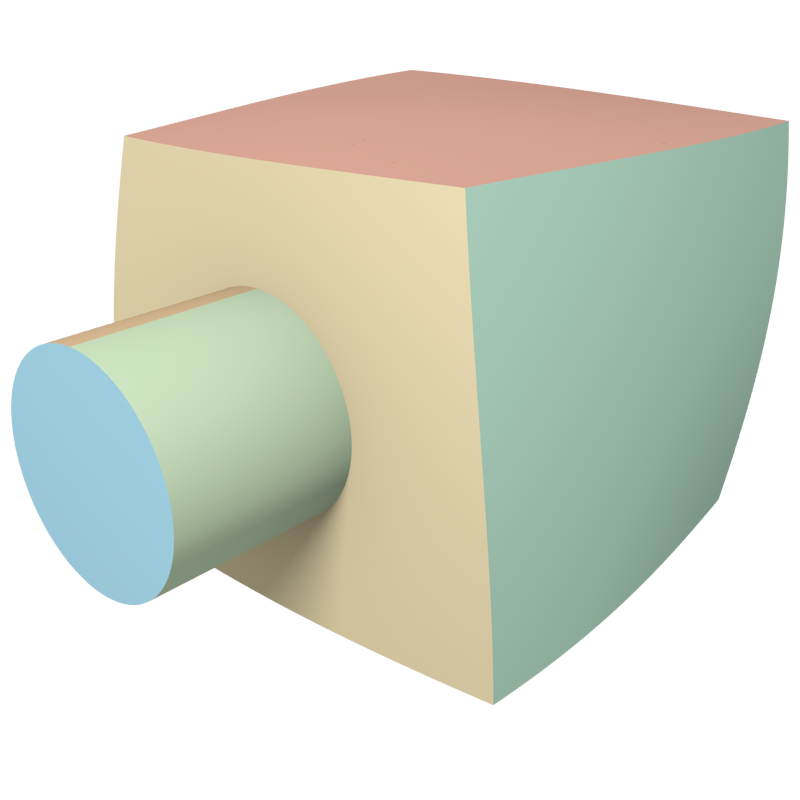
\includegraphics[width=\imw]{figures/fig_brep}};
		%%% HIDDEN EDGES
		\node[img] at (0,0) {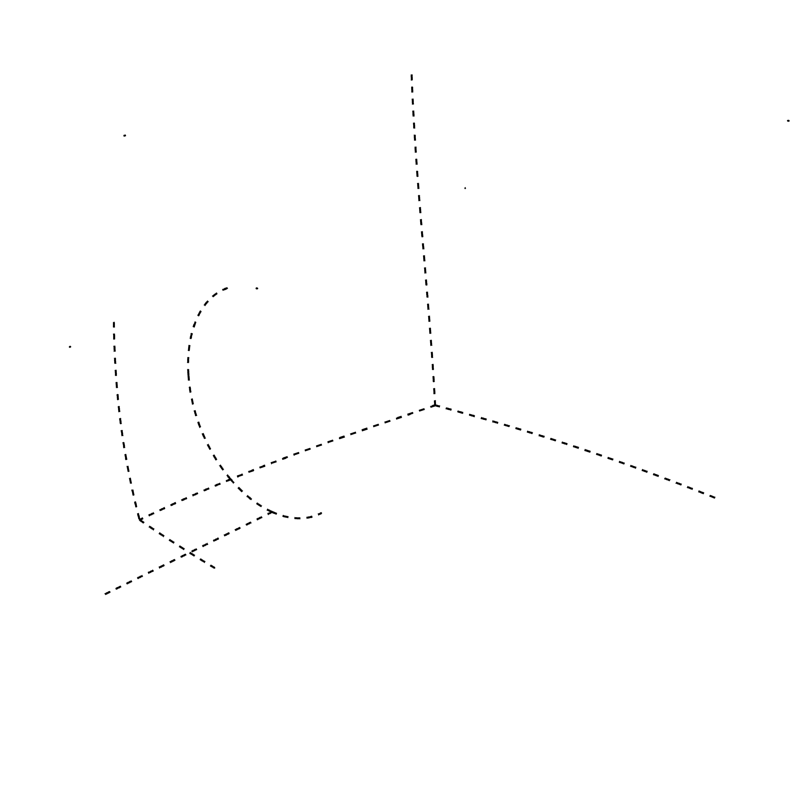
\includegraphics[width=\imw]{figures/fig_brep_edges_hid}};%
		%%% HIDDEN VERTICES
		\DTLforeach*{dbverts}{\locx=x, \locy=y, \loca=a}{%
			\ifnum \loca = 0
				\fill[black] (\locx,\locy) circle (1.0pt);
			\fi
		}%
		%%% FACES (semi-transparent to mask hidden edges & verts)
		{\transparent{0.75}
			\node[img] at (0,0) {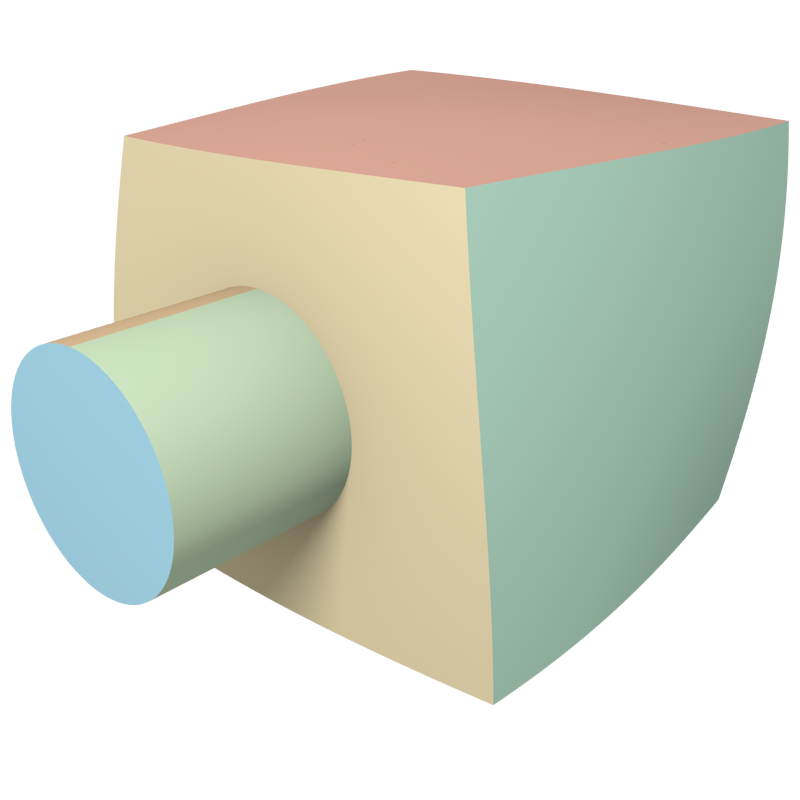
\includegraphics[width=\imw]{figures/fig_brep}};%
		}%
		%%% VISIBLE EDGES
		\node[img] at (0,0) {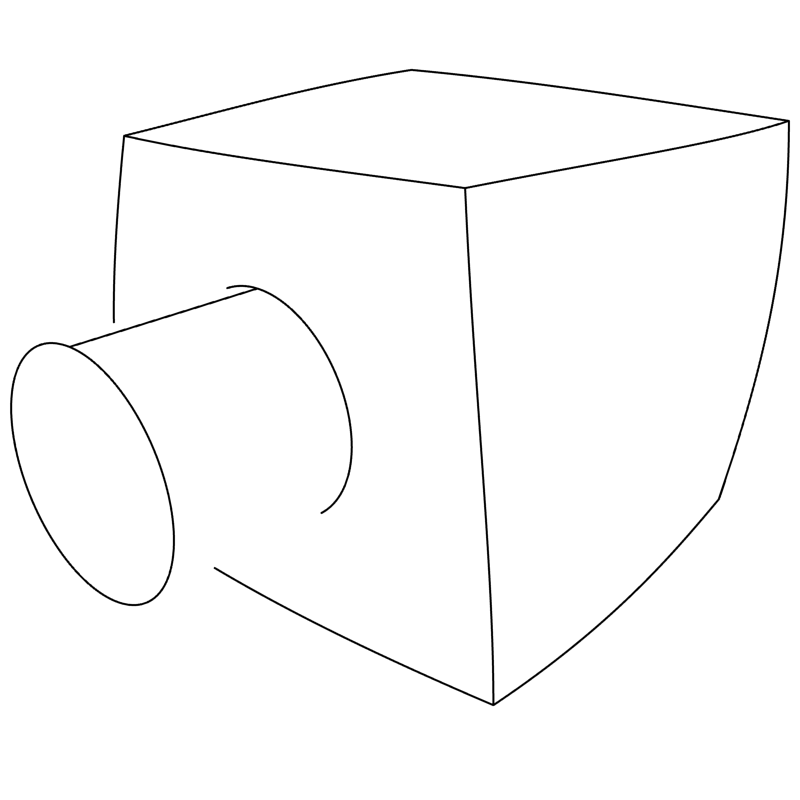
\includegraphics[width=\imw]{figures/fig_brep_edges_vis}};%
		%%% VISIBLE VERTICES
		\DTLforeach*{dbverts}{\locx=x, \locy=y, \loca=a}{%
			\ifnum \loca = 1
				\fill[black] (\locx,\locy) circle (1.0pt);
			\fi
		}%
	\end{tikzpicture}
	\DTLgdeletedb{dbverts}%
	%\hrule\par
	% DECOMPOSITION
	\def\imfacew{44mm}
	\def\ngriduv{6}
	\def\vertsep{0.05}
	\def\edglabsepuv{0.17}
	\def\wirlabsepuv{0.18}
	\def\edglabsepxyz{0.06}
	\def\iniwclr{0.3}
	\def\decwclr{0.3}%{0.2}
	\def\uvscale{0.34}
	\def\uvyshift{-0.7}
	\pgfmathsetmacro\sepyshift{0.5 * (\uvyshift+\uvscale)}%
	%
	\begin{tikzpicture}[%
		x = \imfacew, y = \imfacew,
		gridtick/.style={red, fill=white, font=\tiny, inner sep=0.5pt},
		img/.style={anchor=south west, inner sep=0},
		label/.style={inner sep=1pt, font=\scriptsize},
		uvgrid/.style={black!10!white},
		curv/.style={line width=0.8pt, line cap=round},
		spacelabel/.style={anchor=north, rotate=90, inner sep=0, font=\bfseries},
		]
		\foreach \jfa/\ifa in {-1/007, 0/008, 1/002}{%
			\figbrepface{\ifa}{{1.05*\jfa - 0.5}}{{-\sepyshift}}%\hfill
		}%
		\draw[very thick, gray, dashed] 
		({-0.5*\textwidth},0) -- ++ 
		(\textwidth,0);
		\node[spacelabel] (xyzspace) at 
		({-0.5*\textwidth},{-\sepyshift+0.5}) {Espace euclidien\vphantom{Espace paramétrique}};
		\node[spacelabel] (uvspace) at 
		({-0.5*\textwidth},{\sepyshift-\uvscale}) {Espace paramétrique\vphantom{Espace euclidien}};
%		\draw[red] (uvspace.north west) -- (xyzspace.north east);
	\end{tikzpicture}
	%\par\hrule
\end{figure}



\def\parampatchimagewidth{80mm}
\def\parampatchimageheight{60mm}
\def\uvsize{32mm}
\def\scaledpsi{0.8}
\def\fracaxeoffset{0.0}
\def\distanceaxe{0.1}
\def\scaletriedre{0.8}
\def\parampatchshadowtransparency{0.4}
\colorlet{uvbgcolor}{white!92!black}
\definecolor{ducolor}{RGB}{255,85,66}
\definecolor{dvcolor}{RGB}{40,139,226}
\definecolor{dscolor}{RGB}{46,194,75}
%
\DTLsetseparator{,}%
\DTLloaddb[noheader,keys={x,y}]{dbpointonsurf}{figures/data/fig_diffgeom_point_on_surface.dat}%
%
\DTLloaddb[noheader,keys={x,y}]{dbpointoncurv}{figures/data/fig_diffgeom_point_on_curve.dat}%
%
\begin{figure}
%\hrule\par
\centering
\begin{tikzpicture}[
	x = \parampatchimagewidth, y = \parampatchimagewidth,
	axe/.style={-stealth, line width=0.5pt},
	img/.style={anchor=south west, inner sep=0},
	axe/.style={-stealth, line width=0.5pt},
	label/.style={font=\small, inner sep=1.5pt},
	vector/.style={-latex', very thick},
	curv/.style={thick, line cap=round},
	map/.style={-{Classical TikZ Rightarrow[length=4pt,width=4pt]}}]
	%
	% XYZ-space
	\begin{scope}[shift={(0.3,0)}, 
		x = \parampatchimagewidth, y = \parampatchimageheight]
		%
		{\transparent{\parampatchshadowtransparency}%
			\node[img] at (0,0) {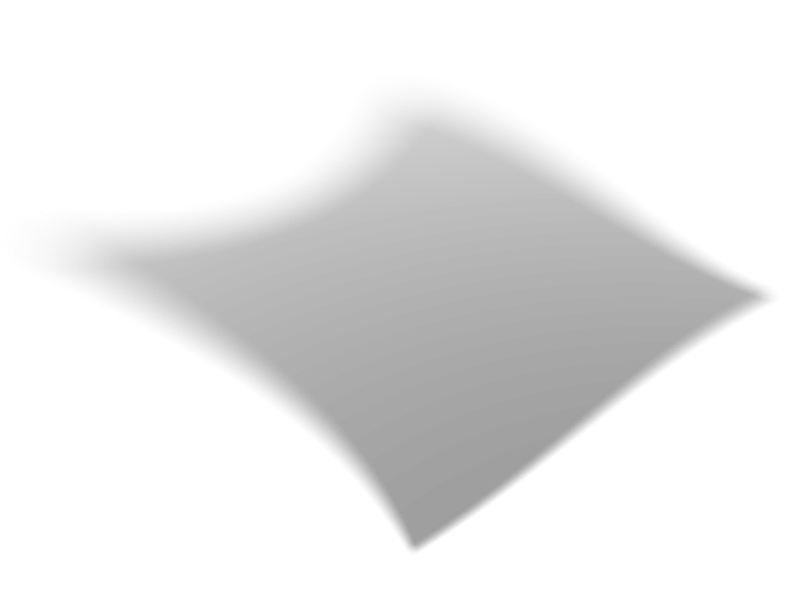
\includegraphics[width=\parampatchimagewidth]{figures/parametric_patch_shadow}};
		}%
		\node[img] at (0,0) {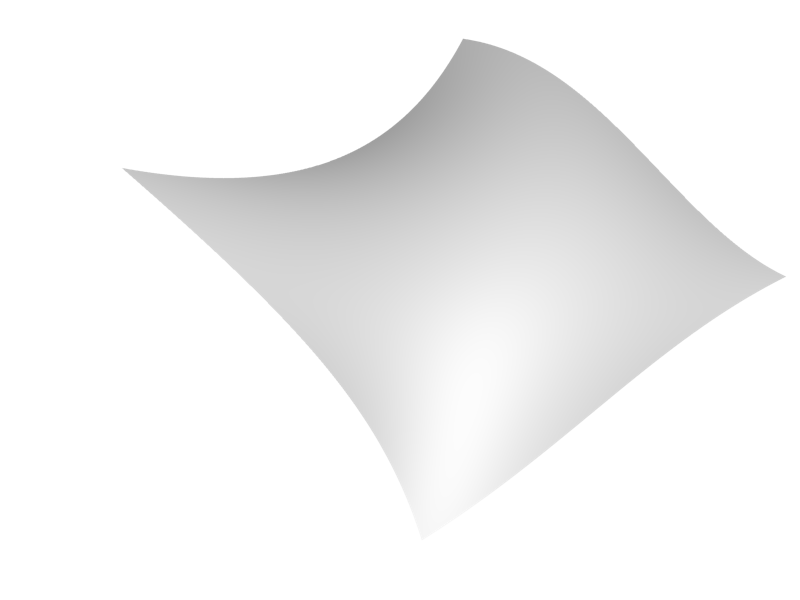
\includegraphics[width=\parampatchimagewidth]{figures/parametric_patch_surface}};
		{\transparent{0.05}%
			\node[img] at (0,0) 	{
\includegraphics[width=\parampatchimagewidth]{figures/parametric_patch_checkerboard6}};
		}%
		\node[img] at (0,0) {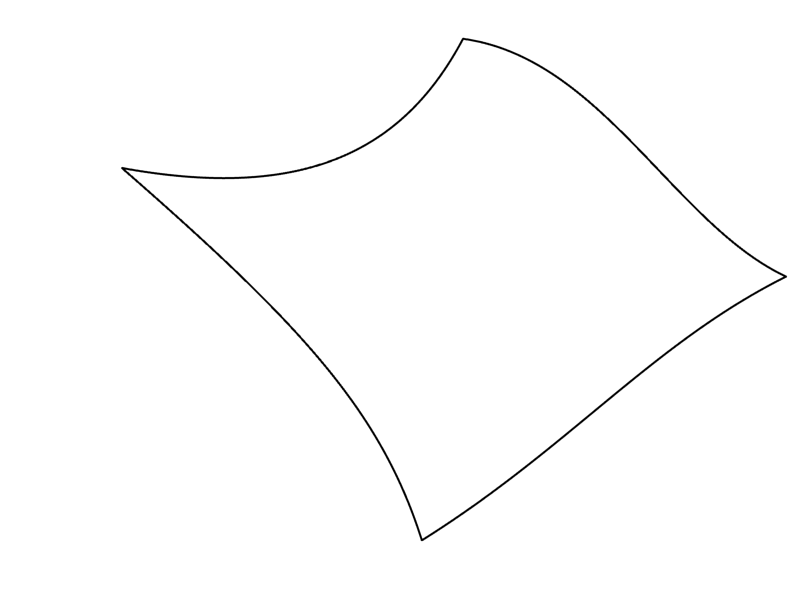
\includegraphics[width=\parampatchimagewidth]{figures/parametric_patch_border}};
		% vecteurs
		\def\scalevectors{1}
		\DTLassign{dbpointonsurf}{2}{\sxco=x,\syco=y}% 
		\DTLassign{dbpointonsurf}{4}{\suxco=x,\suyco=y}% 
		\DTLassign{dbpointonsurf}{5}{\svxco=x,\svyco=y}% 
		\DTLassign{dbpointonsurf}{6}{\nxco=x,\nyco=y}% 
		\DTLassign{dbpointonsurf}{7}{\dsxco=x,\dsyco=y}% 
		\coordinate (s) at (\sxco,\syco);
		\coordinate (su) at (\suxco,\suyco);
		\coordinate (sv) at (\svxco,\svyco);
		\coordinate (n) at (\nxco,\nyco);
		\coordinate (ds) at (\dsxco,\dsyco);
		\draw[dash pattern = on 2pt off 2pt] 
			(su) -- (ds)
			(sv) -- (ds);
		\draw[vector, ducolor] (s) -- (su);% node[label, anchor=north west] {$\bsu$};
		\draw[vector, dvcolor] (s) -- (sv);% node[label, anchor=south] {$\bsv$};
		\draw[vector, black] (s) -- (n) node[label, anchor=south] {$\unv$};
		\draw[vector, dscolor] (s) -- (ds) node[label, anchor=west] {$\dx{\bs}$};
		\fill[black] (s) circle (1.5pt);
		\node [label, anchor=east] at (s) {$\bs(\bu)$};
		%
		\draw[curv] plot file {figures/data/fig_diffgeom_xyzcurve.dat}
			node[label, anchor=east] {$\Gamma$};
		\DTLassign{dbpointoncurv}{4}{\gxco=x,\gyco=y}% 
		\DTLassign{dbpointoncurv}{5}{\dgxco=x,\dgyco=y}% 
		\coordinate (g) at (\gxco,\gyco);
		\coordinate (dg) at (\dgxco,\dgyco);
		\draw[vector] (g) -- ($(g)!\scaledpsi!(dg)$) node[label, anchor=south west] {$\bgw$};
		\fill[black] (g) circle (1.5pt);
		\node [label, anchor=south west, inner sep=0] at (g) {$\bg(w)$};
		%
		% trièdre
		\coordinate (o) at (0.7950445413589478 , 0.19190990924835205);
		\coordinate (x) at (0.6856110692024231 , 0.06267590075731277);
		\coordinate (y) at (0.9558377265930176 , 0.05519538000226021);
		\coordinate (z) at (0.822303831577301 , 0.36832109093666077);
		\draw[axe] (o) -- ($(o)!\scaletriedre!(x)$) node[label, anchor=east] {$x$};
		\draw[axe] (o) -- ($(o)!\scaletriedre!(y)$) node[label, anchor=west] {$y$};
		\draw[axe] (o) -- ($(o)!\scaletriedre!(z)$) node[label, anchor=south] {$z$};
	\end{scope}
	%
	%
	% UV-space
	\def\nuvcells{6}
	\pgfmathsetmacro\uvcellsize{2.0/\nuvcells}
	\begin{scope}[shift={(0,0.375)}, x={0.5*\uvsize}, y={0.5*\uvsize}]
		% UV-domain
		\fill[uvbgcolor] (-1,-1) -- (1,-1) -- (1,1) -- (-1,1) -- cycle;
		\foreach \locj in {1,2,...,\nuvcells}{%
			\pgfmathsetmacro\locy{-1.+(\locj-1)*\uvcellsize}
			\foreach \loci in {1,2,...,\nuvcells}{%
				\pgfmathsetmacro\locx{-1.+(\loci-1)*\uvcellsize}
				\pgfmathsetmacro\modij{int(mod(\loci + \locj,2))}
				\ifnum \modij = 0
					\fill[black!5!uvbgcolor] 
						(\locx,\locy) rectangle ++ (\uvcellsize,\uvcellsize);
				\fi
			}%
		}%
		\draw[semithick] (-1,-1) -- (1,-1) -- (1,1) -- (-1,1) -- cycle;
		% Axes
		\coordinate (o) at ({-1-\distanceaxe},{-1-\distanceaxe});
		\draw[axe] (o) -- ++ ({\fracaxeoffset+\distanceaxe+0.5},0) node [label, anchor=north west] {$u$};
		\draw[axe] (o) -- ++ (0,{\fracaxeoffset+\distanceaxe+0.5}) node [label, anchor=south east] {$v$};
		%
		\DTLassign{dbpointonsurf}{1}{\uvxco=x,\uvyco=y}% 
		\DTLassign{dbpointonsurf}{3}{\duvxco=x,\duvyco=y}% 
		\coordinate (uv) at (\uvxco,\uvyco);
		\coordinate (du) at ([shift={(\duvxco,0)}]uv);
		\coordinate (dv) at ([shift={(0,\duvyco)}]uv);
		\coordinate (duv) at ([shift={(\duvxco,\duvyco)}]uv);
		\draw[dash pattern = on 2pt off 2pt] 
			(du) -- (duv)
			(dv) -- (duv);
		\draw[vector, ducolor] (uv) -- (du);% node[label, anchor=north west] {$\dx{u}$};
		\draw[vector, dvcolor] (uv) -- (dv);% node[label, anchor=south] {$\dx{v}$};
		\draw[vector, dscolor] (uv) -- (duv) node[label, anchor=west] {$\dx{\bu}$};
		\fill[black] (uv) circle (1.5pt);
		\node [label, anchor=north, inner sep=4pt] at (uv) {$\bu$};
		%
		\draw[curv] plot file {figures/data/fig_diffgeom_uvcurve.dat}
			node[label, anchor=west] {$\Psi$};
		\DTLassign{dbpointoncurv}{2}{\uvxco=x,\uvyco=y}% 
		\DTLassign{dbpointoncurv}{3}{\duvxco=x,\duvyco=y}% 
		\coordinate (psi) at (\uvxco,\uvyco);
		\draw[vector] (psi) -- ++ 
		({\scaledpsi*\duvxco,\scaledpsi*\duvyco}) 
		node[label, anchor=south, shift={(2pt,4.5pt)}] {$\bpw$};
		\fill[black] (psi) circle (1.5pt);
		\node [label, anchor=north west, inner sep=0] at (psi) {$\bp(w)$};
		%
	\end{scope}
	%
%	\draw [dotted] (current bounding box.south west) rectangle 
%		(current bounding box.north east);
	%
	% Mappings
	\draw [draw=none] (uv) 
		to [bend left=30] 
		coordinate[pos=0.2] (c)
		coordinate[pos=0.7] (d)
		(s);
	\draw [map] (c) 
		to [bend left=20] 
		node [label, anchor=south west] {$\bs$} 
		(d);
\end{tikzpicture}
%\par\hrule
\caption{Carreau de surface paramétrique\ldots}
\end{figure}
\DTLgdeletedb{dbpointonsurf}%
\DTLgdeletedb{dbpointoncurv}%


\par\bigskip
\textit{On se place dans le cas où l'interface est une variété sans bord.}\par
Chaque arête \brep\ est alors incidente à exactement deux faces. 
Géométriquement, l'arête $\brepedge$ est représentée par une branche de la courbe d'intersection entre les carreaux de surfaces $\Sigma_1$ et $\Sigma_2$ qui décrivent respectivement les faces incidentes $\brepface_1$ et $\brepface_2$. 
Cette courbe peut également être représentée par sa trace dans l'espace paramétrique de chaque carreau de surface. 
On peut donc la représenter à l'aide des trois courbes paramétriques $\bg$, $\bp_1$ et $\bp_2$ telles que
\begin{equation}
	\bg(w) = \bs_1(\bp_1(w)) = \bs_2(\bp_2(w)),
\end{equation}
pour tout $w$.\\
En pratique, seule une approximation de la véritable courbe d'intersection peut être obtenue, si bien que ces trois représentations ne coïncident pas exactement.
Plusieurs approches sont envisageables :
\begin{itemize}
	\item paramétrisation approchée (\eg spline)
	\begin{itemize}
		\item avantages : représentation continue, évaluation directe
		\item inconvénient : ne correspond à la véritable intersection qu'en certains points
	\end{itemize}
	\item courbe procédurale
	\begin{itemize}
		\item approximation linéaire par morceaux dont chaque n\oe ud est situé \guill{exactement} sur l'intersection
		\item l'espacement des n\oe ud est dicté par un critère pour contrôler l'\textit{erreur de corde}
		\item les points intermédiaires sont évalués par raffinement itératif (procédure à détailler)
		\item avantage : contrôle précis de la précision
		\item inconvénient : évaluation plus coûteuse 
	\end{itemize}
\end{itemize}

%\begin{figure}
%\centering
%\includegraphics[width=12cm]{figures/brep_edge_dual_geometric_representation}
%\caption{Description géométrique d'une arête \brep.}
%\end{figure}


\begin{figure}
%\hrule\par
\centering
\newlength{\locimw}
\setlength{\locimw}{67.5mm}
\newlength{\locimh}
\setlength{\locimh}{\locimw * \real{0.75}}
%
\def\uvscale{0.28}
\def\fracaxeoffset{0.0}
\def\distanceaxe{0.1}
\def\psisep{-0.42}
%
\DTLsetseparator{,}%
\DTLloaddb[noheader,keys={x,y}]{dbpoint}{figures/data/fig_simple_intersection_point.dat}%
\DTLassign{dbpoint}{1}{\xloc=x, \yloc=y}% 
%
\begin{tikzpicture}[
	x=\locimw, y=\locimh, 
	axe/.style={-stealth, line width=0.5pt},
	uvdomain/.style={thin}, 
	image/.style={anchor=south west, inner sep=0},
	curve/.style={thick, line cap=round},
	label/.style={font=\normalsize},
	axelabel/.style={font=\small},
	axeuvlabel/.style={axelabel, inner sep=0},
	point/.style={fill=black, circle, scale=0.3},
	map/.style={-{Classical TikZ Rightarrow[length=4pt,width=4pt]}}]
	%
	\node[image] (img) at (0,0) {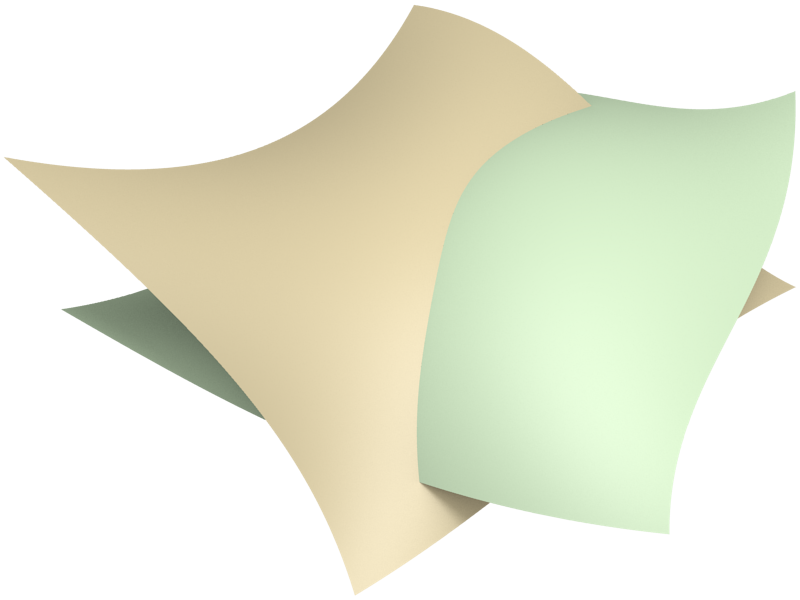
\includegraphics[width=\locimw]{figures/fig_simple_intersection}};
	\node[image] (img) at (0,0) {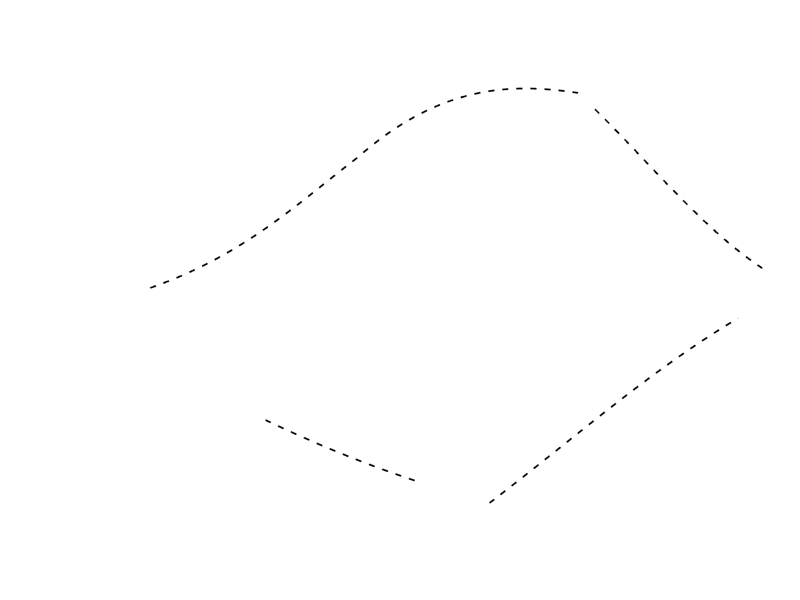
\includegraphics[width=\locimw]{figures/fig_simple_intersection_border_hid}};
	{\transparent{0.75}%
		\node[image] (img) at (0,0) {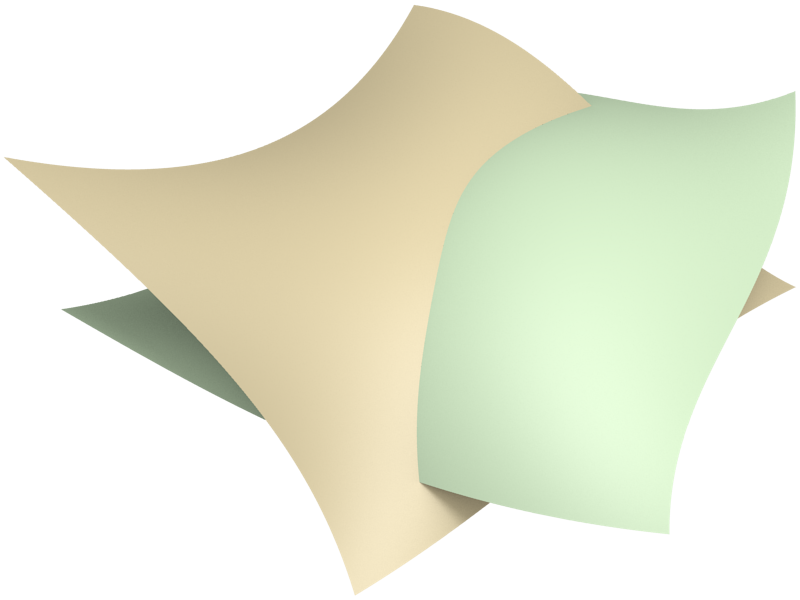
\includegraphics[width=\locimw]{figures/fig_simple_intersection}};
	}%
	\node[image] (img) at (0,0) {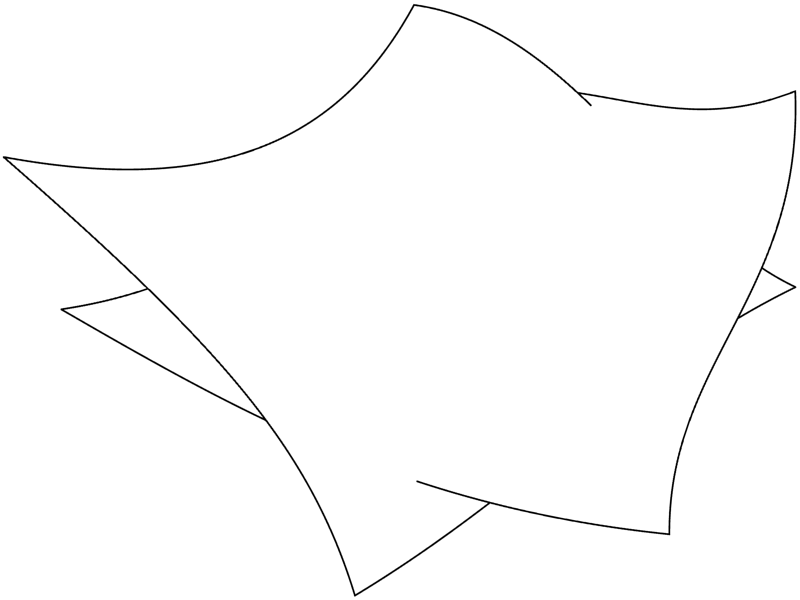
\includegraphics[width=\locimw]{figures/fig_simple_intersection_border_vis}};
	\draw[curve] plot file {figures/data/fig_simple_intersection_curve.dat};
	\node[point] (xyz) at (\xloc, \yloc) {};
	\node[label, anchor=east] at (\xloc, \yloc) {$\bg(w)$};
	%
	\node[label] at (0.56, 0.91) {$\Sigma_1$};
	\node[label] at (0.93, 0.75) {$\Sigma_2$};
	%
%	\foreach \igrid in  {0,0.1,...,1.01}{
%		\draw[red, thin] (0,\igrid) -- (1,\igrid)
%		                 (\igrid,0) -- (\igrid,1);
%	}
	% 
	% trièdre
	\def\scaletriedre{0.8}
	\coordinate (o) at (0.13209545612335205 , 0.14773482084274292);
	\coordinate (x) at (0.23464959859848022 , 0.02938912808895111);
	\coordinate (y) at (0.26169726252555847 , 0.2535654902458191);
	\coordinate (z) at (0.1061694324016571 , 0.31903284788131714);
	\draw[axe] (o) -- ($(o)!\scaletriedre!(x)$) node[axelabel, anchor=west] {$x$};
	\draw[axe] (o) -- ($(o)!\scaletriedre!(y)$) node[axelabel, anchor=west] {$y$};
	\draw[axe] (o) -- ($(o)!\scaletriedre!(z)$) node[axelabel, anchor=south] {$z$};
	%
	\begin{scope}[scale=\uvscale, x=\locimh, y=\locimh, shift={(img.west)}]
		\begin{scope}[shift={(-1.5,0.7)}]
			\DTLloaddb[noheader,keys={r,g,b}]{dbsurfacecolor}{figures/data/fig_brep_faces/facecolor_002.dat}%
			\DTLassign{dbsurfacecolor}{1}{\rfai=r,\gfai=g,\bfai=b}% 
			\definecolor{surfacecolor}{RGB}{\rfai,\gfai,\bfai}
			\draw[uvdomain, fill=surfacecolor] (-1,-1) -- (1,-1) -- (1,1) -- (-1,1) -- cycle;
			\DTLgdeletedb{dbsurfacecolor}
			%
			\draw[curve] plot file {/d/bandrieu/GitHub/FFTsurf/test/demo_intersection/simple/curve_uv1.dat};
			%
			\DTLassign{dbpoint}{2}{\uloc=x, \vloc=y}% 
			\DTLassign{dbpoint}{3}{\duloc=x, \dvloc=y}% 
			\node[point] (uv1) at (\uloc, \vloc) {};
			%\node[label] at ({\uloc + \psisep*\duloc}, {\vloc + \psisep*\dvloc}) {$\bp_1(w)$};
			\node[label, anchor=north east, inner sep=0] at (\uloc, \vloc) {$\bp_1(w)$};
			% Axes
			\coordinate (o) at ({-1-\distanceaxe},{-1-\distanceaxe});
			\draw[axe] (o) -- ++ ({\fracaxeoffset+\distanceaxe+0.5},0) node [axeuvlabel, anchor=north west] {$u_1$};
			\draw[axe] (o) -- ++ (0,{\fracaxeoffset+\distanceaxe+0.5}) node [axeuvlabel, anchor=south east] {$v_1$};
		\end{scope}
	\end{scope}
	%
	\begin{scope}[scale=\uvscale, x=\locimh, y=\locimh, shift={(img.east)}]
		\begin{scope}[shift={(1.6,-0.9)}]
			\DTLloaddb[noheader,keys={r,g,b}]{dbsurfacecolor}{figures/data/fig_brep_faces/facecolor_008.dat}%
			\DTLassign{dbsurfacecolor}{1}{\rfai=r,\gfai=g,\bfai=b}% 
			\definecolor{surfacecolor}{RGB}{\rfai,\gfai,\bfai}
			\draw[uvdomain, fill=surfacecolor] (-1,-1) -- (1,-1) -- (1,1) -- (-1,1) -- cycle;
			\DTLgdeletedb{dbsurfacecolor}
			%
			\draw[curve] plot file {/d/bandrieu/GitHub/FFTsurf/test/demo_intersection/simple/curve_uv2.dat};
			%
			\DTLassign{dbpoint}{4}{\uloc=x, \vloc=y}% 
			\DTLassign{dbpoint}{5}{\duloc=x, \dvloc=y}% 
			\node[point] (uv2) at (\uloc, \vloc) {};
			%\node[label] at ({\uloc + \psisep*\duloc}, {\vloc + \psisep*\dvloc}) {$\bp_2(w)$};
			\node[label, anchor=north east, inner sep=0] at (\uloc, \vloc) {$\bp_2(w)$};
			% Axes
			\coordinate (o) at ({-1-\distanceaxe},{-1-\distanceaxe});
			\draw[axe] (o) -- ++ ({\fracaxeoffset+\distanceaxe+0.5},0) node [axeuvlabel, anchor=north west] {$u_2$};
			\draw[axe] (o) -- ++ (0,{\fracaxeoffset+\distanceaxe+0.5}) node [axeuvlabel, anchor=south east] {$v_2$};
		\end{scope}
	\end{scope}
	%
	% mappings
	\draw [map, shorten <= 5mm, shorten >= 5mm] (uv1) to [bend left =40] node [label, anchor=south west] {$\bs_1$} (xyz);
	\draw [map, shorten <= 5mm, shorten >= 5mm] (uv2) to [bend right=40] node [label, anchor=south west] {$\bs_2$} (xyz);
	%
%	\draw[red, thin, dashed] (current bounding box.south west) rectangle (current bounding box.north east);
\end{tikzpicture}
\DTLgdeletedb{dbpoint}
%\par\hrule
\caption{Description géométrique d'une arête \brep.}
\end{figure}


\section{Contributions}% aka "Description de la thèse/démarche"


\section{Organisation du manuscrit}

\chapter[Algorithme de propagation d'interfaces régulières par morceaux]{Algorithme général pour la propagation d'interfaces régulières par morceaux}

\textit{on veut mettre en place un algorithme basé sur le principe de Huygens (avec condition d'entropie) pour simuler la propagation d'une interface représentée suivant le formalisme \brep, i.e. pour construire un nouveau modèle \brep~(géométrie et topologie) correspondant à une enveloppe de boules (EdB) centrées sur l'interface courante.}


\section{Traitement des différentes entités \brep}
on construit d'abord une EdS (partielle), puis on la transforme en EdB pour respecter la condition d'entropie. Chaque entité du modèle \brep~est traitée spécifiquement

vitesse normale continue $\Rightarrow$ rayon des sphères évolue continument 
sur toute l'interface
\subsection{Traitement des faces}
chaque face repose sur une surface orientée de continuité géométrique élevée (d'ordre 1 ou plus) donc chaque point sur une face a exactement 2 vis-à-vis sur l'EdS (un dans le sens de la normale, et un dans le sens opposé) (sous réserve d'une condition, détaillée dans la \Sref{sec:EdS_2param})


\subsection{Traitement des arêtes}
\begin{itemize}
	\item douce $\to$ préservée car vitesse continue ;
	\item (vive) convexe $\to$ EdS à un paramètre (nouvelle(s) \textit{sur}face(s)) ;
	\item (vive) concave $\to$ aucune influence sur l'EdB (on ne construit pas son EdS, d'où le ``partiel'') ;
\end{itemize}

\subsection{Traitement des sommets}
\begin{itemize}
	\item smooth $\to$ préservé car vitesse continue ;
	\item convexe $\to$ nouvelle(s) \textit{sur}face(s) sphérique(s) ;
	\item concave $\to$ aucune influence sur l'EdB.
\end{itemize}


%\begin{itemize}
%	\item faces $\to$ EdS à deux paramètres (justifier) ;
%	\item arêtes
%	\begin{itemize}
%		\item douce $\to$ préservée car vitesse continue ;
%		\item (vive) convexe $\to$ EdS à un paramètre (nouvelle(s) \textit{sur}face(s)) ;
%		\item (vive) concave $\to$ aucune influence sur l'EdB (on ne construit pas son EdS, d'où le ``partiel'') ;
%	\end{itemize}
%	\item sommets
%	\begin{itemize}
%		\item smooth $\to$ préservé car vitesse continue ;
%		\item convexe $\to$ nouvelle(s) \textit{sur}face(s) sphérique(s) ;
%		\item concave $\to$ aucune influence sur l'EdB.
%	\end{itemize}
%\end{itemize}

%\section{Ce titre de section est vraiment trop long,\newline il faudrait trouver un moyen de le raccourcir,\newline il s'étend sur plusieurs lignes, c'est beaucoup trop long}


\section{Construction de l'enveloppe des sphères}%{Construction géométrique de l'enveloppe des sphères}

\subsection{Enveloppe d'une famille de sphères à un paramètre}
%\subsection{Enveloppe d'un ensemble de sphères à un paramètre}
\eng{canal surfaces} \cite{peternell1997} (\eng{spine curve} $\to$ squelette (ou axe médian))

\subsection{Enveloppe d'une famille de sphères à deux paramètres}
\label{sec:EdS_2param}
extension \eng{canal surfaces} \cite{gelston1995}\\
différence avec le simple transport suivant la normale \cite{jiao2001}




\section{Application de la condition d'entropie}
résolution des intersections (pas encore de détail sur la méthode) $\to$ faces trimmées, nouveaux sommets/arêtes

\subsection{Reconstitution topologique du modèle \brep}
Intersections de paires de surfaces ($\to$ courbes\footnote{dans le cas général, non-dégénéré (cf. cours ``Topologie et géométrie différentielle'')\label{foot}}), de triplets de surface (ou de paires de courbes) ($\to$ points\textsuperscript{~\ref{foot}})\\
graphe d'adjacence des surfaces, courbes, points \cite[Chap. 4]{pentcheva2010}\\
formation des faces (\eng{wires} $\to$ chaînes?) \cite[Chap. 7]{pentcheva2010}, arêtes et sommets \cite[Chap. 5]{pentcheva2010}

\ldots



\bigskip
\textit{il faut maintenant faire le choix d'une méthode numérique pour appliquer cet algorithme de façon pratique\ldots}

\chapter{Méthode d'ordre élevé pour le suivi d'un carreau de surface}%patch surfacique rectangulaire}
\label{chap:methode_ps}

\textit{on veut mettre au point une méthode numérique (discrétisations spatiale et temporelle) pour le suivi d'un seul patch rectangulaire de surface de continuité géométrique élevée (infinie), qui servira de base pour  mettre en \oe uvre l'algorithme du \autoref{chap:algo_general}}
\par\bigskip

suivi lagrangien de marqueurs/points de collocation situés sur la surface

\section{Discrétisation spectrale en espace}%spatiale}
méthode pseudo-spectrale : solution développée dans une base de fonctions globales et régulières, résidu annulé exactement en un nombre discret de points de collocation, donnant une EDO en temps par point de collocation\par
Choix des fonctions de base et des marqueurs/points de collocation\par

\subsection{État de l'art}
Le choix des fonction de base se pose alors. Celles-ci doivent pouvoir représenter n'importe quel type de solution avec une précision arbitraire, offrir une convergence rapide à mesure que le nombre de degrés de liberté augmente et enfin pouvoir être évaluées efficacement. A ces critères s'ajoutent également des contraintes liées à la topologie de la solution (i.e. l'interface en propagation).\par

Traditionnellement, les méthodes spectrales reposent sur les séries de Fourier lorsque la solution est spatialement périodique. 
Les polynômes trigonométriques ont ainsi été utilisés comme fonctions de base pour représenter un front de flamme dans une configuration quasi-3{\scshape d} \cite{gueyffier2015} (\textbf{reformuler}).
Lorsque la solution est une surface fermée de genre zéro (\ie une sphère topologique), la base des harmoniques sphériques est particulièrement adaptée \cite{veerapaneni2011}.\par
Les travaux de Bruno \cite{bruno2007} sur une méthode de \eng{continuation} ont permis d'étendre l'usage des polynômes trigonométriques aux surfaces homéomorphes à des disques. 
Cette approche permet de représenter des surfaces de géométrie complexe et de topologie arbitraire en raccordant des patchs locaux à l'aide de partitions de l'unité.\\
\textbf{Permet d'éviter Gibbs dans le cas régulier par morceaux}\\
A l'instar de la méthode proposée dans cette thèse, l'idée est alors de représenter des surfaces de géométrie complexe et de topologie arbitraire à l'aide de paramétrisations locales en construisant un atlas. 
En revanche, cette approche nécessite la résolution de systèmes linéaires mettant en jeu des matrices de grande taille, pleines et généralement mal conditionnées. 
En outre, cette méthode n'a à ce jour pas été appliquée pour la déformation de surface.
%Ce type de discrétisation spectrale a notamment été utilisé pour la représentation de vésicules inextensibles en suspension dans un écoulement fortement visqueux \cite{veerapaneni2011}. 
%Dans ces travaux, la base des harmoniques sphériques est naturellement adaptée à la topologie des vésicules (genre 0 sans bord).
%Les polynômes trigonométriques ont également été utilisés comme fonctions de base pour représenter un front de flamme une configuration quasi-3{\scshape d} \cite{gueyffier2015}.

\begin{itemize}
	\item harmoniques sphériques \cite{veerapaneni2011}, polynômes trigonométriques \cite{gueyffier2015} $\to$ contraintes topologiques (genre 0, sans bord ou périodique) (méthode de continuation \cite{bruno2007} pour s'affranchir de cette contrainte, mais complexe (POUs, \ldots) et jamais utilisé pour des surfaces en mouvement)
	\item CAO : courbes/surfaces polynomiales (algébriques)/rationnelles (en produit tensoriel) par morceaux (B-splines/NURBS), utilisant la base de Bernstein
	\begin{equation}
		B_n^N(x) = \binom{N}{n} \left( 1 - x \right)^{N-n} x^n.
	\end{equation}
	\begin{itemize}
		\item[+] coefficients = points de contrôle dans l'espace physique, sens géométrique intuitif
		\item[+] partition de l'unité sur $\berninterval$ $\Rightarrow$ propriété d'enveloppe convexe
		\item[-] algorithme d'évaluation (de Casteljau) numériquement stable mais coûteux $\bigO{N^2}$
		\item[-] points de contrôle pas \emph{sur} la courbe/surface $\Rightarrow$ pas exploitables comme marqueurs lagrangiens
		\item[-] peu pratiques pour réduire/élever le degré des polynômes
	\end{itemize}
\end{itemize}
\bigskip
on choisit les polynômes de Chebyshev, couramment employés dans les méthodes spectrales dans le cas non-périodique
%on choisit les polynômes de Chebyshev\footnotemark, couramment employés dans les méthodes spectrales dans le cas non-périodique
%\footnotetext{En français, le nom de ce mathématicien russe est généralement orthographié \guill{Tchebychev}. Nous utiliserons cependant l'orthographe anglo-saxone, plus couramment utilisée par la communauté scientifique.}
%(Mason, p.81) >>>-----
%Orthogonal polynomials have a great variety and wealth of properties,
%many of which are noted in this chapter. Indeed, some of these properties
%take a very concise form in the case of the Chebyshev polynomials, making
%Chebyshev polynomials of leading importance among orthogonal polynomi-
%als — second perhaps to Legendre polynomials (which have a unit weight
%function), but having the advantage over the Legendre polynomials that the
%locations of their zeros are known analytically. Moreover, along with the Legendre polynomials, the Chebyshev polynomials belong to an exclusive band
%of orthogonal polynomials, known as Jacobi polynomials, which correspond
%to weight functions of the form (1 − x) α (1 + x) β and which are solutions of
%Sturm–Liouville equations.
%The Chebyshev polynomials have further properties, which are peculiar
%to them and have a trigonometric origin, namely various kinds of discrete
%orthogonality over the zeros of Chebyshev polynomials of higher degree. In
%consequence, interpolation at Chebyshev zeros can be achieved exceptionally
%inexpensively (Chapter 6) and Gauss quadrature methods based on Cheby-
%shev zeros are extremely convenient (Chapter 8).
%<<<-----



\subsection{Polynômes de Chebyshev}
Les polynômes de Chebyshev sont très largement utilisés dans de nombreux domaines tels que l'analyse numérique.
L'objet des sections suivantes est de rappeler la définition de cette famille 
de polynômes et d'en présenter brièvement les propriétés remarquables qui seront exploitées dans cette thèse. 
Nombreux sont les ouvrages consacrés aux polynômes de Chebyshev \cite{mason2002, gil2007} ainsi qu'à leur usage dans les méthodes spectrales \cite{boyd2001, canuto2006}, aussi le lecteur est invité à s'y référer pour plus de détails.


\subsubsection{Définition et propriétés}
\begin{definition}
	Pour $n \in \mathbb{N}$, le polynôme de Chebyshev (de première espèce) $T_n$ est défini par%un polynome de degré $n$ défini par
	\begin{equation}
		T_n(\cos \theta) = n \cos \theta.
		\label{eq:chebyshev_trigo}
	\end{equation}
\end{definition}
%De la définition \eqref{eq:chebyshev_trigo} et de l'identité trigonométrique
De cette définition et de l'identité trigonométrique $\cos n\theta + \cos (n-2)\theta = 2\cos \theta \cos (n-1)\theta$, on peut déduire la relation de récurrence suivante, pour $x \in \chebinterval$, 
\begin{align}[left = \empheqlbrace\,]
	T_0(x) &= 1, \nonumber\\
	T_1(x) &= x, \nonumber\\
	T_n(x) &= 2x T_{n-1}(x) - T_{n-2}(x) \text{,\ pour\ } n \geq 2.
	\label{eq:chebyshev_recurrence}
\end{align}
Le graphe des six premiers polynômes de Chebyshev est tracé sur la \autoref{fig:chebyshev_polynomials}.\par

\begin{figure}
	\centering
	\begin{tikzpicture} 
	\begin{axis}[%
		width=8cm, height=6cm,
		axis lines*=left,
		xmin=-1.0, xmax=1.0, ymin=-1.0, ymax=1.0,
		grid=major,
		clip marker paths=false,
		enlargelimits={abs=0.05},
		xlabel={$x$},
		ylabel={$T_n(x)$},
		legend style={at={(1.025,0.5)}, anchor=west},
		no marks,
		samples=200
		]%
		\addplot+[domain=-1:1] {1.0};%
		\addplot+[domain=-1:1] {x};%
		\addplot+[domain=-1:1] {2.0*x^2 - 1.0};%
		\addplot+[domain=-1:1] {4.0*x^3 - 3.0*x};%
		\addplot+[domain=-1:1] {8.0*x^4 - 8.0*x^2 + 1.0};%
		\addplot+[domain=-1:1] {16.0*x^5 - 20.0*x^3 + 5.0*x};%
		\legend{{$T_0$},{$T_1$},{$T_2$},{$T_3$},{$T_4$},{$T_5$}}%
	\end{axis} 
\end{tikzpicture}
	\caption{Graphe des premiers polynômes de Chebyshev.}% $(n=0,\ldots,5)$ sur l'intervalle $\chebinterval$.}
	\label{fig:chebyshev_polynomials}
\end{figure}

%\begin{figure}
%	\centering
%	\begin{tikzpicture}
%		\begin{axis}[
%			width=12cm, height=9cm,
%		    set layers=standard,
%		    domain=-1:1,
%		    xmin=-1, xmax=1,
%		    zmin=-1, zmax=1,
%		    samples y=1,
%		    view={40}{30},
%		    grid = major,
%		    axis lines* = left,
%		    unit vector ratio*=4 3 1,
%		    xtick={-1,-0.5,0,0.5,1},
%		    ytick={0,1,2,3,4,5},
%		    ztick={-1,0,1},
%		    xlabel={$x$},
%		    ylabel={$n$},
%		    zlabel={$T_n(x)$},
%		    no marks,
%		    samples=201,
%		    every tick label/.append style={font=\small},
%		    %tick align=outside,
%		%    cycle list/GnBu-9,%RdYlBu-6,%Spectral-6,
%		%	cycle multiindex* list={GnBu-9},%RdYlBu-6}%Spectral-6}
%		    clip=false]
%			\pgfplotsinvokeforeach{0,1,...,5}{%
%				\addplot3+[domain=-1:1]	({x},#1,{ cos(#1*acos(x)) });
%			}%
%		\end{axis}
%	\end{tikzpicture}
%	\caption{Graphe des premiers polynômes de Chebyshev.}
%\end{figure}
%
%\begin{figure}
%	\centering
%	\begin{tikzpicture} 
%		\begin{axis}[%
%			width=8cm, height=6cm,
%			axis lines*=left,
%			xmin=-1.0, xmax=1.0, ymin=-1.0, ymax=1.0,
%			grid=major,
%			clip marker paths=false,
%			enlargelimits={abs=0.05},
%			xlabel={$x$},
%			ylabel={$T_n(x)$},
%			legend style={at={(1.025,0.5)}, anchor=west},
%			no marks,
%			samples=201,
%			%cycle list/GnBu-9,%RdYlBu-6,%Spectral-6,
%			%cycle multiindex* list={GnBu-9}%RdYlBu-6}%Spectral-6}
%			]%
%			\pgfplotsinvokeforeach{0,1,...,5}{%
%	      		\addplot+[domain=-1:1] { cos(#1*acos(x)) } coordinate[pos=0.8+#1*0.011] (x#1);
%%	      		\pgfmathparse{0.75}\let\xa\pgfmathresult
%%	      		\pgfmathparse{cos(#1*acos(0.75))}\let\ya\pgfmathresult
%%	      		\pgfmathparse{0.75-#1*0.25}\let\yb\pgfmathresult
%	      		%\def\xa{\pgfmathparse{0.75}\pgfmathresult}
%	      		%\def\ya{\pgfmathparse{cos(#1*acos(\xa))}\pgfmathresult}
%	      		%\xdef\ya{1.0 - #1*0.15}
%	      		%\xdef\xa{cos(acos(\ya)/#1)}
%	      		%\def\yb{\pgfmathparse{0.75-#1*0.25}\pgfmathresult}
%	        	%\addlegendentry{$T_{#1}$}
%	        	\draw[latex-, black, thin] 
%	        		(x#1)
%	        		to [bend right=20] 
%	        		(axis cs:1.1,1-2*#1/5) 
%	        		node [anchor=west] {$n=#1$};
%	        }%
%		\end{axis} 
%	\end{tikzpicture}
%	\caption{Graphe des premiers polynômes de Chebyshev $(n=0,\ldots,5)$ sur l'intervalle $\chebinterval$.}
%%	\label{fig:chebyshev_polynomials}
%\end{figure}

%En posant $x = \cos \theta$, il vient
%\begin{equation}
%	\dfdx{T_n(x)}{x} = \frac{n \sin n\theta}{\sin \theta}.
%\end{equation}

$T_n$ est un polynôme de degré $n$ %de coefficient dominant $2^{n-1}$ 
qui atteint ses extrema locaux sur $\chebinterval$ aux $n+1$ n\oe uds de Chebyshev-Gauss-Lobatto (CGL)%\footnote{Seuls les $n-1$ n\oe uds intérieurs sont réellement des extrema au sens où la dérivée s'y annule. A noter également que ces n\oe uds sont rangés en ordre décroissant.}
\begin{equation}
	x_k = \cos \frac{k \pi}{n},
	\label{eq:cgl_nodes}
\end{equation}
pour $0 \leq k \leq n$. 
Seuls les $n-1$ n\oe uds intérieurs sont réellement des extrema au sens où la dérivée s'y annule. 
A noter également que ces n\oe uds sont rangés en ordre décroissant.\par
Comme illustré sur la \autoref{fig:cgl_nodes}, ces extrema sont alternativement des maxima puis des minima, tous égaux en valeur absolue
\begin{equation}
	T_n(x_k) = (-1)^{k}.
	\label{eq:chebyshev_equioscillation}
\end{equation}

\begin{figure}
	\centering
	\begin{tikzpicture} 
	\begin{axis}[%
		width=8cm, height=6cm,
		axis lines*=left,
		xmin=-1.0, xmax=1.0, ymin=-1.0, ymax=1.0,
		grid=major,
		clip marker paths=false,
		enlargelimits={abs=0.05},
		]%
		\addplot+[samples=200, domain=0:pi, no marks, s6] ({cos(deg(x))}, {cos(5*deg(x))});%
		% extrema
		\addplot+[samples=6, domain=0:pi, ycomb, dashed, mark=none, black] ({cos(deg(x))}, {cos(5*deg(x))});%
		\addplot+[samples=6, domain=0:pi, only marks, mark=*, black] ({cos(deg(x))}, {0});%
		% zeros
%		\pgfplotsinvokeforeach{0,...,4}{
%			\addplot+[mark=*, red] coordinates {(cos((2.0*#1+1.0)*180.0/10.0),0)};
%		}
	\end{axis} 
\end{tikzpicture}
%	\caption{N\oe uds de Chebyshev-Gauss-Lobatto pour $n = 6$ (extrema locaux du polynome $T_6$ sur l'intervalle $\chebinterval$).}
	\caption{N\oe uds de Chebyshev-Gauss-Lobatto (extrema locaux) du polynôme $T_5$.}% sur l'intervalle $\chebinterval$.}
	\label{fig:cgl_nodes}
\end{figure}

%Cette propriété dite d'\emph{équioscillation} a pour conséquence --- via un théorème attribué au mathématicien Émile Borel --- que la meilleure approximation uniforme (\ie en norme $L_\infty$) polynomiale de degré $n - 1$ de la fonction $x \mapsto x^n$ sur $\chebinterval$ est la fonction $x \mapsto x^n - 2^{1 - n} T_n(x)$. \\
%$\to$ économisation\ldots
Cette propriété d'\emph{équioscillation} a pour conséquence le théorème suivant.
\begin{theoreme}
	Le polynôme %$p_{N-1}$ 
	de degré $N-1$ qui donne la meilleure approximation uniforme (\ie en norme $L_\infty$) %de la fonction $x \mapsto x^N$ est $p_{N-1} : x \mapsto x^N - 2^{1 - N} T_n(x)$. 
du polynôme %$q : x \mapsto \sum_{n=0}^{N} a_n x^n$
$q = \sum_{n=0}^{N} a_n X^n$ 
sur l'intervalle $\chebinterval$ est
	\begin{equation}
		p_{N-1} = q - 2^{1-N} a_N T_N,
	\end{equation}
	et, pour tout $x \in \chebinterval$,
	%La meilleure approximation %uniforme (\ie en norme $L_\infty$) 
	%polynomiale de degré $N - 1$ en norme $L_\infty$ de la fonction $x \mapsto x^N$ sur $\chebinterval$ est la fonction $p_N : x \mapsto x^N - 2^{1 - N} T_n(x)$ et
	\begin{equation}
		%\norminf{q - p_{N-1}} = 2^{1-N} \left| a_N \right|.
		\left| q(x)-  p_{N-1}(x)\right| \leq 2^{1-N} \left| a_N \right|,
	\end{equation}
	l'égalité étant atteinte aux $N+1$ n\oe uds CGL de $T_N$.
\end{theoreme}
Ce théorème trouve une application immédiate dans l'économisation des séries \textit{(à développer\ldots)}.

\subsubsection{Approximation de fonctions}
%série $\series{f}$\\
%orthogonalité $\to$ meilleure approximation polynomiale en norme $\mathcal{L}_2$ $\to$ projeté/série tronquée $\truncseries{f}{N}$, erreur de troncature\\
%polynôme d'interpolation $\interpolant{f}{N}$, orthogonalité discrète, DCT, erreur d'aliasing \par\bigskip
Notons $\Ltwospace$ l'espace de Hilbert des fonctions de carré intégrable sur $\chebinterval$, muni du produit scalaire
\begin{equation}
	\scalprod{f}{g} =
	\int_{-1}^{1} \frac{f(x) g(x)}{\sqrt{1 - x^2}} \dx{x} .
	\label{eq:chebyshev_scalar_product}
\end{equation}

La famille des polynômes de Chebyshev est une base orthogonale et maximale de cet espace, et pour tous $m,n \in \mathbb{N}$,
\begin{equation}
	\scalprod{T_m}{T_n} =
	\frac{\pi}{2} \alpha_n \delta_{m,n},
	\label{eq:chebyshev_orthogonality}
\end{equation}
où $\delta_{\cdot,\cdot}$ représente le symbole de Kronecker, et
\begin{equation}
	\alpha_n = 
	1 + \delta_{0,n}.
%	\begin{cases}
%	 2 & \text{\ si\ } n = 0,   \\ 
%	 1 & \text{\ si\ } n > 0.\\ 
%	\end{cases}
\end{equation}

%Le développement en série de Chebyshev d'une fonction $f \in \Ltwospace$ est défini par
Toute fonction $f \in \Ltwospace$ peut alors être représentée par sa série de Chebyshev
\begin{equation}
	f = \sum_{n=0}^{\infty} \hat{f}_n T_n,
	\label{eq:chebyshev_series}
\end{equation}
dont les coefficients $\hat{f}_n$ sont obtenus en prenant le produit scalaire
\begin{align}
	\hat{f}_n 
	&= \frac{\scalprod{f}{T_n}}{\scalprod{T_n}{T_n}}, \nonumber \\
	&= \frac{2}{\pi \alpha_n} \int_{-1}^{1} \frac{f(x) T_n(x)}{\sqrt{1 - x^2}} \dx{x} .
	\label{eq:chebyshev_series_coeffs}
\end{align}
%En effectuant le changement de variable $x = \cos \theta$, on obtient également
%\begin{equation}
%	\hat{f}_n = \frac{2}{\pi \alpha_n} \int_{0}^{\pi} f(\cos \theta) \cos n \theta d \theta. 
%\end{equation}

%Le projeté orthogonal de $f$ sur le sous-espace $\polyspace{N}$ de $\Ltwospace$ des polynômes de degré au plus $N$ est la somme partielle%série tronquée
La somme partielle
\begin{equation}
	\truncseries{f}{N} = \sum_{n=0}^{N} \hat{f}_n T_n
	\label{chebyshev_truncated_series}
\end{equation}
est le projeté orthogonal de $f$ sur le sous-espace $\polyspace{N}$ de $\Ltwospace$ des polynômes de degré au plus $N$.
Il s'agit donc de l'élément de $\polyspace{N}$ le plus proche de $f$, au sens de la norme induite par le produit scalaire \eqref{eq:chebyshev_scalar_product}.\par
La somme partielle $\truncseries{f}{N}$ est également proche de la meilleure approximation uniforme de $f$ par un polynôme de degré N. 
En effet, si $f$ est continue sur $\chebinterval$, alors
\begin{equation}
	\norminf{f - \truncseries{f}{N}} 
	\leq 
	\left(1 + \lambda_N \right) 
	\min_{p \in \polyspace{N}} \norminf{f - p},
	\label{eq:chebyshev_near_minimax}
\end{equation}
où la constante de Lebesgue $\lambda_N = 1.27\ldots + \frac{4}{\pi^2} \log N + \bigO{N^{-1}}$ croît %suffisamment lentement avec $N$ ($\lambda_{500} \approx 3.8$) pour que les séries de Chebyshev tronquées représentent un excellent choix pratique pour l'approximation de fonctions arbitraires.\par
lentement avec $N$ ($\lambda_{500} \approx 3.8$).\par
Dans le contexte particulier de la résolution numérique d'équations aux dérivées partielles, %les séries de Chebyshev représentent un puissant outil pour l'approximation de fonctions possédant des dérivées continues, pour lesquelles la somme partielle $\truncseries{f}{N}$ converge très rapidement.
on s'intéresse à l'approximation de fonctions qui possèdent des dérivées continues.
Pour de telles fonctions, les séries de Chebyshev convergent très rapidement. 
En effet, à l'aide d'une intégration par parties répétée, on peut montrer que la relation \eqref{eq:chebyshev_series_coeffs} implique le théorème suivant.
\begin{theoreme}
	Si $f$ est $p-1$ fois dérivable presque partout sur \chebopeninterval\ et si $f^{(p-1)}$ est de variation bornée sur \chebinterval, alors 
	\begin{equation}
		\hat{f}_n = \bigO{n^{-p}}.
		\label{eq:chebyshev_convergence_coef_algebraic}
	\end{equation}
	En particulier, si $f \in \contdiff{\infty}\chebinterval$ alors 
%	\begin{equation}
%		\hat{f}_n = \littleo{n^{-q}} \text{ pour tout } q \in \mathbb{N}. 
%		\label{eq:chebyshev_convergence_coef_order_infty}
%	\end{equation}
%la suite des coefficients $\hat{f}_n$ décroît plus rapidement que $n^{-q}$ pour tout $q \in \mathbb{N}$.\par
la suite des coefficients $\hat{f}_n$ décroît plus rapidement que n'importe quelle puissance négative de $n$.\par
%	En outre, si $f$ admet une extension dans le plan complexe analytique à l'intérieur de l'ellipse de foyers $\pm 1$ et dont la somme des demi-axes vaut $r > 1$, alors\\
%	En outre, si $f$ admet une extension analytique dans la région bornée du plan complexe délimitée par l'ellipse de foyers $\pm 1$ et dont la somme des demi-axes vaut $r > 1$, alors\\
	En outre, si $f$ admet une extension analytique dans une région %\footnote{Il s'agit de la région bornée délimitée par l'ellipse de foyers $\pm 1$ et dont la somme des demi-axes vaut $r$.} 
	du plan complexe contenant le segment \chebinterval , alors il existe $r > 1$ tel que
	\begin{equation}
		\hat{f}_n = \bigO{r^{-n}}.
		\label{eq:chebyshev_convergence_coef_geometric}
	\end{equation}
\end{theoreme}
\par
Puisque $\left|T_n \right| \leq 1$ sur \chebinterval\ pour tout entier $n$, il s'ensuit que l'erreur de troncature est bornée par la somme des valeurs absolues des coefficients négligés
\begin{equation}
	\norminf{f - \truncseries{f}{N}} \leq \sum_{n=N+1}^{\infty} 
	\left| \hat{f}_n \right|.
	\label{eq:chebyshev_truncation_error_bound}
\end{equation}

%Or, si la convergence des coefficients $\hat{f}_n$ est algébrique (\ie de la forme \eqref{eq:chebyshev_convergence_coef_algebraic}), alors\par
%Or, si les coefficients $\hat{f}_n$ suivent une convergence algébrique de la forme \eqref{eq:chebyshev_convergence_coef_algebraic}, alors\par
Or, si les coefficients $\hat{f}_n$ convergent avec une rapidité algébrique de la forme \eqref{eq:chebyshev_convergence_coef_algebraic}, alors\par
\begin{equation}
	\norminf{f - \truncseries{f}{N}} 
	= \bigO{N^{1-p}} 
	= \bigO{N \left| \hat{f}_N \right|}.
	\label{eq:chebyshev_truncation_error_estimator_algebraic}
\end{equation}

Si, en revanche, la convergence est géométrique (\ie de la forme \eqref{eq:chebyshev_convergence_coef_geometric}), alors 
\begin{equation}
	\norminf{f - \truncseries{f}{N}} 
	= \bigO{r^{-N}}
	= \bigO{\left| \hat{f}_N \right|}.
	\label{eq:chebyshev_truncation_error_estimator_geometric}
\end{equation}

Les règles empiriques \eqref{eq:chebyshev_truncation_error_estimator_algebraic} et \eqref{eq:chebyshev_truncation_error_estimator_geometric} permettent d'estimer efficacement l'erreur de troncature qui, en pratique, est inconnue. \textit{(dévélopper\ldots)}
%Ainsi, la convergence de la suite $(\hat{f}_n)$ est un bon indicateur de la qualité de l'approximation de $f$ par $\truncseries{f}{N}$.
%Si, en revanche, le dernier coefficient retenu n'est pas faible par rapport à l'erreur prescrite, alors le niveau de discrétisation choisi n'est pas suffisant.

\par\bigskip
\textit{Motivation pour interpolation\ldots}

%En pratique, l'intégrale \eqref{eq:chebyshev_series_coeffs} ne peut pas être calculée analytiquement  \ldots\\
Les polynômes de Chebyshev satisfont une seconde relation d'orthogonalité, dite \guill{discrète}, pour $0 \leq n \leq N$ et $m \geq n$,
\begin{equation}
	%\sum_{k=0}^{N}{''} T_m(x_k) T_n(x_k) = 
	\sum_{k=0}^{N} \frac{1}{\beta_k} T_m(x_k) T_n(x_k) = 
	\frac{N}{2} \beta_n \delta_{m,\pm n \bmod{2N}},
	\label{eq:chebyshev_discrete_orthogonality}
\end{equation}
%où $0 \leq m, n \leq N$ et $\family{x}{k}{0}{N}$ sont les n\oe uds CGL de $T_N$ définis par l'équation \eqref{eq:cgl_nodes}. 
où $\family{x}{k}{0}{N}$ sont les n\oe uds CGL de $T_N$ définis par l'équation \eqref{eq:cgl_nodes} et
\begin{equation}
	\beta_n = 
	1 + \delta_{0,n} + \delta_{N,n}.
%	\begin{cases}
%	 2 & \text{\ si\ } n = 0 \text{\ ou\ } N,   \\ 
%	 1 & \text{\ si\ } 0 < n < N.\\ 
%	\end{cases}
\end{equation}

%Le double prime dans l'équation \eqref{eq:chebyshev_discrete_orthogonality} signifie que les premier et dernier termes de la somme sont divisés par 2.
\par


Soit $\interpolant{f}{N}$ l'unique polynôme de $\polyspace{N}$ qui interpole $f$ aux $N+1$ n\oe uds CGL de $T_N$
\begin{equation}
	\interpolant{f}{N}(x_k) = f(x_k).
	\label{eq:chebyshev_interpolation_cgl}
\end{equation}

Ce polynôme peut s'exprimer dans la base de Chebyshev
\begin{equation}
	\interpolant{f}{N} = \sum_{n=0}^{N} \tilde{f}_n T_n.
	\label{eq:chebyshev_interpolant}
\end{equation}

En utilisant les relations \eqref{eq:chebyshev_interpolant}, \eqref{eq:chebyshev_interpolation_cgl} et \eqref{eq:chebyshev_discrete_orthogonality}, on peut alors déduire les coefficients $\tilde{f}_n$ à partir des valeurs de $f$ en ces n\oe uds%aux $N+1$ n\oe uds CGL de $T_N$
\begin{equation}
	%\tilde{f}_n = \frac{2}{\beta_n N} \sum_{k=0}^{N} {''} f(x_k) \cos \frac{n k \pi}{N}.
	\tilde{f}_n = \frac{2}{\beta_n N} \sum_{k=0}^{N} \frac{1}{\beta_k} f(x_k) \cos \frac{n k \pi}{N}.
	\label{eq:chebyshev_dct}
\end{equation}

L'équation \eqref{eq:chebyshev_dct} définit ainsi une transformation discrète de l'espace \guill{physique} vers l'espace \guill{spectral}. 
Par ailleurs, des relations \eqref{eq:chebyshev_interpolation_cgl}, \eqref{eq:chebyshev_interpolant} et \eqref{eq:chebyshev_trigo}, on peut déduire la transformation inverse
\begin{equation}
	f(x_k) = \sum_{n=0}^{N} \tilde{f}_n \cos \frac{n k \pi}{N}.
	\label{eq:chebyshev_idct}
\end{equation}

Les équations \eqref{eq:chebyshev_dct} et \eqref{eq:chebyshev_idct} décrivent des transformations en cosinus discrètes (DCT), qui peuvent être effectuées efficacement à l'aide d'un algorithme de transformation de Fourier rapide (FFT) pour un coût asymptotique de $\bigO{N \log N}$ opérations.
\par
Les coefficients $\tilde{f}_n$ peuvent être reliés aux coefficients $\hat{f}_n$ par la relation
%\begin{equation}
%	\tilde{f}_n = \hat{f}_n + 
%	\quad\sum_{\mathclap{\substack{m = \pm n \bmod{2N} \\ m > N}}} \hat{f}_m.
%	%\sum_{\mathclap{\substack{m = \pm n \bmod{2N} \\ m > N}}} \hat{f}_m.
%	%\sum_{\substack{m = \pm n \bmod{2N} \\ m > N}} \hat{f}_m.
%	\label{eq:chebyshev_aliasing}
%\end{equation}
%\begin{equation}
%	\tilde{f}_n = \hat{f}_n + 
%	\sum_{\mathclap{\substack{m = \pm n \bmod{2N} \\ m > N}}} \hat{f}_m.
%\end{equation}
%\begin{equation}
%	\tilde{f}_n = \hat{f}_n + 
%	\sum_{\substack{m = \pm n \bmod{2N} \\ m > N}} \hat{f}_m.
%	\label{eq:chebyshev_aliasing}
%\end{equation}
\begin{equation}
	\tilde{f}_n = \hat{f}_n + 
	\begin{cases}
		\displaystyle\sum_{j=1}^{\infty} \hat{f}_{2jN + n} & \text{\ si\ } n = 0 \text{\ ou\ } N,   \\[4ex]
		\displaystyle\sum_{j=1}^{\infty} \left( \hat{f}_{2jN - n} + \hat{f}_{2jN + n} \right) & \text{\ si\ } 0 < n < N. 
	\end{cases}
	\label{eq:chebyshev_aliasing}
\end{equation}

Cette relation met en évidence le phénomène d'\eng{aliasing}, qui traduit le fait que les polynômes $T_n$ et $T_{\pm n \bmod{2N}}$ prennent les mêmes valeurs aux n\oe uds $\family{x}{k}{0}{N}$, comme illustré sur la \autoref{fig:aliasing_cgl}.
La différence entre le polynôme d'interpolation $\interpolant{f}{N}$ et la somme partielle $\truncseries{f}{N}$ est l'\textit{erreur d'aliasing}, qui est orthogonale à l'erreur de troncature\footnote{$\normtwo{\cdot}$ désigne ici la norme induite par le produit scalaire \eqref{eq:chebyshev_scalar_product}.}
\begin{equation}
	\normtwo{f - \interpolant{f}{N}}^2 = 
	\normtwo{f - \truncseries{f}{N}}^2 + 
	\normtwo{\interpolant{f}{N} - \truncseries{f}{N}}^2.
	\label{eq:chebyshev_aliasing_esrror}
\end{equation}

L'erreur d'approximation due à l'interpolation est donc toujours supérieure à l'erreur liée à la troncature de la série de Chebyshev.
Si $f$ est régulière, la suite des coefficients $\hat{f}_n$ converge rapidement vers zéro, si bien que l'erreur d'aliasing reste faible, à condition que le degré de troncature $N$ soit choisi suffisamment grand.
En outre, de la relation \eqref{eq:chebyshev_aliasing} on déduit que pour tout $x \in \chebinterval$,
\begin{equation}
	\left| f(x) - \interpolant{f}{N}(x) \right| \leq 2 \sum_{n>N} \left| \hat{f}_n \right|.
\end{equation}
L'erreur d'approximation due à l'interpolation est donc \textit{au pire} supérieure à l'erreur de troncature par un facteur 2.
L'erreur d'aliasing peut cependant devenir problématique lorsqu'elle est amplifiée par les non-linéarités présentes dans les équations que l'on sera amené à résoudre. 
Nous reviendrons sur ce point dans la \autoref{sec:instabilites} lorsque nous aborderons \ldots


\begin{figure}
	\centering
	\begin{tikzpicture}
		\begin{axis}[%
			width=8cm, height=6cm,
			axis lines*=left,
			xmin=-1.0, xmax=1.0, ymin=-1.0, ymax=1.0,
			grid=major,
%			xtick = {-1,0,1},
%			ytick = {-1,0,1},
			clip marker paths=false,
			enlargelimits={abs=0.05},
			]%
			\addplot+[samples=200, domain=0:pi, no marks] ({cos(deg(x))}, {cos(3*deg(x))});% T_3
			\addplot+[samples=200, domain=0:pi, no marks] ({cos(deg(x))}, {cos(7*deg(x))});% T_7
			\addplot+[samples=500, domain=0:pi, no marks] ({cos(deg(x))}, {cos(13*deg(x))});% T_13
%			\addplot+[domain=-1:1, no marks, samples=200, black, dotted] {16*x^5 - 20*x^3 + 5*x};% T_5
			\addplot+[samples=6, domain=0:pi, ycomb, dashed, mark=*, black] ({cos(deg(x))}, {cos(3*deg(x))});% noeuds CGL de T_5
		\end{axis}
	\end{tikzpicture}
	\caption{Les polynômes $T_n$ (\protect\legenddash{s1}), $T_{2N - n}$ (\protect\legenddash{s2}) et $T_{2N + n}$ (\protect\legenddash{s3}) sont indiscernables aux n\oe uds CGL de $T_N$ (ici $n = 3$ et $N = 5$).}
	\label{fig:aliasing_cgl}
\end{figure}


\subsubsection{Évaluation}
Par la suite, nous serons amenés à évaluer à maintes reprises des sommes de la forme
\begin{equation}
	s_N = \sum_{n=0}^N \hat{s}_n T_n
	\label{eq:chebyshev_sum}
\end{equation}
en des points autres que les n\oe uds CGL.
Plutôt que de réécrire cette somme dans la base canonique de $\polyspace{N}$, il est intéressant de tirer parti de la relation \eqref{eq:chebyshev_recurrence}. 
En introduisant la suite récurrente
\begin{equation}
	b_n(x) = 
	\begin{cases}
	 0 & \text{\ si\ } n > N,   \\ 
	 \hat{s}_n - b_{n+2}(x) + 2x b_{n+1}(x) & \text{\ si\ } 0 \leq n \leq N,
	\end{cases}
\end{equation}
on obtient, pour $-1 \leq x \leq 1$,%
\def\px{}%{(x)}%
\begin{align*}
	s_N\px 
	&= \hat{s}_0 T_0\px + \hat{s}_1 T_1\px + \ldots + \hat{s}_{N-2} T_{N-2}\px + \hat{s}_{N-1} T_{N-1}\px + \hat{s}_N T_N\px, \\
	&= \hat{s}_0 T_0 \px
	+ \hat{s}_1 T_1 \px
	+ \ldots 
	+ \left(\hat{s}_{N-2} - b_{N}\px\right) T_{N-2} \px
	+ \left(\hat{s}_{N-1} - b_{N+1}\px + 2x b_{N}\px \right) T_{N-1}\px, \\
	&= \hat{s}_0 T_0 \px
	+ \hat{s}_1 T_1 \px
	+ \ldots 
	+ \left(\hat{s}_{N-3} - b_{N-1}\px\right) T_{N-3} \px
	+ b_{N-2}\px T_{N-2}\px, \\
	& \ldots\\
	&= \left( \hat{s}_0 - b_2\px \right) T_0\px + b_1\px T_1\px, \\
	&= \hat{s}_0 - b_2\px + b_1\px x,
\end{align*}
et enfin
\begin{equation}
	s_N(x) = b_0(x) - x b_1(x).
\end{equation}

L'exécution de cet algorithme de sommation --- proposé par Clenshaw \cite{clenshaw1955} --- requiert seulement $\bigO{N}$ opérations. %, ce qui le rend plus efficace que l'algorithme de Casteljau (dont la complexité est asymptotiquement quadratique). 
La sommation de Clenshaw est donc un moyen efficace et numériquement stable pour évaluer des séries de Chebyshev.


\subsubsection{Dérivation}
En posant $x = \cos\theta$, il vient, d'après \eqref{eq:chebyshev_trigo},
\begin{equation}
	T_n'(x) := \dfdx{T_n(x)}{x} = \frac{n \sin n\theta}{\sin \theta}.
\end{equation}
Ainsi, de l'identité $2 \cos n \theta \sin \theta = \sin(n+1)\theta - \sin(n-1)\theta$, on peut déduire la relation 
\begin{equation}
	2 T_n = \frac{T'_{n+1}}{n+1} - \frac{T'_{n-1}}{n-1} ,
	\label{eq:chebyshev_relation_deriv_3termes}
\end{equation}
pour $n \geq 2$.
\\
Soit $f \in \contdiff{k}\chebinterval$.
On approche la dérivée $k$-ième $\deriv{f}{k}$ de $f$ par la dérivée $k$-ième du polynôme d'interpolation $\interpolant{f}{N}$
\begin{equation}
	\interpderiv{f}{N}{k} := \deriv{ \left( \interpolant{f}{N} \right) }{k}.
	\label{eq:chebyshev_def_interpderiv}
\end{equation}
En général, les opérations de dérivation et d'interpolation ne commutent pas, \ie
\begin{equation}
	\interpderiv{f}{N}{k} \neq \interpolant{ \left( \deriv{f}{k} \right) }{N}.
\end{equation}

Les valeurs aux n\oe uds CGL de cette dérivée peuvent être exprimées comme une combinaison linéaire des valeurs de $f$ en ces mêmes n\oe uds
\begin{equation}
	\colvec{ 
		\interpderiv{f}{N}{k}(x_0) \\ 
		\vdots \\
		\interpderiv{f}{N}{k}(x_N)
		}
	=
	{\left( \mathbf{D}_N \right)}^k
	\colvec{ 
		f(x_0) \\ 
		\vdots \\
		f(x_N)
		},
	\label{eq:chebyshev_diff_at_cgl}
\end{equation}
où $\mathbf{D}_N$ est la matrice de différentiation \cite{canuto2006}
\def\cvsp{2.5ex}
\begin{equation}
	\left( \mathbf{D}_N \right)_{i,j} =
	\begin{cases}
	 \dfrac{2N^2 + 1}{6} & \text{\ si\ } i = j = 0,   \\[\cvsp]
	 -\dfrac{2N^2 + 1}{6} & \text{\ si\ } i = j = N,   \\[\cvsp]
	 -\dfrac{x_i}{2 \sin^2 \frac{i \pi}{N}} & \text{\ si\ } 0 < i = j < N, \\[\cvsp]
	 -\dfrac{(-1)^{i+j} \beta_i}{2 \beta_j \sin\frac{(i+j)\pi}{2N} \sin\frac{(i-j)\pi}{2N}} & \text{\ si\ } i \neq j.
	\end{cases}
	\label{eq:chebyshev_diff_matrix}
\end{equation}

Alternativement, il est intéressant de construire explicitement le polynôme dérivé $\interpderiv{f}{N}{k}$ comme une somme de la forme 
\begin{equation}
	\interpderiv{f}{N}{k} = \sum_{n=0}^{N-k} \deriv{\tilde{f}}{k}_n T_n.
\end{equation} 
Développer motivation\ldots
\par
La relation \eqref{eq:chebyshev_relation_deriv_3termes} implique que, pour tout $n \in \mathbb{N}$,
\begin{equation}
	2 (n + 1) \tilde{f}_{n+1} = \alpha_n \deriv{\tilde{f}}{1}_n - \deriv{\tilde{f}}{1}_{n+2}.
	\label{eq:chebyshev_prim_recurrence}
\end{equation}
Les coefficients $\deriv{\tilde{f}}{1}_n$ peuvent ainsi être calculés suivant la relation de récurrence
\begin{equation}
	\deriv{\tilde{f}}{1}_n = 
	\frac{1}{\alpha_n} \left( 2 (n + 1) \tilde{f}_{n+1} + \deriv{\tilde{f}}{1}_{n+2} \right).
	\label{eq:chebyshev_diff_recurrence}
\end{equation}
Plus généralement, les coefficients de Chebyshev de la dérivée $k$-ième vérifient
\begin{equation}
	\deriv{\tilde{f}}{k}_n = 
	\frac{1}{\alpha_n} \left( 2 (n + 1) \deriv{\tilde{f}}{k-1}_{n+1} + \deriv{\tilde{f}}{k}_{n+2} \right).
	\label{eq:chebyshev_diffp_recurrence}
\end{equation}

%On dispose ainsi d'un algorithme récursif pour construire les dérivées successives du polynôme $\interpolant{f}$. 
Cette méthode + FFT permet d'évaluer les dérivées aux n\oe uds CGL pour $\bigO{N + N \log N} = \bigO{N \log N}$, qui est asymptotiquement (au-delà de $N \approx 16$) plus efficace que le produit matrice-vecteur \eqref{eq:chebyshev_diff_at_cgl} ($\bigO{N^2}$).
\par
Toutefois, comme l'ont fait remarquer Wengle et Seinfeld \cite{wengle1978}, l'algorithme récursif \eqref{eq:chebyshev_diffp_recurrence} peut amplifier les erreurs d'arrondi commises sur les plus petits coefficients $\deriv{\hat{f}}{k-1}_{n}$ et ainsi compromettre la précision de \emph{tous} les coefficients $\deriv{\hat{f}}{k}_{n}$. 
Un moyen simple de remédier à ce problème consiste à mettre à zéro les coefficients $\deriv{\hat{f}}{k-1}_{n}$ inférieurs en valeur absolue à un seuil donné, choisi en fonction de la précision machine $\epsilon_M$. 
(Un seuil égal à $10 \epsilon_M$ semble être un bon choix \textit{(détailler\ldots)}.)

%L'étude menée jusqu'ici concerne l'approximation de fonctions d'une variable par des séries de Chebyshev. 
%Les résultats présentés se généralisent aux fonctions de plusieurs variables en utilisant les polynômes de Chebyshev en produit tensoriel. 
%On se limitera ici aux fonctions de deux variables, utiles pour représenter des surfaces. 
%Ainsi, une fonction $f$ continue sur $\chebinterval^2$ admet un développement en série de Chebyshev
%\begin{equation}
%	f(u,v) = \sum_{m=0}^{\infty} \sum_{n=0}^{\infty} \hat{f}_{m,n} T_m(u) T_n(v),
%\end{equation}
%dont la somme partielle
%\begin{equation}
%	\truncseries{f}{MN} (u,v) = \sum_{m=0}^{M} \sum_{n=0}^{N} \hat{f}_{m,n} T_m(u) T_n(v)
%\end{equation}
%converge uniformément vers $f$ sur $\chebinterval^2$.

%fonctions d'une variable
%\begin{itemize}
%	\item orthogonalité $\Rightarrow$ aspect multirésolution, élévation/réduction de degré directe et quasi-optimale (d'ailleurs utilisé en CAO \cite{lachance1988})
%	\item série tronquée $\truncseries{f}{N}$, erreur de troncature, précision spectrale :\\
%si $f \in \contdiffp(\chebinterval)$, alors $\max_{\chebinterval} \left| \truncseries{f}{N} - f \right| = \bigO{N^{1-p}}$ lorsque $N \to \infty$ \cite[Théorème 5.14]{mason2002} (illustration convergence exponentielle pour $f$ analytique et décroissance exponentielle des $\hat{f}_n$)
%	\item interpolant $\interpolant{f}{N}$, erreur d'aliasing
%	\item CGL $\to$ DCT, transformation rapide
%\end{itemize}
%généralisation à plusieurs variables (produit-tensoriel)


\begin{figure}%[!htp]
\centering%
\hspace*{\fill}%
\subbottom[Erreur d'approximation par le polynôme $\interpderiv{f}{N}{k}$.]{%
\begin{tikzpicture}%
\begin{semilogyaxis}[
	width=6.7cm, height=6cm,
	xmin=0, xmax=100,
	ymin=1.0e-16, ymax=1.0e2,
	grid=both,
	axis x line*=bottom,
	axis y line*=left,
	xlabel={$N\vphantom{n}$},
	ylabel={\small $\norminf{\interpderiv{f}{N}{k} - \deriv{f}{k}} \norminf{\deriv{f}{k}}^{-1}$},
	xtick distance=25,
	legend pos=north east,
	legend style={font=\small},
	cycle list shift=-1
	]%
	%\addplot+[dashed, color=black, no marks, very thick][domain=40:60] {0.5*exp(-0.57*x)} node[pos=0.5, anchor=north east, font=\footnotesize, inner sep=1pt] {$1.8^{-N}$};%
	\addplot+[dashed, color=black, no marks, very thick][domain=40:60] {0.5*exp(-0.57*x)};%
	\addlegendentry{$1.8^{-N}$}
	\pgfplotsinvokeforeach{1,...,3}{
		\addplot+ table[x index=0, y index=#1] {figures/data/convergence_DNkf.dat};%
	}
\end{semilogyaxis}%
\end{tikzpicture}%
\label{subfig:spectral_convergence_Linf}%
}%
\hspace{4mm}%
%\hfill%
\subbottom[Spectre des coefficients de Chebyshev.]{% du polynôme $\interpderiv{f}{80}{k}$.]{%
\begin{tikzpicture}%
\begin{semilogyaxis}[%
	width=6.7cm, height=6cm,
	xmin=0, xmax=100,
	ymin=1.0e-16, ymax=1.0e2,
	grid=major,
	axis y line*=right,
	axis x line*=bottom,
	xlabel={$n\vphantom{N}$},
	ylabel={},
	ylabelv right={$\left | \tilde{f}_n^{(k)} \right |$},
	ylabel near ticks, 
	yticklabel pos=right,
	yticklabels={\empty},
	xtick distance=25,
	legend pos=north east,
	legend style={font=\small},
	cycle list shift=-1
	]%
%	\addplot+[dashed, color=black, no marks, very thick][domain=40:60] {0.5*exp(-0.57*x)} node[pos=0.5, anchor=north east, font=\footnotesize, inner sep=1pt] {$1.8^{-n}$};
	\addplot+[dashed, color=black, no marks, very thick][domain=40:60] {0.5*exp(-0.57*x)};
	\addlegendentry{$1.8^{-n}$}
	\pgfplotsinvokeforeach{0,...,2}{
		\addplot+[only marks] table[x expr=\coordindex, y index=#1] {figures/data/coef_DNkf.dat};%
	}
\end{semilogyaxis}%
\end{tikzpicture}%
\label{subfig:spectral_convergence_coef}%
}
\hspace*{\fill}%
\caption{Décroissance exponentielle de l'erreur d'approximation et des coefficients de Chebyshev pour la fonction analytique $f : x \mapsto e^{\sin 3 x^3}$ et ses dérivées $\deriv{f}{k}$ ($k = 0 (\protect\legendsquare{s1}), 1 (\protect\legenddot{s2}), 2 (\protect\legendtriangle{s3})$).}%
\label{fig:spectral_convergence}%
\end{figure}

%\paragraph{Représentation de courbes et de surfaces.}
%Afin de représenter des courbes et surfaces plongées dans l'espace euclidien $\mathbb{R}^3$ on développe chaque composante de la paramétrisation à l'aide d'une série de Chebyshev.
%Soit une courbe décrite par la paramétrisation $\bg : \chebinterval \to \mathbb{R}^3$. On notera alors
%\begin{equation}
%	\bg(t) = \sum_{n=0}^{\infty} \hat{\bg}_{n} T_n(t).
%\end{equation}
%surface $\bs : \chebinterval^2 \to \mathbb{R}^3$
%\begin{equation}
%	\truncseries{\bs}{MN}(u,v) = \sum_{m=0}^{M} \sum_{n=0}^{N} \hat{\bs}_{mn} T_m(u) T_n(v).
%\end{equation}

\subsubsection{Intégration}
Intégrale indéfinie/Primitive de $\interpolant{f}{N}$ qui s'annule en $-1$
\begin{equation}
	\interpprim{f}{N} := x \mapsto \int_{-1}^{x} \interpolant{f}{N}(t) \dx{t}
\end{equation}
c'est un polynome de degré $N+1$
\begin{equation}
	\interpprim{f}{N} = \sum_{n=0}^{N+1} \prim{\tilde{f}}{1}_n T_n.
\end{equation}

\eqref{eq:chebyshev_prim_recurrence} implique 
\begin{equation}
	\prim{\tilde{f}}{1}_n = \frac{\alpha_n \tilde{f}_{n-1} - \tilde{f}_{n+1}}{2n},
\end{equation}
pour $n \geq 1$ et, puisque $\interpprim{f}{N}(-1) = 0$, on a
\begin{equation}
	\prim{\tilde{f}}{1}_0 = - \sum_{n=1}^{N+1} (-1)^n \prim{\tilde{f}}{1}_n.
\end{equation}

\begin{equation}
	\int_{-1}^{x} f(t) \dx{t} 
	\approx \interpprim{f}{N}(x).
\end{equation}
En particulier,
\begin{equation}
	\int_{-1}^{1} f(t) \dx{t} 
	\approx 
	\interpprim{f}{N}(1)
	=
	\sum_{\mathclap{\substack{n = 0\\n \text{ pair}}}}^{N} \frac{2 \tilde{f}_n}{1 - n^2},
\end{equation}
et
\begin{equation}
	\left| \int_{-1}^{1} f(x) \dx{x} - \interpprim{f}{N}(1) \right|
	\approx
	\left|\frac{2 \tilde{f}_{N}}{1 - N^2}\right|.
\end{equation}
%La \eqref{eq:chebyshev_relation_deriv_3termes} implique
%\begin{equation}
%\int_{-1}^{1} T_n(x) \dx{x} = 
%\begin{cases}
%		0 \text{\ si\ } n \text{\ est impair,} \\
%		%\frac{1}{n+1} - \frac{1}{n-1} = \frac{2}{1 - n^2} \text{\ si\ } n \text{\ est pair.}
%		\frac{1}{n+1} - \frac{1}{n-1} \text{\ si\ } n \text{\ est pair.}
%	\end{cases}
%\end{equation}
%Et donc
%\begin{equation}
%	\int_{-1}^{1} f(x) \dx{x} 
%	\approx \int_{-1}^{1} \interpolant{f}{2N}(x) \dx{x}  
%	= \sum_{n=0}^{N}\frac{2 \tilde{f}_{2n}}{1 - 4n^2}.
%\end{equation}
%et
%\begin{equation}
%	\left| \int_{-1}^{1} f(x) \dx{x} - \int_{-1}^{1} \interpolant{f}{2N}(x) \dx{x} \right|
%	\approx
%	\left|\frac{2 \tilde{f}_{2N}}{1 - 4N^2}\right|.
%\end{equation}

Clenshaw-Curtis (quadrature imbriquée/adaptative)?\\
calcul longueur de courbe/aire de surface (approximation, l'intégrande n'est généralement pas polynomiale)

\begin{equation}
	\int_{-1}^{1} \int_{-1}^{1} g(u,v) \dx{u} \dx{v}
	\approx 
	\interpprim{\,g}{M,N}(1,1)
	=
	\sum_{\mathclap{\substack{m = 0\\m \text{ pair}}}}^{M}
	\;\;
	\sum_{\mathclap{\substack{n = 0\\n \text{ pair}}}}^{N} 
	\frac{4 \tilde{g}_{m,n}}{(1 - m^2)(1 - n^2)},
\end{equation}

\begin{align}
	\left| \int_{-1}^{1} \int_{-1}^{1} g(u,v) \dx{u}\dx{v} - \interpprim{\,g}{M,N}(1,1) \right|
	\approx
	\sum_{\mathclap{\substack{m = 0\\m \text{ pair}}}}^{M} \left| \frac{4 \tilde{g}_{m,N}}{(1 - m^2)(1 - N^2)} \right| \nonumber\\ + 
	\sum_{\mathclap{\substack{n = 0\\n \text{ pair}}}}^{N} \left| \frac{4 \tilde{g}_{M,n}}{(1 - M^2)(1 - n^2)} \right| \nonumber\\ +
	\left| \frac{4 \tilde{g}_{M,N}}{(1 - M^2)(1 - N^2)} \right|.
\end{align}

%\begin{figure}
%\centering
%\begin{tikzpicture}
%\invertcolormap{RdBu}
%\begin{groupplot}[
%	group style={group size=5 by 3},
%	height=3.6cm,
%	width=3.6cm,
%	unit vector ratio*=1 1 1,
%	domain=0:pi,
%	y domain=0:pi, 
%	xmin=-1, xmax=1,
%	ymin=-1, ymax=1,
%	zmin=-1, zmax=1,
%	axis lines*=left,
%	xtick={-1,0,1}, 
%	ytick={-1,0,1}, 
%	ztick={-1,0,1}, 
%	view={-37.5}{30},
%	grid=major]
%	\pgfmathsetmacro\mmax{3}
%	\pgfmathsetmacro\nmax{4}
%	\pgfmathsetmacro\mn{(\mmax+1)*(\nmax+1)}
%	\pgfplotsinvokeforeach{1,...,\mn}{
%		\nextgroupplot[
%			xticklabels=\empty,
%			yticklabels=\empty,
%			zticklabels=\empty
%			]
%		\pgfmathtruncatemacro\nn{\currentcolumn-1}
%    	\pgfmathtruncatemacro\mm{\currentrow-1}
%    	\addplot3 graphics [
%			points={
%			(0,0,0) => (116.5,225-108.5)
%			(1,0,0) => (165.5,225- 90.5)
%			(0,1,0) => ( 78.5,225- 85.5)
%			(0,0,1) => (116.5,225- 58.0)
%			}] {figures/T_\mm_\nn.png};
%	}
%\end{groupplot}
%\end{tikzpicture}
%\end{figure}

\def\degru{6}
\def\degrv{5}
\def\uvsize{32mm}
\def\fracaxeoffset{0.1}
\def\fracduv{0.2}
\def\distanceaxe{1.7*\MajorTickLength}
\colorlet{uvbgcolor}{white!92!black}
\begin{figure}%
\centering%
\hspace*{\fill}%
\subbottom[Grille CGL $uv$.]{%
\begin{tikzpicture}[
	point/.style={circle, fill=black, scale=0.22},
	bigpoint/.style={circle, fill=black, scale=0.33},
	isouv/.style={dotted, line width=0.5pt},
	tick/.style={line width=0.5pt},
	axe/.style={-stealth, tick},
	label/.style={font=\small, inner sep=1.5pt},
	vector/.style={-latex', very thick},
	ticklabel/.style={label, inner sep=\MajorTickLength}]
%
\coordinate (uvnorth) at (0,{0.5*\parampatchimageheight});
\coordinate (uvsouth) at (0,{-0.5*\parampatchimageheight});
\node at (uvnorth) {};
\node at (uvsouth) {};
%
\foreach \j in {0,...,\degrv} {
	\foreach \i in {0,...,\degru} {
		\coordinate (uv\i\j) at (
			{0.5*cos(\i*pi/\degru r)*\uvsize},
			{0.5*cos(\j*pi/\degrv r)*\uvsize}
		);
	}
}
%
\draw[fill=uvbgcolor, semithick] 
(uv00) -- (uv\degru0) -- (uv\degru\degrv) -- (uv0\degrv) -- cycle;
%
\foreach \j in {0,...,\degrv} {
	\foreach \i in {0,...,\degru} {
		\node[point] at (uv\i\j) {};
	}
}
\foreach \i in {0,...,\degru} {\draw[isouv] (uv\i0) -- (uv\i\degrv);}
\foreach \j in {0,...,\degrv} {\draw[isouv] (uv0\j) -- (uv\degru\j);}
%
% Axes
\coordinate (o) at ({-0.5*\uvsize-\distanceaxe},{-0.5*\uvsize-\distanceaxe});
\draw[axe] (o) -- ++ ({(1.0+\fracaxeoffset)*\uvsize+\distanceaxe},0) node [label, anchor=west] {$u$};
\draw[axe] (o) -- ++ (0,{(1.0+\fracaxeoffset)*\uvsize+\distanceaxe}) node [label, anchor=south] {$v$};
% Ticks
\gettikzxy{(o)}{\ox}{\oy}
\foreach \i in {-1,0,1} {
	\draw[tick] ({0.5*\i*\uvsize},{\oy}) -- ({0.5*\i*\uvsize},{\oy+\MajorTickLength});
	\node[anchor=north, ticklabel] at ({0.5*\i*\uvsize},\oy) {$\i$};
}
\foreach \j in {-1,0,1} {
	\draw[tick] ({\ox},{0.5*\j*\uvsize}) -- (\ox+\MajorTickLength,{0.5*\j*\uvsize});
	\node[anchor=east, ticklabel] at (\ox,{0.5*\j*\uvsize}) {$\j$};
}
%
\def\i{4}
\def\j{3}
\node[label, fill=uvbgcolor, rectangle, rounded corners=1ex, label, anchor=north, inner sep=0.5pt, yshift=-1.5pt] at (uv\i\j) {$(u_i,v_j)$};
\draw[vector, red] (uv\i\j) -- ++ ({\fracduv*\uvsize},0);
\draw[vector, blue] (uv\i\j) -- ++ (0,{\fracduv*\uvsize});
\node[bigpoint] at (uv\i\j) {};
\end{tikzpicture}%
\label{subfig:cgl_grid_uv}%
}%
\hfill%
\subbottom[Grille CGL $xyz$.]{
\def\parampatchimagewidth{80mm}
\def\parampatchimageheight{0.75*\parampatchimagewidth}
\begin{tikzpicture}[
	x=\parampatchimagewidth,
	y=\parampatchimageheight,
	im/.style={anchor=south west, inner sep=0pt},
	bigpoint/.style={circle, fill=black, scale=0.33},
	axe/.style={-stealth, line width=0.5pt},
	label/.style={font=\small, inner sep=1.5pt},
	vector/.style={-latex', very thick}]
\coordinate (a) at (0,0);
{\transparent{\parampatchshadowtransparency}\node[im] (shadow) at (a) {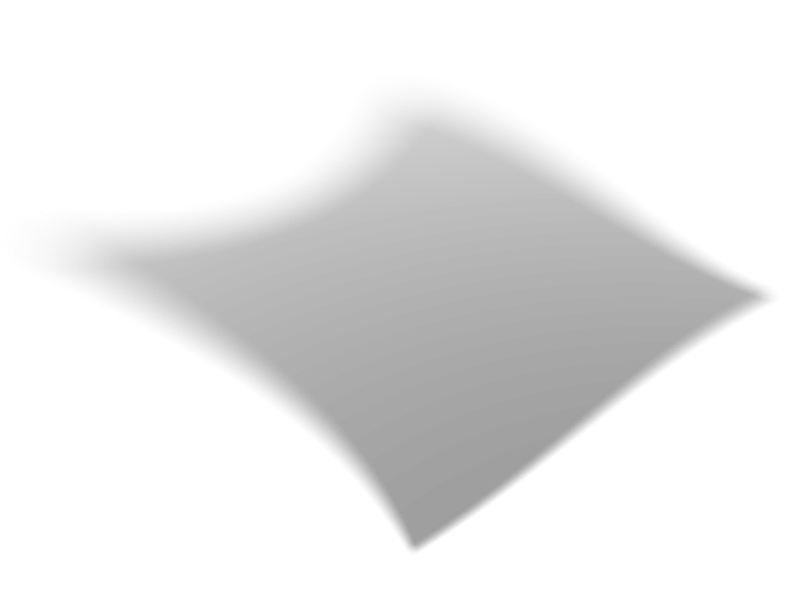
\includegraphics[width=\parampatchimagewidth]{figures/parametric_patch_shadow}};}
% trièdre
\def\scaletriedre{0.85}
\coordinate (o) at (0.20309802889823914 ,  0.26374515891075134);
\coordinate (x) at (0.30103224515914917 ,  0.14841561019420624);
\coordinate (y) at (0.3310101628303528 ,  0.3642595410346985);
\coordinate (z) at (0.17395645380020142 ,  0.43496546149253845);
\draw[axe] (o) -- ($(o)!\scaletriedre!(x)$) node[label, anchor=west] {$x$};
\draw[axe] (o) -- ($(o)!\scaletriedre!(y)$) node[label, anchor=west] {$y$};
\draw[axe] (o) -- ($(o)!\scaletriedre!(z)$) node[label, anchor=south] {$z$};
%
\node[im] at (a) {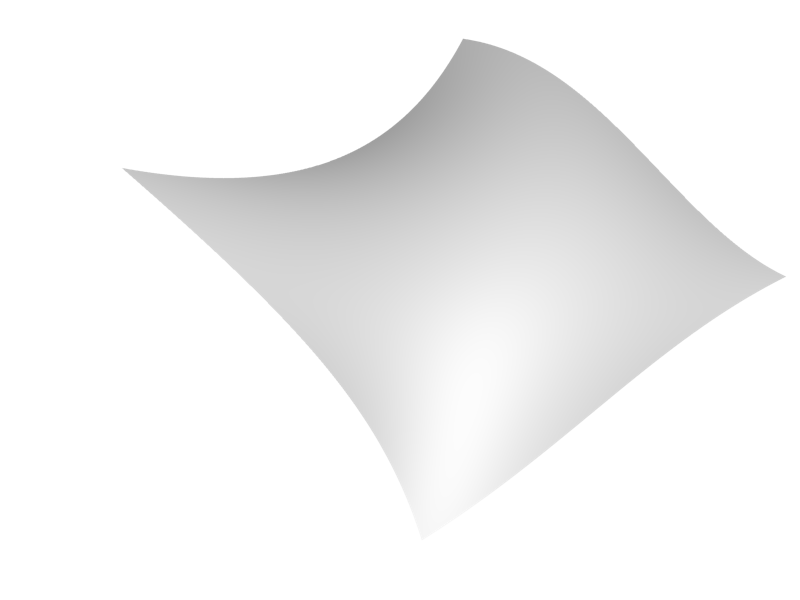
\includegraphics[width=\parampatchimagewidth]{figures/parametric_patch_surface}};
\node[im] at (a) {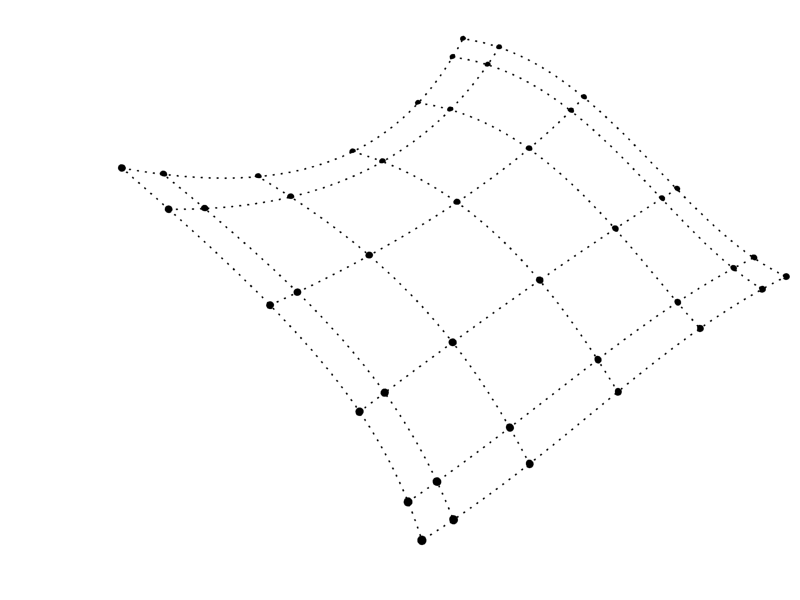
\includegraphics[width=\parampatchimagewidth]{figures/parametric_patch_cgl_grid}};
\node[im] at (a) {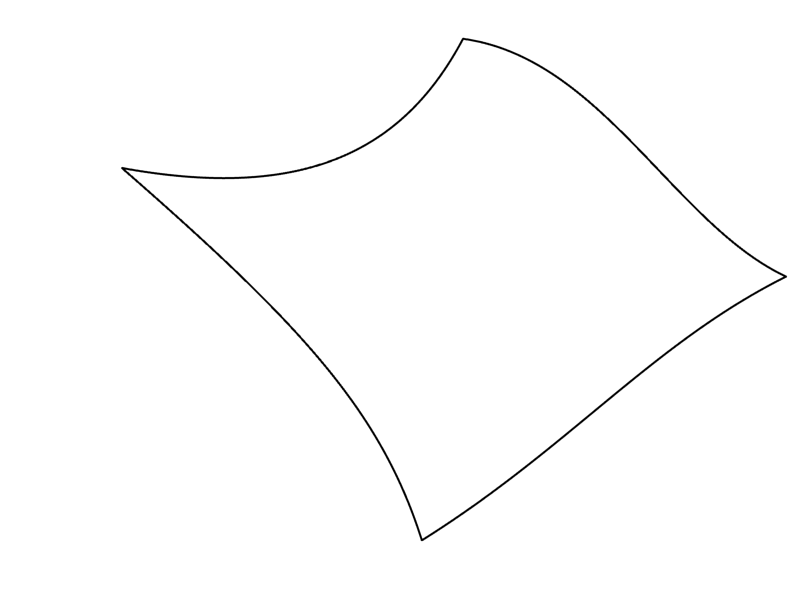
\includegraphics[width=\parampatchimagewidth]{figures/parametric_patch_border}};
% vecteurs
\def\scalevectors{0.99}
\coordinate (s) at (0.5657749772071838, 0.4292657971382141);
\coordinate (u) at (0.6539148092269897, 0.5149791240692139);
\coordinate (v) at (0.506170392036438, 0.5304208993911743);
\coordinate (n) at (0.5878586769104004, 0.5399532318115234);
\draw[vector, red] (s) -- ($(s)!\scalevectors!(u)$) node[label, anchor=north west, xshift=-2pt] {$\bx_u$};
\draw[vector, blue] (s) -- ($(s)!\scalevectors!(v)$) node[label, anchor=east, yshift=-1pt] {$\bx_v$};
\draw[vector, black] (s) -- ($(s)!\scalevectors!(n)$) node[label, anchor=south] {$\unv$};
\node [bigpoint] at (s) {};
\node [label, anchor=north, inner sep=7pt] at (s) {$\bx_{i,j}$};
\end{tikzpicture}%
%\begin{tikzpicture}[
%	im/.style={anchor=north west, inner sep=0pt},
%	bigpoint/.style={circle, fill=black, scale=0.33},
%	axe/.style={-stealth, line width=0.5pt},
%	label/.style={font=\small, inner sep=1.5pt},
%	vector/.style={-latex', very thick}]
%\coordinate (a) at (0,0);
%{\transparent{\parampatchshadowtransparency}\node[im] (shadow) at (a) {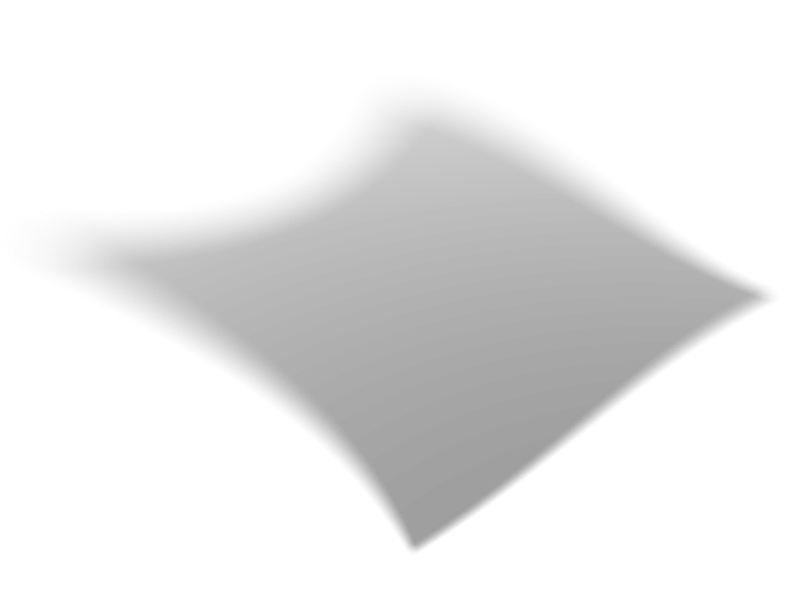
\includegraphics[width=\parampatchimagewidth]{figures/parametric_patch_shadow}};}
%% trièdre
%\def\scaletriedre{0.85}
%\coordinate (o) at ([xshift=14.90mm, yshift=-45.52mm]a);%(16.38mm, -44.12mm);
%\coordinate (x) at ([xshift=22.70mm, yshift=-52.72mm]a);%(26.68mm, -48.84mm);
%\coordinate (y) at ([xshift=25.32mm, yshift=-39.38mm]a);%(24.22mm, -37.05mm);
%\coordinate (z) at ([xshift=12.40mm, yshift=-32.25mm]a);%(13.92mm, -33.98mm);
%\draw[axe] (o) -- ($(o)!\scaletriedre!(x)$) node[label, anchor=west] {$x$};
%\draw[axe] (o) -- ($(o)!\scaletriedre!(y)$) node[label, anchor=west] {$y$};
%\draw[axe] (o) -- ($(o)!\scaletriedre!(z)$) node[label, anchor=south] {$z$};
%%
%\node[im] at (a) {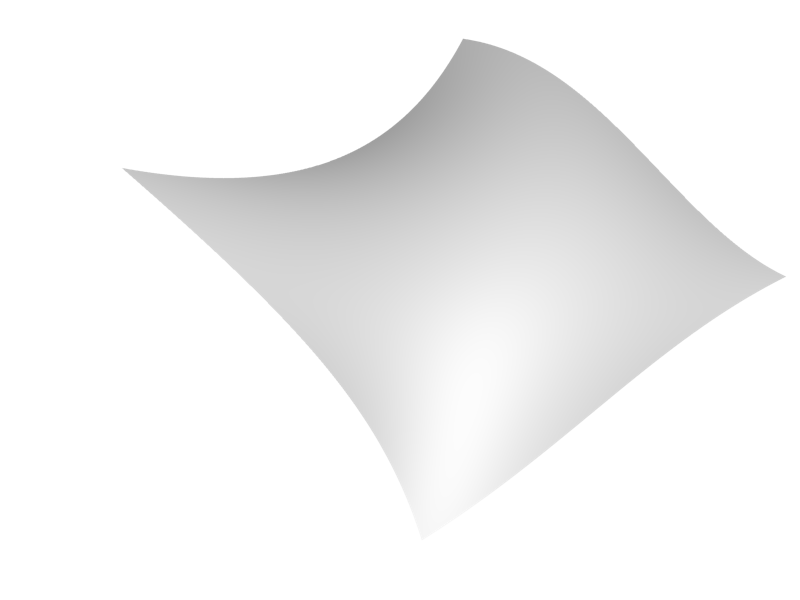
\includegraphics[width=\parampatchimagewidth]{figures/parametric_patch_surface}};
%\node[im] at (a) {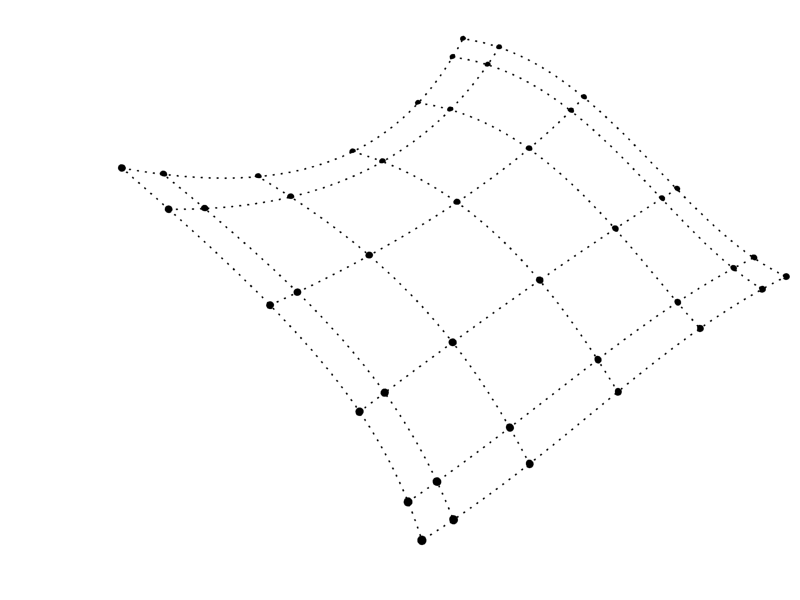
\includegraphics[width=\parampatchimagewidth]{figures/parametric_patch_cgl_grid}};
%\node[im] at (a) {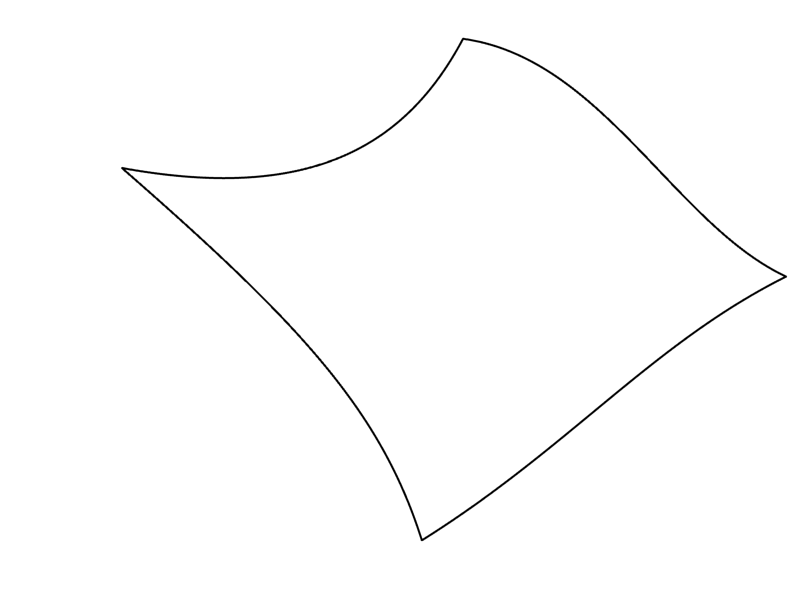
\includegraphics[width=\parampatchimagewidth]{figures/parametric_patch_border}};
%% vecteurs
%\def\scalevectors{0.99}
%\coordinate (s) at ([xshift=45.29mm, yshift=-34.21mm]a);
%\coordinate (u) at ([xshift=52.26mm, yshift=-29.14mm]a);
%\coordinate (v) at ([xshift=40.55mm, yshift=-28.25mm]a);
%\coordinate (n) at ([xshift=47.02mm, yshift=-27.62mm]a);
%\draw[vector, red] (s) -- ($(s)!\scalevectors!(u)$) node[label, anchor=north west, xshift=-2pt] {$\bx_u$};
%\draw[vector, blue] (s) -- ($(s)!\scalevectors!(v)$) node[label, anchor=east, yshift=-1pt] {$\bx_v$};
%\draw[vector, black] (s) -- ($(s)!\scalevectors!(n)$) node[label, anchor=south] {$\unv$};
%\node [bigpoint] at (s) {};
%\node [label, anchor=north, inner sep=7pt] at (s) {$\bx_{i,j}$};
%\end{tikzpicture}%
\label{subfig:cgl_grid_xyz}%
}
\hspace*{\fill}%
\caption{Grille CGL.}%
\label{fig:cgl_grid}%
\end{figure}



\section{Intégration temporelle}%{Discrétisation temporelle}
\begin{itemize}
	\item champ de vitesse connu : intégration classique, schéma explicite (Euler, RK)
	\item vitesse normale connue : approximation EdS
	\begin{itemize}
		\item calcul dérivées par différentiation spectrale
		\item calcul normale et composante tangentielle
%		\item non-linéarités $\to$ aliasing, peut causer instabilité \cite{rahimian2015}
	\end{itemize}
%	\item auto-intersections
%	\begin{itemize}
%		\item globales (traitées au chapitre 3)
%		\item locales \cite{farouki1986}
%	\end{itemize}
\end{itemize}


\section{Instabilités\ldots}
\label{sec:instabilites}
\begin{itemize}
	\item non-linéarités $\to$ aliasing, peut causer instabilité \cite{rahimian2015}, atténuation : sur-échantillonnage, filtrage
	\item auto-intersections
	\begin{itemize}
		\item globales (traitées au \autoref{chap:multi_patch})
		\item locales \cite{farouki1986} (détection, résolution?)
	\end{itemize}
\end{itemize}


\chapter[Généralisation aux surfaces de topologie quelconque]{Généralisation aux surfaces régulières par~morceaux de topologie quelconque}
\label{chap:multi_patch}

\section{Construction des nouvelles faces}

objectif : définir la paramétrisation des nouvelles surfaces (et les limites du domaine paramétrique pour les faces \brep\ reposant sur celles-ci)

\subsection{Arêtes convexes}
paramétrisation approchée des courbes d'intersection (choix du paramètre : abscisse curviligne, paramètre de Hohmeyer (cf. \autoref{sec:calcul_intersections}), \eng{least-square fitting} (ajustement de courbe par la méthode des moindres carrés) d'une série de Chebyshev univariée), portion de \eng{canal surface} approchée 

\subsection{Sommets convexes}
deux variantes :

\subsubsection{Une face polygonale}
$(u,v) \equiv$ coordonnées sphériques\\
+ : 1 seule face, spectre Chebyshev étroit/compact


\subsubsection{Plusieurs faces rectangulaires}
polygone sphérique découpé en quadrilatères \cite{hahn1989}\\
+ : domaine paramétrique non restreint


\section{Résolution des intersections entre faces}
\subsection{État de l'art}
état de l'art méthodes d'intersection de surfaces paramétriques :
review complète \cite{patrikalakis2009}\\
subdivision \cite{houghton1985}, implicitisation approchée \cite{dokken2001}, suivi (marching) \cite{barnhill1990}, Hohmeyer \cite{hohmeyer1992} (critère de détection de boucles sur les enveloppes de normales, paramétrisation monotone et tracé des branches d'intersection)


\subsection{Approche retenue}
\label{sec:calcul_intersections}
adaptation de l'approche de Hohmeyer \cite{hohmeyer1992} (full Chebyshev / Chebyshev-Bernstein)
\begin{itemize}
	\item changement de base \cite{rababah2003}
	\item volumes englobants convexes : oriented bounding box \cite{fournier1994} (détail en \autoref{app:obb}) / enveloppe convexe (comparer complexité, volumes)
	\item subdivision : changement de variable (détail en \autoref{app:cdv_cheb}) / algorithme de Casteljau (ref?) 
	\item test de séparation : théorème de séparation des convexes \cite{eberly2002} / optimisation linéaire \cite{seidel1991}
	\item traitement des intersections tangentielles
\end{itemize}



\section{Validation de la méthode}

\subsection{Propagation suivant un champ de vitesse continu}
sphère/cube dans un écoulement tourbillonnaire incompressible analytique de période temporelle $2T$\\
\begin{equation}
	\vrm{u}(x,y,z,t) = \cos \left( \frac{\pi t}{T} \right)
	\colvec{
	\sin^2(\pi x) \left[ \sin(2\pi z) - \sin(2\pi y)\right] \\
\sin^2(\pi y) \left[ \sin(2\pi x) - \sin(2\pi z)\right] \\
\sin^2(\pi z) \left[ \sin(2\pi y) - \sin(2\pi x)\right]
	}.
\end{equation}
%\begin{figure}
%	\centering
%	\newdimen\imwid
\imwid=0.49\linewidth
\newdimen\rad
\rad=0.12\imwid
\newdimen\ticklen
\ticklen=3pt
\newdimen\imyshift
\imyshift=\rad
\begin{tikzpicture}[%
	img/.style={inner sep=0pt},%
	txt/.style={font=\small, inner sep=2pt},%
	axe/.style={line width=0.5pt}%
	]%
	%
	\node[anchor=south east, yshift=-\imyshift] (im1) {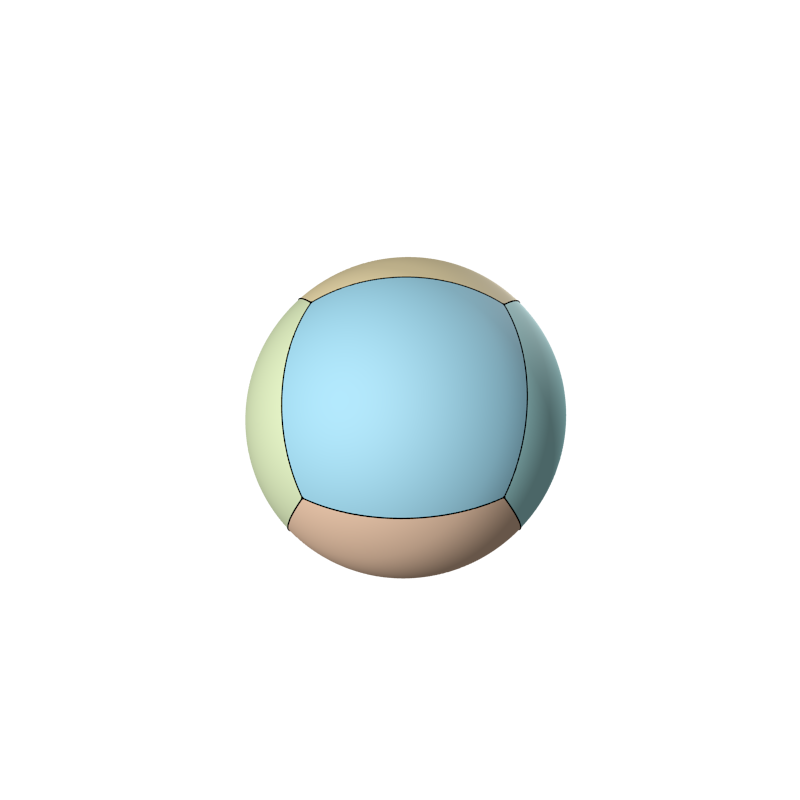
\includegraphics[width=\imwid]{figures/snap_001}};
	\node[anchor=south west, yshift=-\imyshift] (im2) {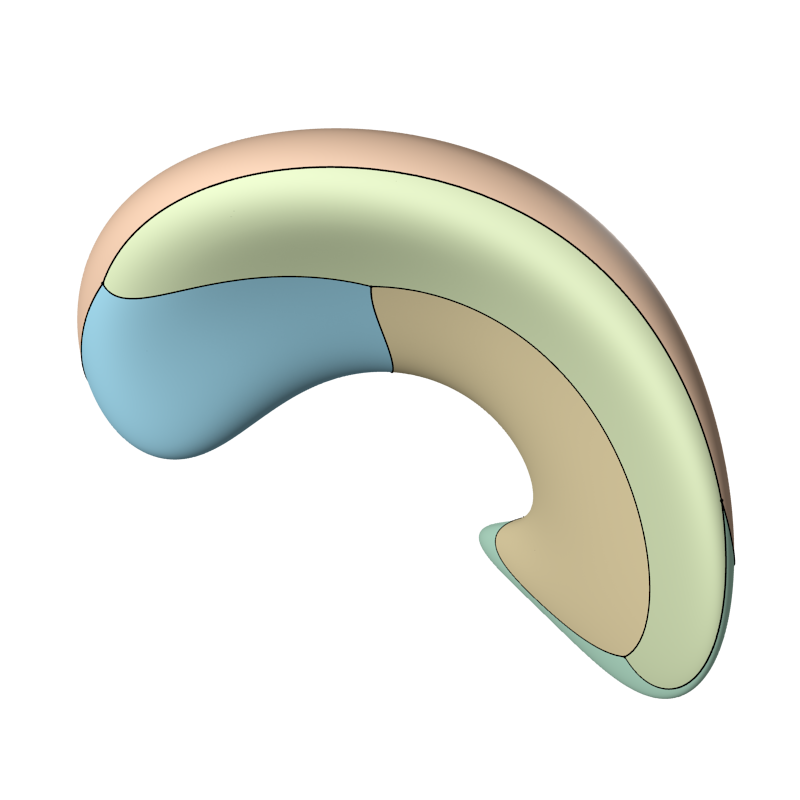
\includegraphics[width=\imwid]{figures/snap_002}};
	\node[anchor=north west, yshift=-\imyshift] (im3) {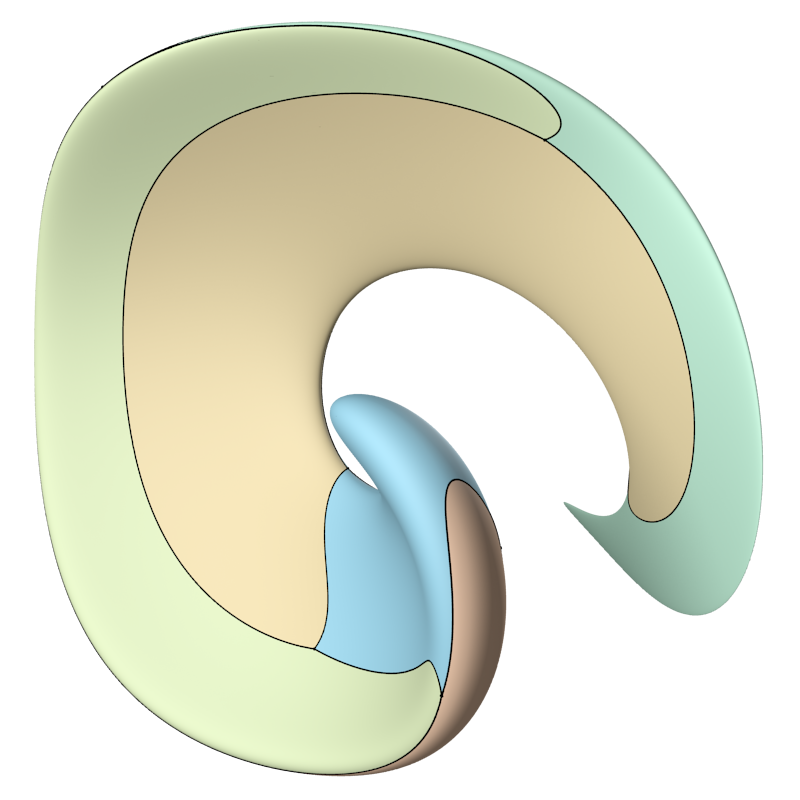
\includegraphics[width=\imwid]{figures/snap_003}};
	\node[anchor=north east, yshift=-\imyshift] (im4) {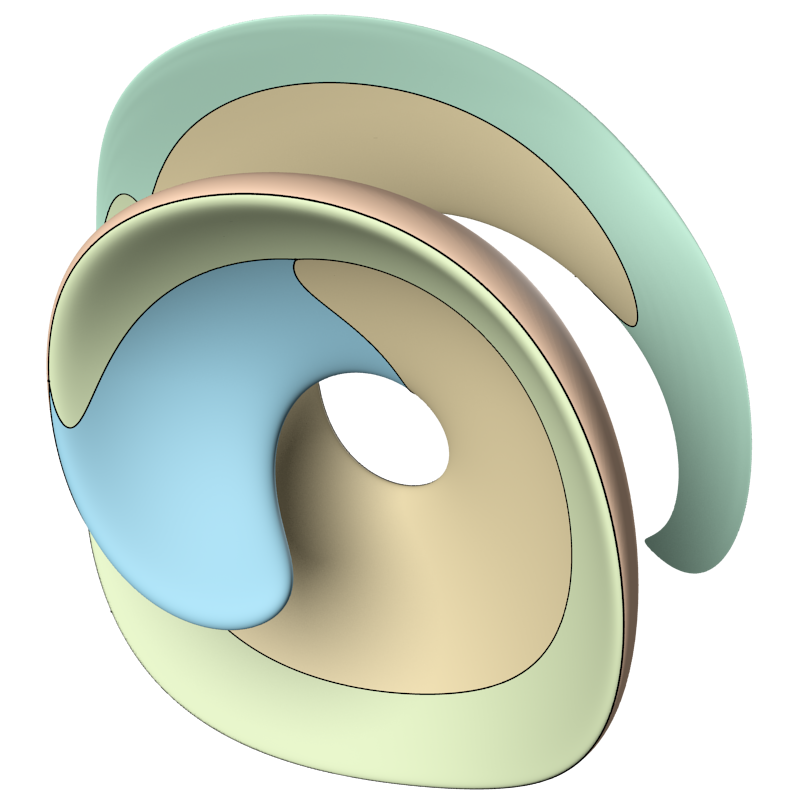
\includegraphics[width=\imwid]{figures/snap_005}};
    %
    \draw[-latex', axe] (0,0) + (135:\rad) arc(135:-180:\rad) node[txt, left, xshift=-1pt] {$t/T$};
    \draw[axe, dash pattern=on 2pt off 2pt] (0,0) + (135:\rad) arc(135:165:\rad);
    \foreach \a in {135,45,-45,-135}
    {%
    	\draw[axe] (\a:\rad-0.5\ticklen)--(\a:\rad+0.5\ticklen);
    }%
    \node[anchor=south east, txt] at (135:\rad) {$0$} ;
    \node[anchor=south west, txt] at (45:\rad) {$1/8$} ;
    \node[anchor=north west, txt] at (-45:\rad) {$1/4$} ;
    \node[anchor=north east, txt] at (-135:\rad) {$1/2$} ;
\end{tikzpicture}
%	\caption{Modèle \brep\ à différents instants de la déformation ($T=4$).}
%	\label{fig:snapshots_vortex}
%\end{figure}

\begin{figure}
	\centering
	\newdimen\imwid
\imwid=0.49\linewidth
\newdimen\imypos
\imypos=1.1\imwid
\def\imangle{0}
\begin{tikzpicture}[%
	img/.style={inner sep=0pt},%
	txt/.style={font=\normalsize, inner sep=2pt, anchor=south west}%
	]%
	%
	\node (im1) at (0,0) {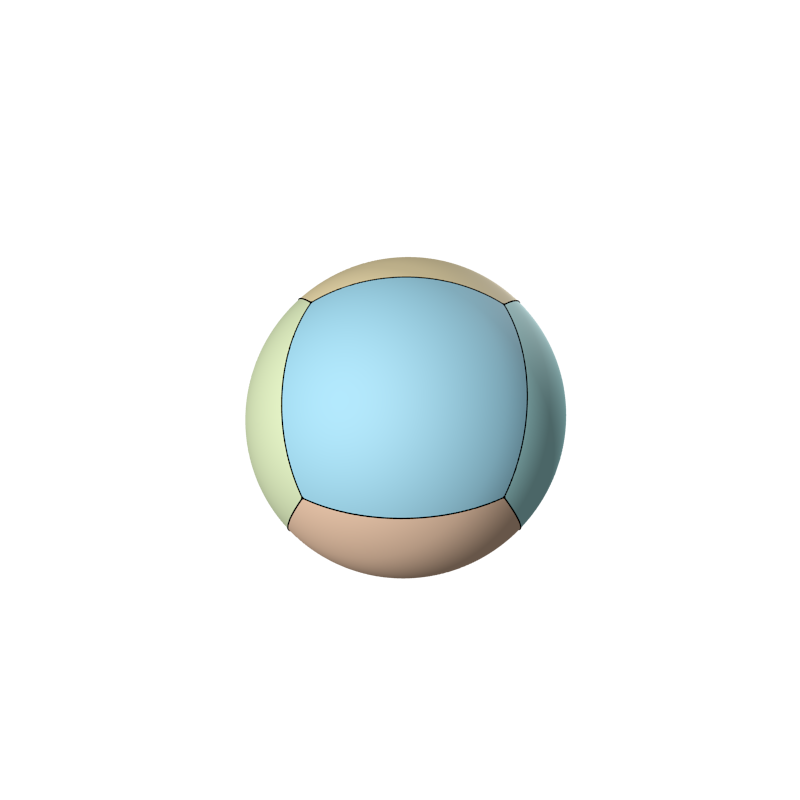
\includegraphics[width=\imwid, angle=\imangle]{figures/snap_001}};
	\node (im2) at (\imwid,0) {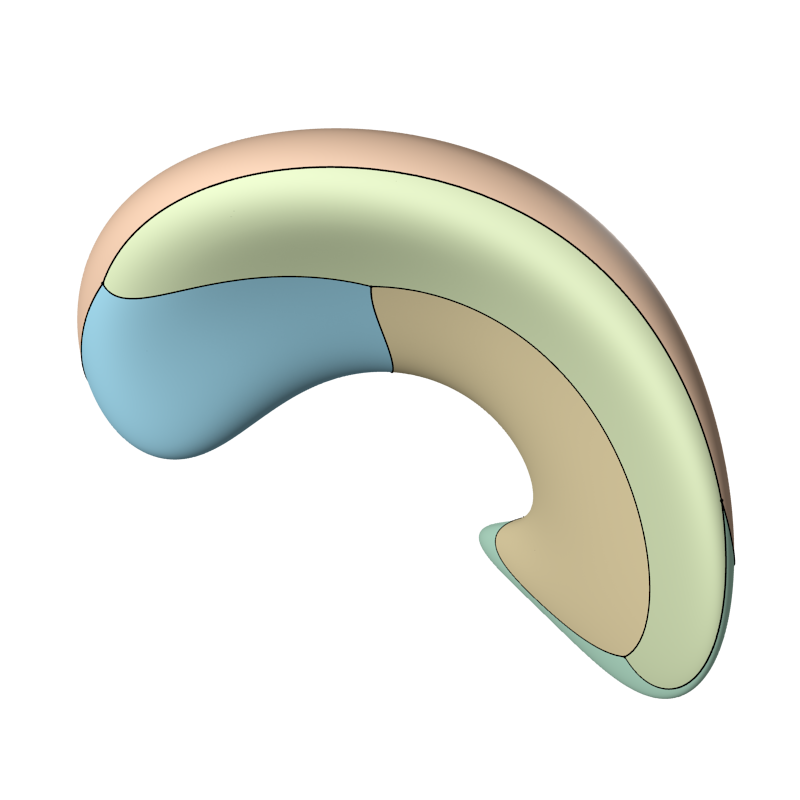
\includegraphics[width=\imwid, angle=\imangle]{figures/snap_002}};
	\node (im3) at (0,-\imypos) {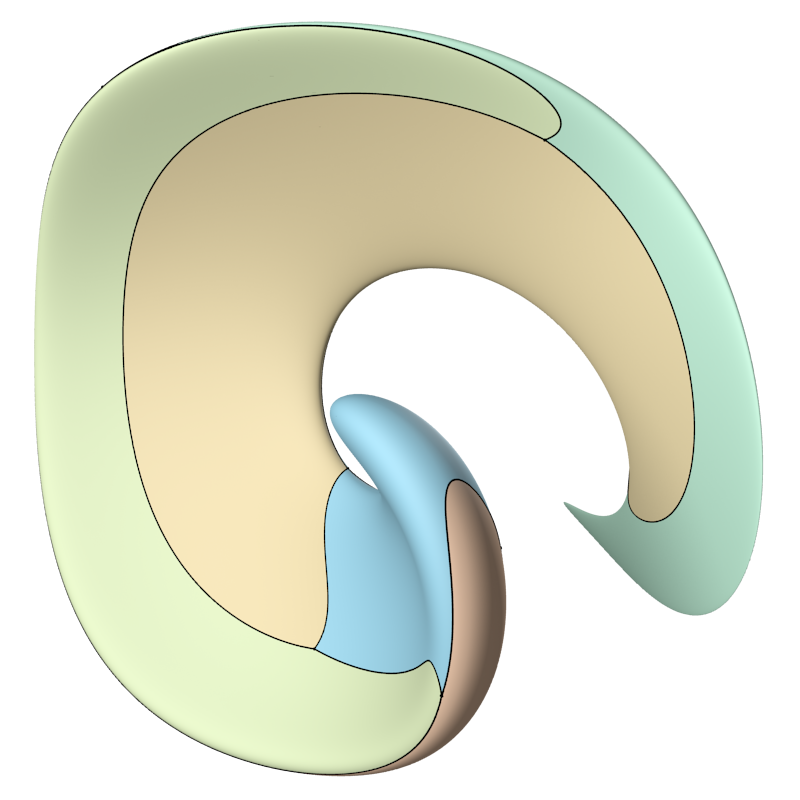
\includegraphics[width=\imwid, angle=\imangle]{figures/snap_003}};
	\node (im4) at (\imwid,-\imypos) {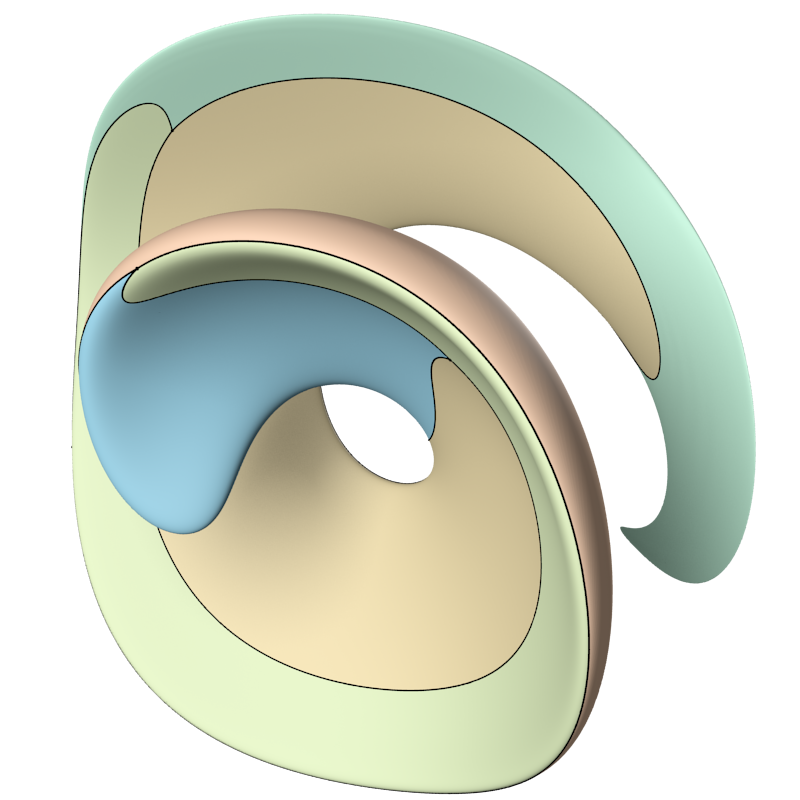
\includegraphics[width=\imwid, angle=\imangle]{figures/snap_004}};
	\node (im5) at (0,-2\imypos) {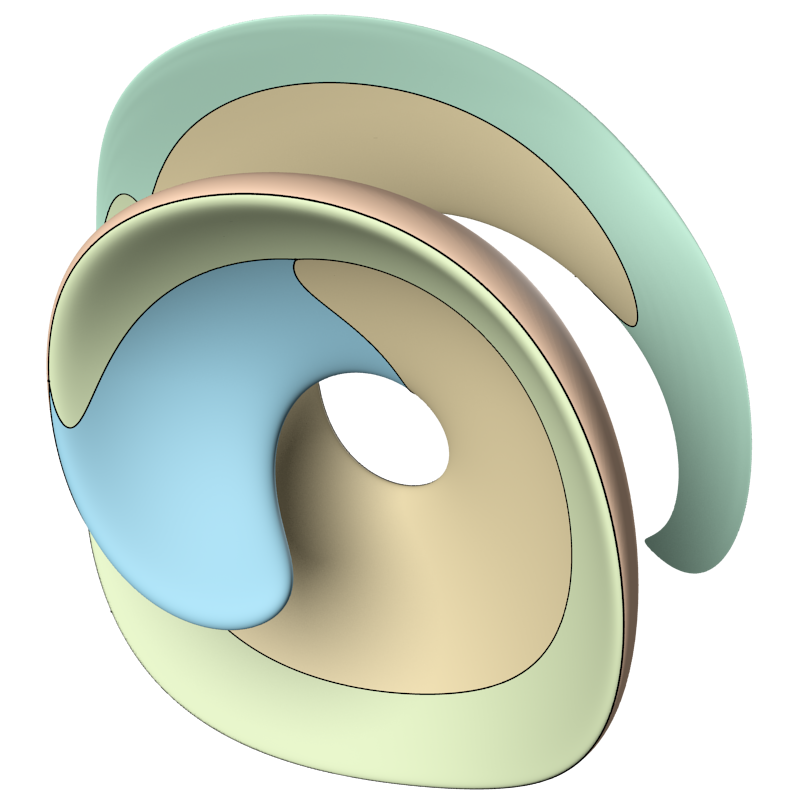
\includegraphics[width=\imwid, angle=\imangle]{figures/snap_005}};
	\node (im6) at (\imwid,-2\imypos) {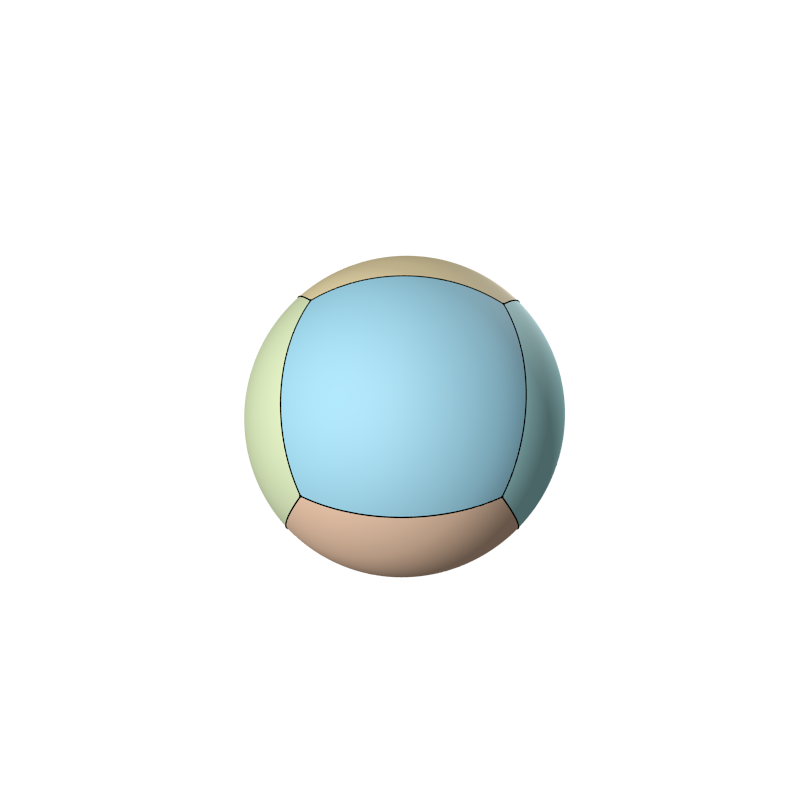
\includegraphics[width=\imwid, angle=\imangle]{figures/snap_006}};
	%
	\node[txt] at (im1.south west) {$t=0$} ;
    \node[txt] at (im2.south west) {$t=T/8$} ;
    \node[txt] at (im3.south west) {$t=T/4$} ;
    \node[txt] at (im4.south west) {$t=3T/8$} ;
    \node[txt] at (im5.south west) {$t=T/2$} ;
    \node[txt] at (im6.south west) {$t=T$} ;
\end{tikzpicture}
	\caption{Modèle \brep\ à différents instants de la déformation ($T=4$).}
	\label{fig:snapshots_vortex}
\end{figure}

calcul de volume avec quadrature de Clenshaw-Curtis (exact, l'intégrande est polynomiale) (étanchéité (continuité $G^0$ partout) garantie car les marqueurs de bord coïncident tout au long de la déformation)\\
convergence de l'erreur d'approximation sur la position, l'aire et le volume à $t = 0$ et $t = T$ pour différents niveaux de discrétisations spatiale et temporelle\\

%%%%%%%%%%%%%%%
% figures erreur vs dof
%%%%%%%%%%%%%%
\def\axw{0.48\textwidth}
\def\axh{0.39\textwidth}
\def\xlabl{dof}
\def\ylabl{Erreur}
\def\xsep{2pt}
%%%%%%%%%%%%%%
\plotvortexerror{position}{la~}{pos}{maximale}
%%%%%%%%%%%%%%
\plotvortexerror{aire}{l'}{air}{relative}
%%%%%%%%%%%%%%
\plotvortexerror{volume}{le~}{vol}{relative}
%%%%%%%%%%%%%%
%%%%%%%%%%%%%%


+ convergence de la variation de volume au cours de la déformation\\
\tabularnums{\liningnums{1234567890}}\\
\proportionalnums{\liningnums{1234567890}}\\
\tabularnums{\oldstylenums{1234567890}}\\
\proportionalnums{\oldstylenums{1234567890}}
%https://tex.stackexchange.com/questions/23993/use-first-row-of-a-table-as-legend-entry-in-pgfplot-graph
\begin{figure}
  \centering
  \begin{tikzpicture}%
  \begin{semilogyaxis}[%
    axis lines*=left,%
    width=9cm, height=7cm,%
    xmin = 0.0, xmax = 1.0,%
    %ymin = 1e-16, ymax = 1e1,%
    %ytickten = {-15,-10,-5,0},%
    ymin = 1e-15, ymax = 1e0,%
    ytickten = {-15,-10,-5,0},%
    grid=major,%
    xlabel={$t/T$},%
    ylabel={$\frac{\left|V - V_0\right|}{V_0}$},%
    %legend style={font=\small, at={(0.5,0.0)}, anchor=south, yshift=4pt},%
    legend style={font=\small, at={(1.025,1.0)}, anchor=north west},%
    no marks, each nth point=1]%
    \pgfplotstableread{figures/data/vortex_erreur_volume_vs_time_0.001.dat}   {\datatable}
    \pgfplotstablegetcolsof{\datatable}
    \pgfmathtruncatemacro\numberofcols{\pgfplotsretval-1}
    \pgfplotsinvokeforeach{2,...,\numberofcols}{
      \pgfplotstablegetcolumnnamebyindex{#1}\of{\datatable}\to{\colname}
      \addplot+ table [y index=#1] from \datatable;%
  	  \addlegendentryexpanded{$\mathrm{dof} = \colname$}
    }%
  \end{semilogyaxis}%
  \end{tikzpicture}%
  \caption{Évolution de l'erreur relative en volume au cours du temps, pour différents niveaux de discrétisation spatiale. Le schéma de Runge-Kutta explicite à l'ordre 4 est utilisé pour l'intégration temporelle, avec un pas de temps $\Delta t = 0.001$.}
\end{figure}

\subsection{Propagation à vitesse normale uniforme}
cube en expansion
\begin{figure}
	\centering
	%\textit{snapshots surface déformée}
	\newdimen\imwid
	\imwid=0.32\linewidth
	\begin{tikzpicture}
		\foreach [count=\i] \l in {{0}, {1}, {2}}
		{%
			\node (im\i) at (\i\imwid,0) {\includegraphics[width=\imwid]{figures/cube_brep_t\i}};
			\node[inner sep=0pt] (lab\i) at (im\i.south) {$t = \l$};
		}%
	\end{tikzpicture}
	\caption{\ldots}
	\label{fig:snapshots_cube}
\end{figure}

\subsection{Propagation à vitesse normale non uniforme?}
?


\chapter{Déformation de maillage surfacique}

\chapter{Application à la simulation de la régression de propergol solide}

\def\chapterabstract{}
\chapter*{Conclusion}
\chaptermark{Conclusion}
\addcontentsline{toc}{chapter}{Conclusion}



% APPENDICES
\appendix
%\chapter{Une annexe}
%\label{annex:test}
%\lipsum[1-5]


\backmatter
\cleardoublepage
\phantomsection

% BIBLIOGRAPHIE
\nocite{*}
%\pagestyle{mypagestylebiblio} % workaround for correct headings
\bibliographystyle{mybibstyle}
%\bibliography{biblio}
\bibliography{biblio/intersections,biblio/chebyshev,biblio/interface_propagation,biblio/spectral,biblio/moving_geometries,biblio/mesh.bib}

\end{document}